% Options for packages loaded elsewhere
\PassOptionsToPackage{unicode}{hyperref}
\PassOptionsToPackage{hyphens}{url}
\documentclass[
]{article}
\usepackage{xcolor}
\usepackage[margin=1in]{geometry}
\usepackage{amsmath,amssymb}
\setcounter{secnumdepth}{5}
\usepackage{iftex}
\ifPDFTeX
  \usepackage[T1]{fontenc}
  \usepackage[utf8]{inputenc}
  \usepackage{textcomp} % provide euro and other symbols
\else % if luatex or xetex
  \usepackage{unicode-math} % this also loads fontspec
  \defaultfontfeatures{Scale=MatchLowercase}
  \defaultfontfeatures[\rmfamily]{Ligatures=TeX,Scale=1}
\fi
\usepackage{lmodern}
\ifPDFTeX\else
  % xetex/luatex font selection
\fi
% Use upquote if available, for straight quotes in verbatim environments
\IfFileExists{upquote.sty}{\usepackage{upquote}}{}
\IfFileExists{microtype.sty}{% use microtype if available
  \usepackage[]{microtype}
  \UseMicrotypeSet[protrusion]{basicmath} % disable protrusion for tt fonts
}{}
\makeatletter
\@ifundefined{KOMAClassName}{% if non-KOMA class
  \IfFileExists{parskip.sty}{%
    \usepackage{parskip}
  }{% else
    \setlength{\parindent}{0pt}
    \setlength{\parskip}{6pt plus 2pt minus 1pt}}
}{% if KOMA class
  \KOMAoptions{parskip=half}}
\makeatother
\usepackage{color}
\usepackage{fancyvrb}
\newcommand{\VerbBar}{|}
\newcommand{\VERB}{\Verb[commandchars=\\\{\}]}
\DefineVerbatimEnvironment{Highlighting}{Verbatim}{commandchars=\\\{\}}
% Add ',fontsize=\small' for more characters per line
\usepackage{framed}
\definecolor{shadecolor}{RGB}{248,248,248}
\newenvironment{Shaded}{\begin{snugshade}}{\end{snugshade}}
\newcommand{\AlertTok}[1]{\textcolor[rgb]{0.94,0.16,0.16}{#1}}
\newcommand{\AnnotationTok}[1]{\textcolor[rgb]{0.56,0.35,0.01}{\textbf{\textit{#1}}}}
\newcommand{\AttributeTok}[1]{\textcolor[rgb]{0.13,0.29,0.53}{#1}}
\newcommand{\BaseNTok}[1]{\textcolor[rgb]{0.00,0.00,0.81}{#1}}
\newcommand{\BuiltInTok}[1]{#1}
\newcommand{\CharTok}[1]{\textcolor[rgb]{0.31,0.60,0.02}{#1}}
\newcommand{\CommentTok}[1]{\textcolor[rgb]{0.56,0.35,0.01}{\textit{#1}}}
\newcommand{\CommentVarTok}[1]{\textcolor[rgb]{0.56,0.35,0.01}{\textbf{\textit{#1}}}}
\newcommand{\ConstantTok}[1]{\textcolor[rgb]{0.56,0.35,0.01}{#1}}
\newcommand{\ControlFlowTok}[1]{\textcolor[rgb]{0.13,0.29,0.53}{\textbf{#1}}}
\newcommand{\DataTypeTok}[1]{\textcolor[rgb]{0.13,0.29,0.53}{#1}}
\newcommand{\DecValTok}[1]{\textcolor[rgb]{0.00,0.00,0.81}{#1}}
\newcommand{\DocumentationTok}[1]{\textcolor[rgb]{0.56,0.35,0.01}{\textbf{\textit{#1}}}}
\newcommand{\ErrorTok}[1]{\textcolor[rgb]{0.64,0.00,0.00}{\textbf{#1}}}
\newcommand{\ExtensionTok}[1]{#1}
\newcommand{\FloatTok}[1]{\textcolor[rgb]{0.00,0.00,0.81}{#1}}
\newcommand{\FunctionTok}[1]{\textcolor[rgb]{0.13,0.29,0.53}{\textbf{#1}}}
\newcommand{\ImportTok}[1]{#1}
\newcommand{\InformationTok}[1]{\textcolor[rgb]{0.56,0.35,0.01}{\textbf{\textit{#1}}}}
\newcommand{\KeywordTok}[1]{\textcolor[rgb]{0.13,0.29,0.53}{\textbf{#1}}}
\newcommand{\NormalTok}[1]{#1}
\newcommand{\OperatorTok}[1]{\textcolor[rgb]{0.81,0.36,0.00}{\textbf{#1}}}
\newcommand{\OtherTok}[1]{\textcolor[rgb]{0.56,0.35,0.01}{#1}}
\newcommand{\PreprocessorTok}[1]{\textcolor[rgb]{0.56,0.35,0.01}{\textit{#1}}}
\newcommand{\RegionMarkerTok}[1]{#1}
\newcommand{\SpecialCharTok}[1]{\textcolor[rgb]{0.81,0.36,0.00}{\textbf{#1}}}
\newcommand{\SpecialStringTok}[1]{\textcolor[rgb]{0.31,0.60,0.02}{#1}}
\newcommand{\StringTok}[1]{\textcolor[rgb]{0.31,0.60,0.02}{#1}}
\newcommand{\VariableTok}[1]{\textcolor[rgb]{0.00,0.00,0.00}{#1}}
\newcommand{\VerbatimStringTok}[1]{\textcolor[rgb]{0.31,0.60,0.02}{#1}}
\newcommand{\WarningTok}[1]{\textcolor[rgb]{0.56,0.35,0.01}{\textbf{\textit{#1}}}}
\usepackage{graphicx}
\makeatletter
\newsavebox\pandoc@box
\newcommand*\pandocbounded[1]{% scales image to fit in text height/width
  \sbox\pandoc@box{#1}%
  \Gscale@div\@tempa{\textheight}{\dimexpr\ht\pandoc@box+\dp\pandoc@box\relax}%
  \Gscale@div\@tempb{\linewidth}{\wd\pandoc@box}%
  \ifdim\@tempb\p@<\@tempa\p@\let\@tempa\@tempb\fi% select the smaller of both
  \ifdim\@tempa\p@<\p@\scalebox{\@tempa}{\usebox\pandoc@box}%
  \else\usebox{\pandoc@box}%
  \fi%
}
% Set default figure placement to htbp
\def\fps@figure{htbp}
\makeatother
\setlength{\emergencystretch}{3em} % prevent overfull lines
\providecommand{\tightlist}{%
  \setlength{\itemsep}{0pt}\setlength{\parskip}{0pt}}
\usepackage{booktabs}
\usepackage{longtable}
\usepackage{array}
\usepackage{multirow}
\usepackage{wrapfig}
\usepackage{float}
\usepackage{colortbl}
\usepackage{pdflscape}
\usepackage{tabu}
\usepackage{threeparttable}
\usepackage{threeparttablex}
\usepackage[normalem]{ulem}
\usepackage{makecell}
\usepackage{xcolor}
\usepackage{bookmark}
\IfFileExists{xurl.sty}{\usepackage{xurl}}{} % add URL line breaks if available
\urlstyle{same}
\hypersetup{
  pdftitle={Technical Report},
  pdfauthor={{[}Author Name{]}},
  hidelinks,
  pdfcreator={LaTeX via pandoc}}

\title{Technical Report}
\author{{[}Author Name{]}}
\date{2026-04-23}

\begin{document}
\maketitle

{
\setcounter{tocdepth}{3}
\tableofcontents
}
\section{Setup and Imports}\label{setup-and-imports}

This technical report documents the implementation and results of nine
Weibull parameter estimation methods applied to Backblaze hard drive
failure data. All code is shown (\texttt{echo\ =\ TRUE}).

\begin{Shaded}
\begin{Highlighting}[]
\NormalTok{drives  }\OtherTok{\textless{}{-}} \FunctionTok{read\_csv}\NormalTok{(}\StringTok{"../data/drives\_clean.csv"}\NormalTok{, }\AttributeTok{show\_col\_types =} \ConstantTok{FALSE}\NormalTok{)}
\NormalTok{params  }\OtherTok{\textless{}{-}} \FunctionTok{read\_csv}\NormalTok{(}\StringTok{"results/parameters.csv"}\NormalTok{, }\AttributeTok{show\_col\_types =} \ConstantTok{FALSE}\NormalTok{)}
\NormalTok{gof     }\OtherTok{\textless{}{-}} \FunctionTok{read\_csv}\NormalTok{(}\StringTok{"results/gof\_metrics.csv"}\NormalTok{, }\AttributeTok{show\_col\_types =} \ConstantTok{FALSE}\NormalTok{)}
\NormalTok{summary }\OtherTok{\textless{}{-}} \FunctionTok{read\_csv}\NormalTok{(}\StringTok{"../data/model\_summary.csv"}\NormalTok{, }\AttributeTok{show\_col\_types =} \ConstantTok{FALSE}\NormalTok{)}
\NormalTok{models  }\OtherTok{\textless{}{-}} \FunctionTok{unique}\NormalTok{(drives}\SpecialCharTok{$}\NormalTok{model)}
\end{Highlighting}
\end{Shaded}

\section{Data Loading and
Preprocessing}\label{data-loading-and-preprocessing}

The Backblaze Q3 2025 dataset was processed according to the pipeline in
\texttt{01\_data\_prep.R}. Each daily CSV contains one row per drive. We
collapse to one row per drive with \texttt{lifetime\_days},
\texttt{failed}, and \texttt{model}.

\begin{Shaded}
\begin{Highlighting}[]
\NormalTok{summary }\SpecialCharTok{\%\textgreater{}\%}
  \FunctionTok{kable}\NormalTok{(}\AttributeTok{caption =} \StringTok{"Per{-}Model Drive Summary"}\NormalTok{,}
        \AttributeTok{col.names =} \FunctionTok{c}\NormalTok{(}\StringTok{"Model"}\NormalTok{, }\StringTok{"N Total"}\NormalTok{, }\StringTok{"Failures"}\NormalTok{, }\StringTok{"Censored"}\NormalTok{,}
                      \StringTok{"Censoring \%"}\NormalTok{, }\StringTok{"Min Days"}\NormalTok{, }\StringTok{"Median Days"}\NormalTok{, }\StringTok{"Max Days"}\NormalTok{),}
        \AttributeTok{booktabs =} \ConstantTok{TRUE}\NormalTok{) }\SpecialCharTok{\%\textgreater{}\%}
  \FunctionTok{kable\_styling}\NormalTok{(}\AttributeTok{latex\_options =} \FunctionTok{c}\NormalTok{(}\StringTok{"striped"}\NormalTok{, }\StringTok{"hold\_position"}\NormalTok{))}
\end{Highlighting}
\end{Shaded}

\begin{longtable}[t]{lrrrrrrr}
\caption{\label{tab:data-summary}Per-Model Drive Summary}\\
\toprule
Model & N Total & Failures & Censored & Censoring \% & Min Days & Median Days & Max Days\\
\midrule
\cellcolor{gray!10}{TOSHIBA MG07ACA14TA} & \cellcolor{gray!10}{37463} & \cellcolor{gray!10}{116} & \cellcolor{gray!10}{37347} & \cellcolor{gray!10}{99.69} & \cellcolor{gray!10}{1} & \cellcolor{gray!10}{92} & \cellcolor{gray!10}{92}\\
TOSHIBA MG08ACA16TA & 40184 & 85 & 40099 & 99.79 & 1 & 92 & 92\\
\cellcolor{gray!10}{WDC WUH722222ALE6L4} & \cellcolor{gray!10}{40271} & \cellcolor{gray!10}{50} & \cellcolor{gray!10}{40221} & \cellcolor{gray!10}{99.88} & \cellcolor{gray!10}{1} & \cellcolor{gray!10}{92} & \cellcolor{gray!10}{92}\\
\bottomrule
\end{longtable}

\textbf{Right-censoring}: drives with \texttt{failed\ =\ 0} survived at
least \texttt{lifetime\_days} but their true failure time is unknown.
Ignoring censored units systematically biases all estimates.

\section{Estimation Methods}\label{estimation-methods}

\subsection{2.1 OLS (Ordinary Least Squares /
MRR)}\label{ols-ordinary-least-squares-mrr}

The Weibull CDF is linearized:
\[\ln(-\ln(1 - F(t))) = k \cdot \ln(t) - k \cdot \ln(\lambda)\]

Median ranks via Benard's formula:
\[\hat{F}_i = \frac{i - 0.3}{n + 0.4}\]

OLS regression: \(Y = k \cdot X + b\) where
\(Y_i = \ln(-\ln(1-\hat{F}_i))\), \(X_i = \ln(t_i)\).

\begin{Shaded}
\begin{Highlighting}[]
\CommentTok{\# Example: first model}
\NormalTok{mdl }\OtherTok{\textless{}{-}}\NormalTok{ models[}\DecValTok{1}\NormalTok{]}
\NormalTok{t\_fail }\OtherTok{\textless{}{-}} \FunctionTok{sort}\NormalTok{(drives}\SpecialCharTok{$}\NormalTok{lifetime\_days[drives}\SpecialCharTok{$}\NormalTok{model }\SpecialCharTok{==}\NormalTok{ mdl }\SpecialCharTok{\&}\NormalTok{ drives}\SpecialCharTok{$}\NormalTok{failed }\SpecialCharTok{==} \DecValTok{1}\NormalTok{])}
\NormalTok{n }\OtherTok{\textless{}{-}} \FunctionTok{length}\NormalTok{(t\_fail)}
\NormalTok{F\_i }\OtherTok{\textless{}{-}}\NormalTok{ ((}\DecValTok{1}\SpecialCharTok{:}\NormalTok{n) }\SpecialCharTok{{-}} \FloatTok{0.3}\NormalTok{) }\SpecialCharTok{/}\NormalTok{ (n }\SpecialCharTok{+} \FloatTok{0.4}\NormalTok{)}
\NormalTok{Y }\OtherTok{\textless{}{-}} \FunctionTok{log}\NormalTok{(}\SpecialCharTok{{-}}\FunctionTok{log}\NormalTok{(}\DecValTok{1} \SpecialCharTok{{-}}\NormalTok{ F\_i))}
\NormalTok{X }\OtherTok{\textless{}{-}} \FunctionTok{log}\NormalTok{(t\_fail)}
\NormalTok{fit }\OtherTok{\textless{}{-}} \FunctionTok{lm}\NormalTok{(Y }\SpecialCharTok{\textasciitilde{}}\NormalTok{ X)}
\FunctionTok{cat}\NormalTok{(}\StringTok{"OLS for"}\NormalTok{, mdl, }\StringTok{": k ="}\NormalTok{, }\FunctionTok{coef}\NormalTok{(fit)[}\DecValTok{2}\NormalTok{], }\StringTok{", lambda ="}\NormalTok{, }\FunctionTok{exp}\NormalTok{(}\SpecialCharTok{{-}}\FunctionTok{coef}\NormalTok{(fit)[}\DecValTok{1}\NormalTok{]}\SpecialCharTok{/}\FunctionTok{coef}\NormalTok{(fit)[}\DecValTok{2}\NormalTok{]))}
\end{Highlighting}
\end{Shaded}

\begin{verbatim}
## OLS for TOSHIBA MG07ACA14TA : k = 1.23859 , lambda = 53.8531
\end{verbatim}

\textbf{Note}: OLS = MRR in reliability engineering literature.
Identical computation.

\subsection{2.2 WLS (Weighted Least Squares --- Bergman
Weights)}\label{wls-weighted-least-squares-bergman-weights}

Bergman (1986) weights via delta method:
\[w_i = \frac{[(1-F_i)(-\ln(1-F_i))]^2 \cdot (N+1)^2(N+2)}{i(N-i+1)}\]

Weight peaks at \(F \approx 0.632\) (the Weibull characteristic life
point). WLS can outrank MLE when the true distribution is only
approximately Weibull.

\subsection{2.3 MOM (Method of Moments)}\label{mom-method-of-moments}

\[CV^2 = \frac{\Gamma(1+2/k)}{\Gamma(1+1/k)^2} - 1\]

\textbf{Universal pattern}: \(\lambda\) cancels in any dimensionless
moment ratio. CV², \(\tau_2\), EPF all depend only on \(k\).

Biased under \textbf{any} censoring fraction \textgreater{} 0\%.

\subsection{2.4 L-Moments}\label{l-moments}

Closed-form solution:
\[k = \frac{-\ln 2}{\ln(1 - \tau_2)}, \quad \tau_2 = \frac{\lambda_2}{L_1}\]

More robust than MOM: linear combinations amplify outliers linearly, not
quadratically.

\subsection{2.5 EPF (Energy Pattern
Factor)}\label{epf-energy-pattern-factor}

\[EPF = \frac{\Gamma(1+3/k)}{\Gamma(1+1/k)^3} \quad [\lambda^3 \text{ cancels}]\]

Root-finding bracket: \([0.5, 20]\). Empirical approximation
\(k \approx 1 + 3.69/EPF^2\) valid only for \(k \in [1,3]\).

\subsection{2.6 MLE (Maximum Likelihood)}\label{mle-maximum-likelihood}

Censored log-likelihood:
\[\ell(k,\lambda) = \sum_{\text{fail}} \left[\ln k - \ln\lambda + (k-1)\ln\frac{t}{\lambda} - \left(\frac{t}{\lambda}\right)^k\right] + \sum_{\text{cens}} \left[-\left(\frac{t}{\lambda}\right)^k\right]\]

Optimized via Nelder-Mead on log scale.

\subsection{2.7A MAP (Bayesian Maximum A
Posteriori)}\label{a-map-bayesian-maximum-a-posteriori}

Same likelihood + exponential priors:
\[\pi(k) \propto e^{-k/\mu_k}, \quad \pi(\lambda) \propto e^{-\lambda/\bar{t}_f}\]

\textbf{Critical}: flat prior + MAP = MLE exactly (\(\ln 1 = 0\)).
Exponential prior adds regularization.

\subsection{2.7B MCMC (Full Bayesian ---
Extension)}\label{b-mcmc-full-bayesian-extension}

\textbf{This method is an EXTENSION beyond core course materials.}

Full posterior via brms/Stan (HMC-NUTS). Returns credible intervals. MAP
gives false precision; MCMC gives honest uncertainty.

\subsection{2.8 Percentile}\label{percentile}

Two points \(p_1 = 0.16\), \(p_2 = 0.84\):
\[k = \frac{\ln(-\ln(1-p_2)) - \ln(-\ln(1-p_1))}{\ln t_2 - \ln t_1}\]

Uses only 2 of \(n\) points. Pedagogical baseline.

\section{GoF Metrics}\label{gof-metrics}

\begin{Shaded}
\begin{Highlighting}[]
\NormalTok{gof }\SpecialCharTok{\%\textgreater{}\%}
  \FunctionTok{select}\NormalTok{(model, method, KS, RMSE, MAE, AD, AIC, BIC, MRL\_err, Composite\_Rank) }\SpecialCharTok{\%\textgreater{}\%}
  \FunctionTok{mutate}\NormalTok{(}\FunctionTok{across}\NormalTok{(}\FunctionTok{where}\NormalTok{(is.numeric), }\SpecialCharTok{\textasciitilde{}}\FunctionTok{round}\NormalTok{(., }\DecValTok{4}\NormalTok{))) }\SpecialCharTok{\%\textgreater{}\%}
  \FunctionTok{kable}\NormalTok{(}\AttributeTok{caption =} \StringTok{"Goodness{-}of{-}Fit Metrics — All Models"}\NormalTok{,}
        \AttributeTok{booktabs =} \ConstantTok{TRUE}\NormalTok{, }\AttributeTok{longtable =} \ConstantTok{TRUE}\NormalTok{) }\SpecialCharTok{\%\textgreater{}\%}
  \FunctionTok{kable\_styling}\NormalTok{(}\AttributeTok{latex\_options =} \FunctionTok{c}\NormalTok{(}\StringTok{"striped"}\NormalTok{, }\StringTok{"hold\_position"}\NormalTok{, }\StringTok{"repeat\_header"}\NormalTok{),}
                \AttributeTok{font\_size =} \DecValTok{8}\NormalTok{)}
\end{Highlighting}
\end{Shaded}

\begingroup\fontsize{8}{10}\selectfont

\begin{longtable}[t]{llrrrrrrrr}
\caption{\label{tab:gof-table}Goodness-of-Fit Metrics — All Models}\\
\toprule
model & method & KS & RMSE & MAE & AD & AIC & BIC & MRL\_err & Composite\_Rank\\
\midrule
\endfirsthead
\caption[]{Goodness-of-Fit Metrics — All Models \textit{(continued)}}\\
\toprule
model & method & KS & RMSE & MAE & AD & AIC & BIC & MRL\_err & Composite\_Rank\\
\midrule
\endhead

\endfoot
\bottomrule
\endlastfoot
\cellcolor{gray!10}{TOSHIBA MG07ACA14TA} & \cellcolor{gray!10}{OLS} & \cellcolor{gray!10}{0.1375} & \cellcolor{gray!10}{0.0586} & \cellcolor{gray!10}{0.0483} & \cellcolor{gray!10}{3.0372} & \cellcolor{gray!10}{146091.89} & \cellcolor{gray!10}{146108.96} & \cellcolor{gray!10}{9.8674} & \cellcolor{gray!10}{4.6667}\\
TOSHIBA MG07ACA14TA & WLS & 0.1145 & 0.0448 & 0.0333 & 1.9922 & 169173.38 & 169190.44 & 5.0273 & 2.6667\\
\cellcolor{gray!10}{TOSHIBA MG07ACA14TA} & \cellcolor{gray!10}{MOM} & \cellcolor{gray!10}{0.1438} & \cellcolor{gray!10}{0.0559} & \cellcolor{gray!10}{0.0455} & \cellcolor{gray!10}{2.7008} & \cellcolor{gray!10}{213664.93} & \cellcolor{gray!10}{213681.99} & \cellcolor{gray!10}{0.0000} & \cellcolor{gray!10}{5.3333}\\
TOSHIBA MG07ACA14TA & L-Moments & 0.1424 & 0.0528 & 0.0408 & 2.3834 & 204906.10 & 204923.16 & 0.0000 & 4.3333\\
\cellcolor{gray!10}{TOSHIBA MG07ACA14TA} & \cellcolor{gray!10}{EPF} & \cellcolor{gray!10}{0.1465} & \cellcolor{gray!10}{0.0624} & \cellcolor{gray!10}{0.0539} & \cellcolor{gray!10}{3.4181} & \cellcolor{gray!10}{228190.01} & \cellcolor{gray!10}{228207.07} & \cellcolor{gray!10}{0.0000} & \cellcolor{gray!10}{7.0000}\\
\addlinespace
TOSHIBA MG07ACA14TA & MLE & 0.9909 & 0.5751 & 0.4985 & 613.5523 & 2625.06 & 2642.12 & 62475.2337 & 5.0000\\
\cellcolor{gray!10}{TOSHIBA MG07ACA14TA} & \cellcolor{gray!10}{MAP} & \cellcolor{gray!10}{0.9904} & \cellcolor{gray!10}{0.5753} & \cellcolor{gray!10}{0.4988} & \cellcolor{gray!10}{650.2219} & \cellcolor{gray!10}{2690.00} & \cellcolor{gray!10}{2707.07} & \cellcolor{gray!10}{3180.7688} & \cellcolor{gray!10}{7.0000}\\
TOSHIBA MG07ACA14TA & MCMC & 0.9910 & 0.5751 & 0.4985 & 616.2851 & 2625.11 & 2642.18 & 61025.6853 & 6.0000\\
\cellcolor{gray!10}{TOSHIBA MG07ACA14TA} & \cellcolor{gray!10}{Percentile} & \cellcolor{gray!10}{0.1069} & \cellcolor{gray!10}{0.0447} & \cellcolor{gray!10}{0.0363} & \cellcolor{gray!10}{2.1256} & \cellcolor{gray!10}{181286.55} & \cellcolor{gray!10}{181303.61} & \cellcolor{gray!10}{5.8995} & \cellcolor{gray!10}{3.0000}\\
TOSHIBA MG08ACA16TA & OLS & 0.1011 & 0.0461 & 0.0380 & 1.3347 & 183367.08 & 183384.28 & 2.1435 & 3.0000\\
\addlinespace
\cellcolor{gray!10}{TOSHIBA MG08ACA16TA} & \cellcolor{gray!10}{WLS} & \cellcolor{gray!10}{0.0944} & \cellcolor{gray!10}{0.0440} & \cellcolor{gray!10}{0.0360} & \cellcolor{gray!10}{1.2738} & \cellcolor{gray!10}{183248.73} & \cellcolor{gray!10}{183265.93} & \cellcolor{gray!10}{3.3479} & \cellcolor{gray!10}{2.0000}\\
TOSHIBA MG08ACA16TA & MOM & 0.1155 & 0.0550 & 0.0459 & 1.6371 & 220231.31 & 220248.51 & 0.0000 & 6.0000\\
\cellcolor{gray!10}{TOSHIBA MG08ACA16TA} & \cellcolor{gray!10}{L-Moments} & \cellcolor{gray!10}{0.1148} & \cellcolor{gray!10}{0.0525} & \cellcolor{gray!10}{0.0433} & \cellcolor{gray!10}{1.4942} & \cellcolor{gray!10}{213201.08} & \cellcolor{gray!10}{213218.28} & \cellcolor{gray!10}{0.0000} & \cellcolor{gray!10}{5.0000}\\
TOSHIBA MG08ACA16TA & EPF & 0.1171 & 0.0606 & 0.0520 & 2.0052 & 233235.08 & 233252.28 & 0.0000 & 7.0000\\
\cellcolor{gray!10}{TOSHIBA MG08ACA16TA} & \cellcolor{gray!10}{MLE} & \cellcolor{gray!10}{0.9897} & \cellcolor{gray!10}{0.5755} & \cellcolor{gray!10}{0.4990} & \cellcolor{gray!10}{483.6366} & \cellcolor{gray!10}{1984.96} & \cellcolor{gray!10}{2002.16} & \cellcolor{gray!10}{21779.7631} & \cellcolor{gray!10}{5.0000}\\
\addlinespace
TOSHIBA MG08ACA16TA & MAP & 0.9894 & 0.5756 & 0.4992 & 508.9463 & 2022.05 & 2039.25 & 2198.1787 & 7.0000\\
\cellcolor{gray!10}{TOSHIBA MG08ACA16TA} & \cellcolor{gray!10}{MCMC} & \cellcolor{gray!10}{0.9897} & \cellcolor{gray!10}{0.5755} & \cellcolor{gray!10}{0.4990} & \cellcolor{gray!10}{483.9352} & \cellcolor{gray!10}{1984.96} & \cellcolor{gray!10}{2002.16} & \cellcolor{gray!10}{22134.5002} & \cellcolor{gray!10}{6.0000}\\
TOSHIBA MG08ACA16TA & Percentile & 0.1015 & 0.0484 & 0.0405 & 1.4440 & 201296.62 & 201313.82 & 3.5974 & 4.0000\\
\cellcolor{gray!10}{WDC WUH722222ALE6L4} & \cellcolor{gray!10}{OLS} & \cellcolor{gray!10}{0.0812} & \cellcolor{gray!10}{0.0339} & \cellcolor{gray!10}{0.0260} & \cellcolor{gray!10}{0.5157} & \cellcolor{gray!10}{195793.10} & \cellcolor{gray!10}{195810.31} & \cellcolor{gray!10}{2.9896} & \cellcolor{gray!10}{3.0000}\\
WDC WUH722222ALE6L4 & WLS & 0.0771 & 0.0333 & 0.0263 & 0.4831 & 202583.28 & 202600.48 & 1.9775 & 2.3333\\
\addlinespace
\cellcolor{gray!10}{WDC WUH722222ALE6L4} & \cellcolor{gray!10}{MOM} & \cellcolor{gray!10}{0.0867} & \cellcolor{gray!10}{0.0375} & \cellcolor{gray!10}{0.0307} & \cellcolor{gray!10}{0.5275} & \cellcolor{gray!10}{230700.18} & \cellcolor{gray!10}{230717.39} & \cellcolor{gray!10}{0.0000} & \cellcolor{gray!10}{5.3333}\\
WDC WUH722222ALE6L4 & L-Moments & 0.0768 & 0.0352 & 0.0291 & 0.4846 & 223111.68 & 223128.89 & 0.0000 & 4.0000\\
\cellcolor{gray!10}{WDC WUH722222ALE6L4} & \cellcolor{gray!10}{EPF} & \cellcolor{gray!10}{0.0976} & \cellcolor{gray!10}{0.0412} & \cellcolor{gray!10}{0.0336} & \cellcolor{gray!10}{0.6171} & \cellcolor{gray!10}{239868.14} & \cellcolor{gray!10}{239885.34} & \cellcolor{gray!10}{0.0000} & \cellcolor{gray!10}{6.3333}\\
WDC WUH722222ALE6L4 & MLE & 0.9848 & 0.5755 & 0.4994 & 312.0262 & 1220.91 & 1238.12 & 93911.4541 & 5.0000\\
\cellcolor{gray!10}{WDC WUH722222ALE6L4} & \cellcolor{gray!10}{MAP} & \cellcolor{gray!10}{0.9845} & \cellcolor{gray!10}{0.5756} & \cellcolor{gray!10}{0.4996} & \cellcolor{gray!10}{340.4928} & \cellcolor{gray!10}{1271.91} & \cellcolor{gray!10}{1289.12} & \cellcolor{gray!10}{2276.5954} & \cellcolor{gray!10}{7.0000}\\
\addlinespace
WDC WUH722222ALE6L4 & MCMC & 0.9849 & 0.5755 & 0.4994 & 315.2097 & 1221.10 & 1238.31 & 98178.1975 & 6.0000\\
\cellcolor{gray!10}{WDC WUH722222ALE6L4} & \cellcolor{gray!10}{Percentile} & \cellcolor{gray!10}{0.1392} & \cellcolor{gray!10}{0.0605} & \cellcolor{gray!10}{0.0458} & \cellcolor{gray!10}{1.0983} & \cellcolor{gray!10}{220752.17} & \cellcolor{gray!10}{220769.37} & \cellcolor{gray!10}{7.2683} & \cellcolor{gray!10}{6.0000}\\*
\end{longtable}
\endgroup{}

\section{Results Tables}\label{results-tables}

\begin{Shaded}
\begin{Highlighting}[]
\NormalTok{params }\SpecialCharTok{\%\textgreater{}\%}
  \FunctionTok{select}\NormalTok{(model, method, k, lambda, k\_lower\_95, k\_upper\_95, converged) }\SpecialCharTok{\%\textgreater{}\%}
  \FunctionTok{mutate}\NormalTok{(}\FunctionTok{across}\NormalTok{(}\FunctionTok{where}\NormalTok{(is.numeric), }\SpecialCharTok{\textasciitilde{}}\FunctionTok{round}\NormalTok{(., }\DecValTok{4}\NormalTok{))) }\SpecialCharTok{\%\textgreater{}\%}
  \FunctionTok{kable}\NormalTok{(}\AttributeTok{caption =} \StringTok{"Parameter Estimates — All Methods × Models"}\NormalTok{,}
        \AttributeTok{booktabs =} \ConstantTok{TRUE}\NormalTok{, }\AttributeTok{longtable =} \ConstantTok{TRUE}\NormalTok{) }\SpecialCharTok{\%\textgreater{}\%}
  \FunctionTok{kable\_styling}\NormalTok{(}\AttributeTok{latex\_options =} \FunctionTok{c}\NormalTok{(}\StringTok{"striped"}\NormalTok{, }\StringTok{"hold\_position"}\NormalTok{, }\StringTok{"repeat\_header"}\NormalTok{),}
                \AttributeTok{font\_size =} \DecValTok{8}\NormalTok{)}
\end{Highlighting}
\end{Shaded}

\begingroup\fontsize{8}{10}\selectfont

\begin{longtable}[t]{llrrrrl}
\caption{\label{tab:params-table}Parameter Estimates — All Methods × Models}\\
\toprule
model & method & k & lambda & k\_lower\_95 & k\_upper\_95 & converged\\
\midrule
\endfirsthead
\caption[]{Parameter Estimates — All Methods × Models \textit{(continued)}}\\
\toprule
model & method & k & lambda & k\_lower\_95 & k\_upper\_95 & converged\\
\midrule
\endhead

\endfoot
\bottomrule
\endlastfoot
\cellcolor{gray!10}{TOSHIBA MG07ACA14TA} & \cellcolor{gray!10}{OLS} & \cellcolor{gray!10}{1.2386} & \cellcolor{gray!10}{53.8531} & \cellcolor{gray!10}{NA} & \cellcolor{gray!10}{NA} & \cellcolor{gray!10}{NA}\\
TOSHIBA MG07ACA14TA & WLS & 1.4770 & 53.1237 & NA & NA & NA\\
\cellcolor{gray!10}{TOSHIBA MG07ACA14TA} & \cellcolor{gray!10}{MOM} & \cellcolor{gray!10}{1.7994} & \cellcolor{gray!10}{51.4449} & \cellcolor{gray!10}{NA} & \cellcolor{gray!10}{NA} & \cellcolor{gray!10}{NA}\\
TOSHIBA MG07ACA14TA & L-Moments & 1.7195 & 51.3138 & NA & NA & NA\\
\cellcolor{gray!10}{TOSHIBA MG07ACA14TA} & \cellcolor{gray!10}{EPF} & \cellcolor{gray!10}{1.9214} & \cellcolor{gray!10}{51.5748} & \cellcolor{gray!10}{NA} & \cellcolor{gray!10}{NA} & \cellcolor{gray!10}{NA}\\
\addlinespace
TOSHIBA MG07ACA14TA & MLE & 1.0058 & 28697.5304 & NA & NA & TRUE\\
\cellcolor{gray!10}{TOSHIBA MG07ACA14TA} & \cellcolor{gray!10}{MAP} & \cellcolor{gray!10}{1.9308} & \cellcolor{gray!10}{1692.2821} & \cellcolor{gray!10}{NA} & \cellcolor{gray!10}{NA} & \cellcolor{gray!10}{TRUE}\\
TOSHIBA MG07ACA14TA & MCMC & 1.0129 & 28114.3437 & 0.8432 & 1.1951 & NA\\
\cellcolor{gray!10}{TOSHIBA MG07ACA14TA} & \cellcolor{gray!10}{Percentile} & \cellcolor{gray!10}{1.6657} & \cellcolor{gray!10}{54.2205} & \cellcolor{gray!10}{NA} & \cellcolor{gray!10}{NA} & \cellcolor{gray!10}{NA}\\
TOSHIBA MG08ACA16TA & OLS & 1.7607 & 57.6341 & NA & NA & NA\\
\addlinespace
\cellcolor{gray!10}{TOSHIBA MG08ACA16TA} & \cellcolor{gray!10}{WLS} & \cellcolor{gray!10}{1.8102} & \cellcolor{gray!10}{58.3964} & \cellcolor{gray!10}{NA} & \cellcolor{gray!10}{NA} & \cellcolor{gray!10}{NA}\\
TOSHIBA MG08ACA16TA & MOM & 2.0826 & 56.7150 & NA & NA & NA\\
\cellcolor{gray!10}{TOSHIBA MG08ACA16TA} & \cellcolor{gray!10}{L-Moments} & \cellcolor{gray!10}{2.0135} & \cellcolor{gray!10}{56.6911} & \cellcolor{gray!10}{NA} & \cellcolor{gray!10}{NA} & \cellcolor{gray!10}{NA}\\
TOSHIBA MG08ACA16TA & EPF & 2.2022 & 56.7228 & NA & NA & NA\\
\cellcolor{gray!10}{TOSHIBA MG08ACA16TA} & \cellcolor{gray!10}{MLE} & \cellcolor{gray!10}{1.2674} & \cellcolor{gray!10}{11837.5483} & \cellcolor{gray!10}{NA} & \cellcolor{gray!10}{NA} & \cellcolor{gray!10}{TRUE}\\
\addlinespace
TOSHIBA MG08ACA16TA & MAP & 2.2750 & 1303.3184 & NA & NA & TRUE\\
\cellcolor{gray!10}{TOSHIBA MG08ACA16TA} & \cellcolor{gray!10}{MCMC} & \cellcolor{gray!10}{1.2643} & \cellcolor{gray!10}{12023.0965} & \cellcolor{gray!10}{1.0010} & \cellcolor{gray!10}{1.5386} & \cellcolor{gray!10}{NA}\\
TOSHIBA MG08ACA16TA & Percentile & 2.0445 & 58.7437 & NA & NA & NA\\
\cellcolor{gray!10}{WDC WUH722222ALE6L4} & \cellcolor{gray!10}{OLS} & \cellcolor{gray!10}{1.5872} & \cellcolor{gray!10}{50.9640} & \cellcolor{gray!10}{NA} & \cellcolor{gray!10}{NA} & \cellcolor{gray!10}{NA}\\
WDC WUH722222ALE6L4 & WLS & 1.6246 & 50.5697 & NA & NA & NA\\
\addlinespace
\cellcolor{gray!10}{WDC WUH722222ALE6L4} & \cellcolor{gray!10}{MOM} & \cellcolor{gray!10}{1.8085} & \cellcolor{gray!10}{49.9389} & \cellcolor{gray!10}{NA} & \cellcolor{gray!10}{NA} & \cellcolor{gray!10}{NA}\\
WDC WUH722222ALE6L4 & L-Moments & 1.7471 & 49.8483 & NA & NA & NA\\
\cellcolor{gray!10}{WDC WUH722222ALE6L4} & \cellcolor{gray!10}{EPF} & \cellcolor{gray!10}{1.8787} & \cellcolor{gray!10}{50.0169} & \cellcolor{gray!10}{NA} & \cellcolor{gray!10}{NA} & \cellcolor{gray!10}{NA}\\
WDC WUH722222ALE6L4 & MLE & 1.0816 & 43013.3145 & NA & NA & TRUE\\
\cellcolor{gray!10}{WDC WUH722222ALE6L4} & \cellcolor{gray!10}{MAP} & \cellcolor{gray!10}{2.5148} & \cellcolor{gray!10}{1189.1086} & \cellcolor{gray!10}{NA} & \cellcolor{gray!10}{NA} & \cellcolor{gray!10}{TRUE}\\
\addlinespace
WDC WUH722222ALE6L4 & MCMC & 1.0838 & 44997.1857 & 0.7988 & 1.3820 & NA\\
\cellcolor{gray!10}{WDC WUH722222ALE6L4} & \cellcolor{gray!10}{Percentile} & \cellcolor{gray!10}{1.9762} & \cellcolor{gray!10}{53.7288} & \cellcolor{gray!10}{NA} & \cellcolor{gray!10}{NA} & \cellcolor{gray!10}{NA}\\*
\end{longtable}
\endgroup{}

\section{Plots}\label{plots}

\begin{Shaded}
\begin{Highlighting}[]
\NormalTok{plot\_dir }\OtherTok{\textless{}{-}} \StringTok{"results/plots"}
\ControlFlowTok{for}\NormalTok{ (mdl }\ControlFlowTok{in}\NormalTok{ models) \{}
\NormalTok{  model\_clean }\OtherTok{\textless{}{-}} \FunctionTok{gsub}\NormalTok{(}\StringTok{"[\^{}A{-}Za{-}z0{-}9]"}\NormalTok{, }\StringTok{"\_"}\NormalTok{, mdl)}
  \FunctionTok{cat}\NormalTok{(}\StringTok{"\#\# "}\NormalTok{, mdl, }\StringTok{"}\SpecialCharTok{\textbackslash{}n\textbackslash{}n}\StringTok{"}\NormalTok{)}
  
\NormalTok{  plot\_types }\OtherTok{\textless{}{-}} \FunctionTok{c}\NormalTok{(}\StringTok{"plot1\_weibull\_probability"}\NormalTok{, }\StringTok{"plot2\_cdf"}\NormalTok{, }\StringTok{"plot3\_survival"}\NormalTok{,}
                  \StringTok{"plot4\_pdf"}\NormalTok{, }\StringTok{"plot5\_hazard"}\NormalTok{, }\StringTok{"plot6\_gof\_heatmap"}\NormalTok{,}
                  \StringTok{"plot7\_composite\_rank"}\NormalTok{, }\StringTok{"plot8\_parameters"}\NormalTok{)}
  
  \ControlFlowTok{for}\NormalTok{ (pt }\ControlFlowTok{in}\NormalTok{ plot\_types) \{}
\NormalTok{    fpath }\OtherTok{\textless{}{-}} \FunctionTok{file.path}\NormalTok{(plot\_dir, }\FunctionTok{paste0}\NormalTok{(pt, }\StringTok{"\_"}\NormalTok{, model\_clean, }\StringTok{".png"}\NormalTok{))}
    \ControlFlowTok{if}\NormalTok{ (}\FunctionTok{file.exists}\NormalTok{(fpath)) \{}
      \FunctionTok{cat}\NormalTok{(}\StringTok{"}\SpecialCharTok{\textbackslash{}\textbackslash{}}\StringTok{begin\{figure\}[H]}\SpecialCharTok{\textbackslash{}n\textbackslash{}\textbackslash{}}\StringTok{centering}\SpecialCharTok{\textbackslash{}n}\StringTok{"}\NormalTok{)}
      \FunctionTok{cat}\NormalTok{(}\FunctionTok{paste0}\NormalTok{(}\StringTok{"}\SpecialCharTok{\textbackslash{}\textbackslash{}}\StringTok{includegraphics[width=0.95}\SpecialCharTok{\textbackslash{}\textbackslash{}}\StringTok{linewidth]\{"}\NormalTok{, fpath, }\StringTok{"\}}\SpecialCharTok{\textbackslash{}n}\StringTok{"}\NormalTok{))}
      \FunctionTok{cat}\NormalTok{(}\FunctionTok{paste0}\NormalTok{(}\StringTok{"}\SpecialCharTok{\textbackslash{}\textbackslash{}}\StringTok{caption\{"}\NormalTok{, }\FunctionTok{gsub}\NormalTok{(}\StringTok{"\_"}\NormalTok{, }\StringTok{" "}\NormalTok{, pt), }\StringTok{" — "}\NormalTok{, mdl, }\StringTok{"\}}\SpecialCharTok{\textbackslash{}n}\StringTok{"}\NormalTok{))}
      \FunctionTok{cat}\NormalTok{(}\StringTok{"}\SpecialCharTok{\textbackslash{}\textbackslash{}}\StringTok{end\{figure\}}\SpecialCharTok{\textbackslash{}n\textbackslash{}n}\StringTok{"}\NormalTok{)}
\NormalTok{    \}}
\NormalTok{  \}}
\NormalTok{\}}
\end{Highlighting}
\end{Shaded}

\subsection{TOSHIBA MG07ACA14TA}\label{toshiba-mg07aca14ta}

\begin{figure}[H]
\centering
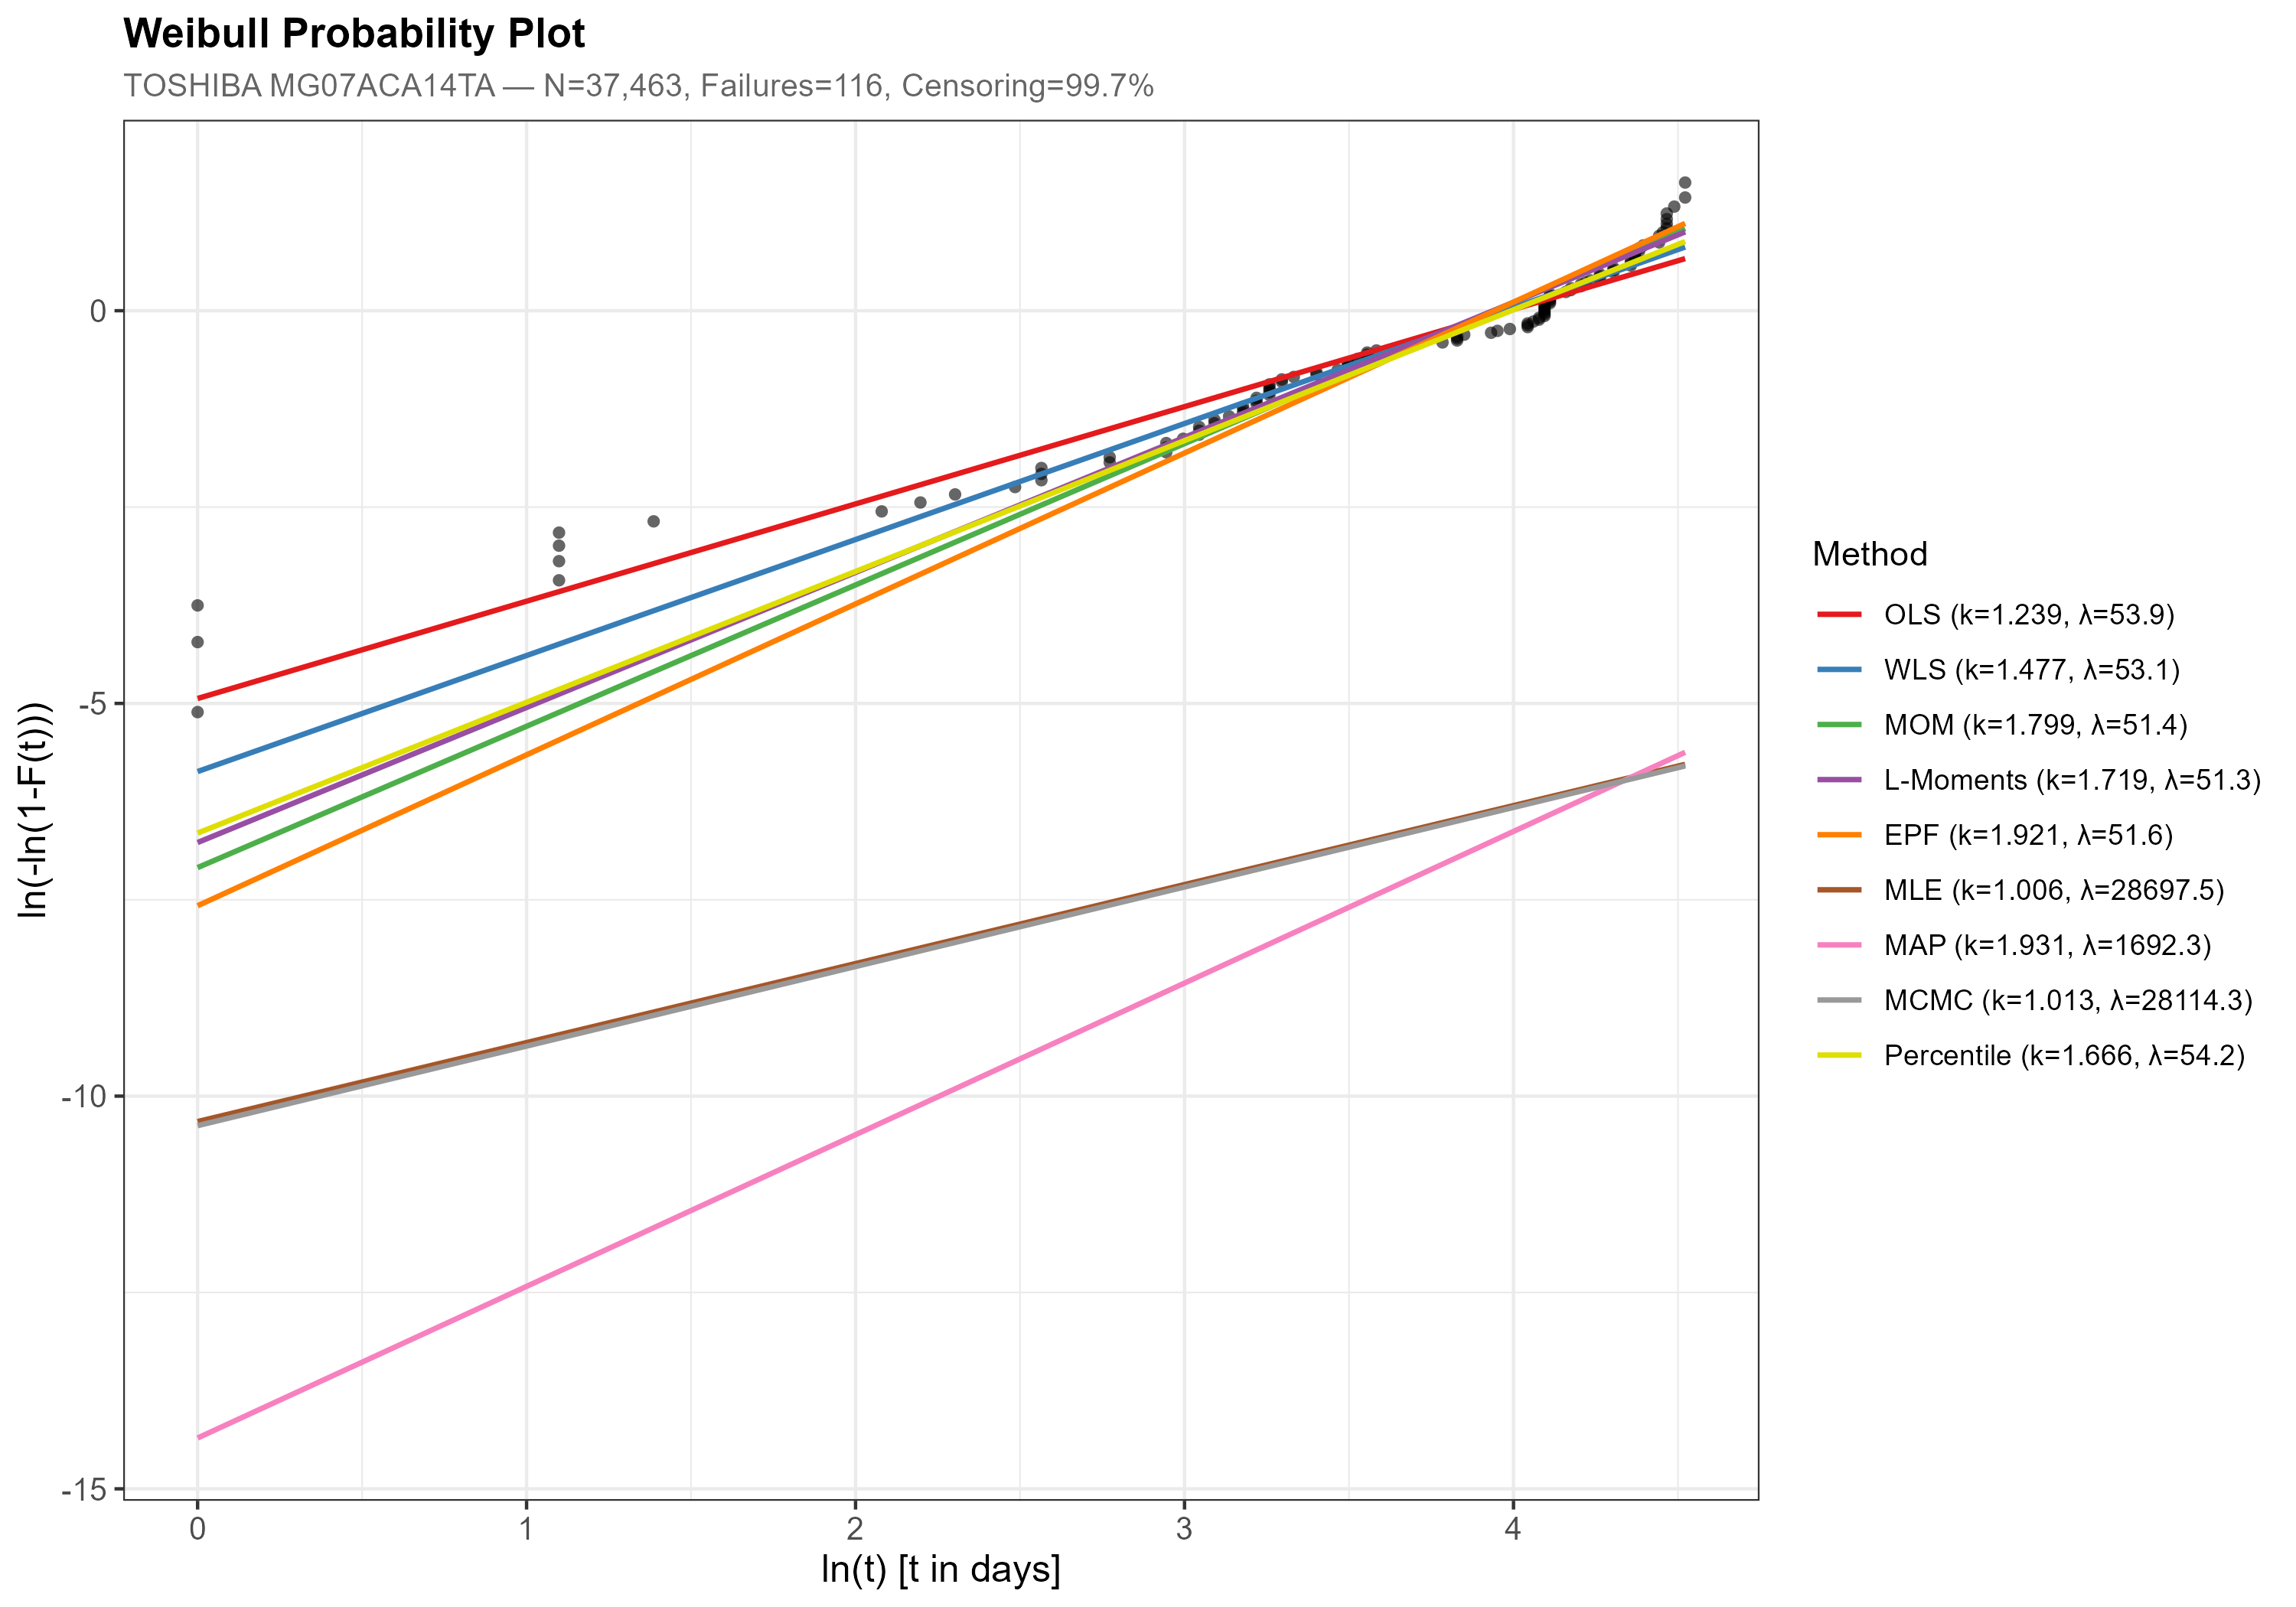
\includegraphics[width=0.95\linewidth]{results/plots/plot1_weibull_probability_TOSHIBA_MG07ACA14TA.png}
\caption{plot1 weibull probability — TOSHIBA MG07ACA14TA}
\end{figure}

\begin{figure}[H]
\centering
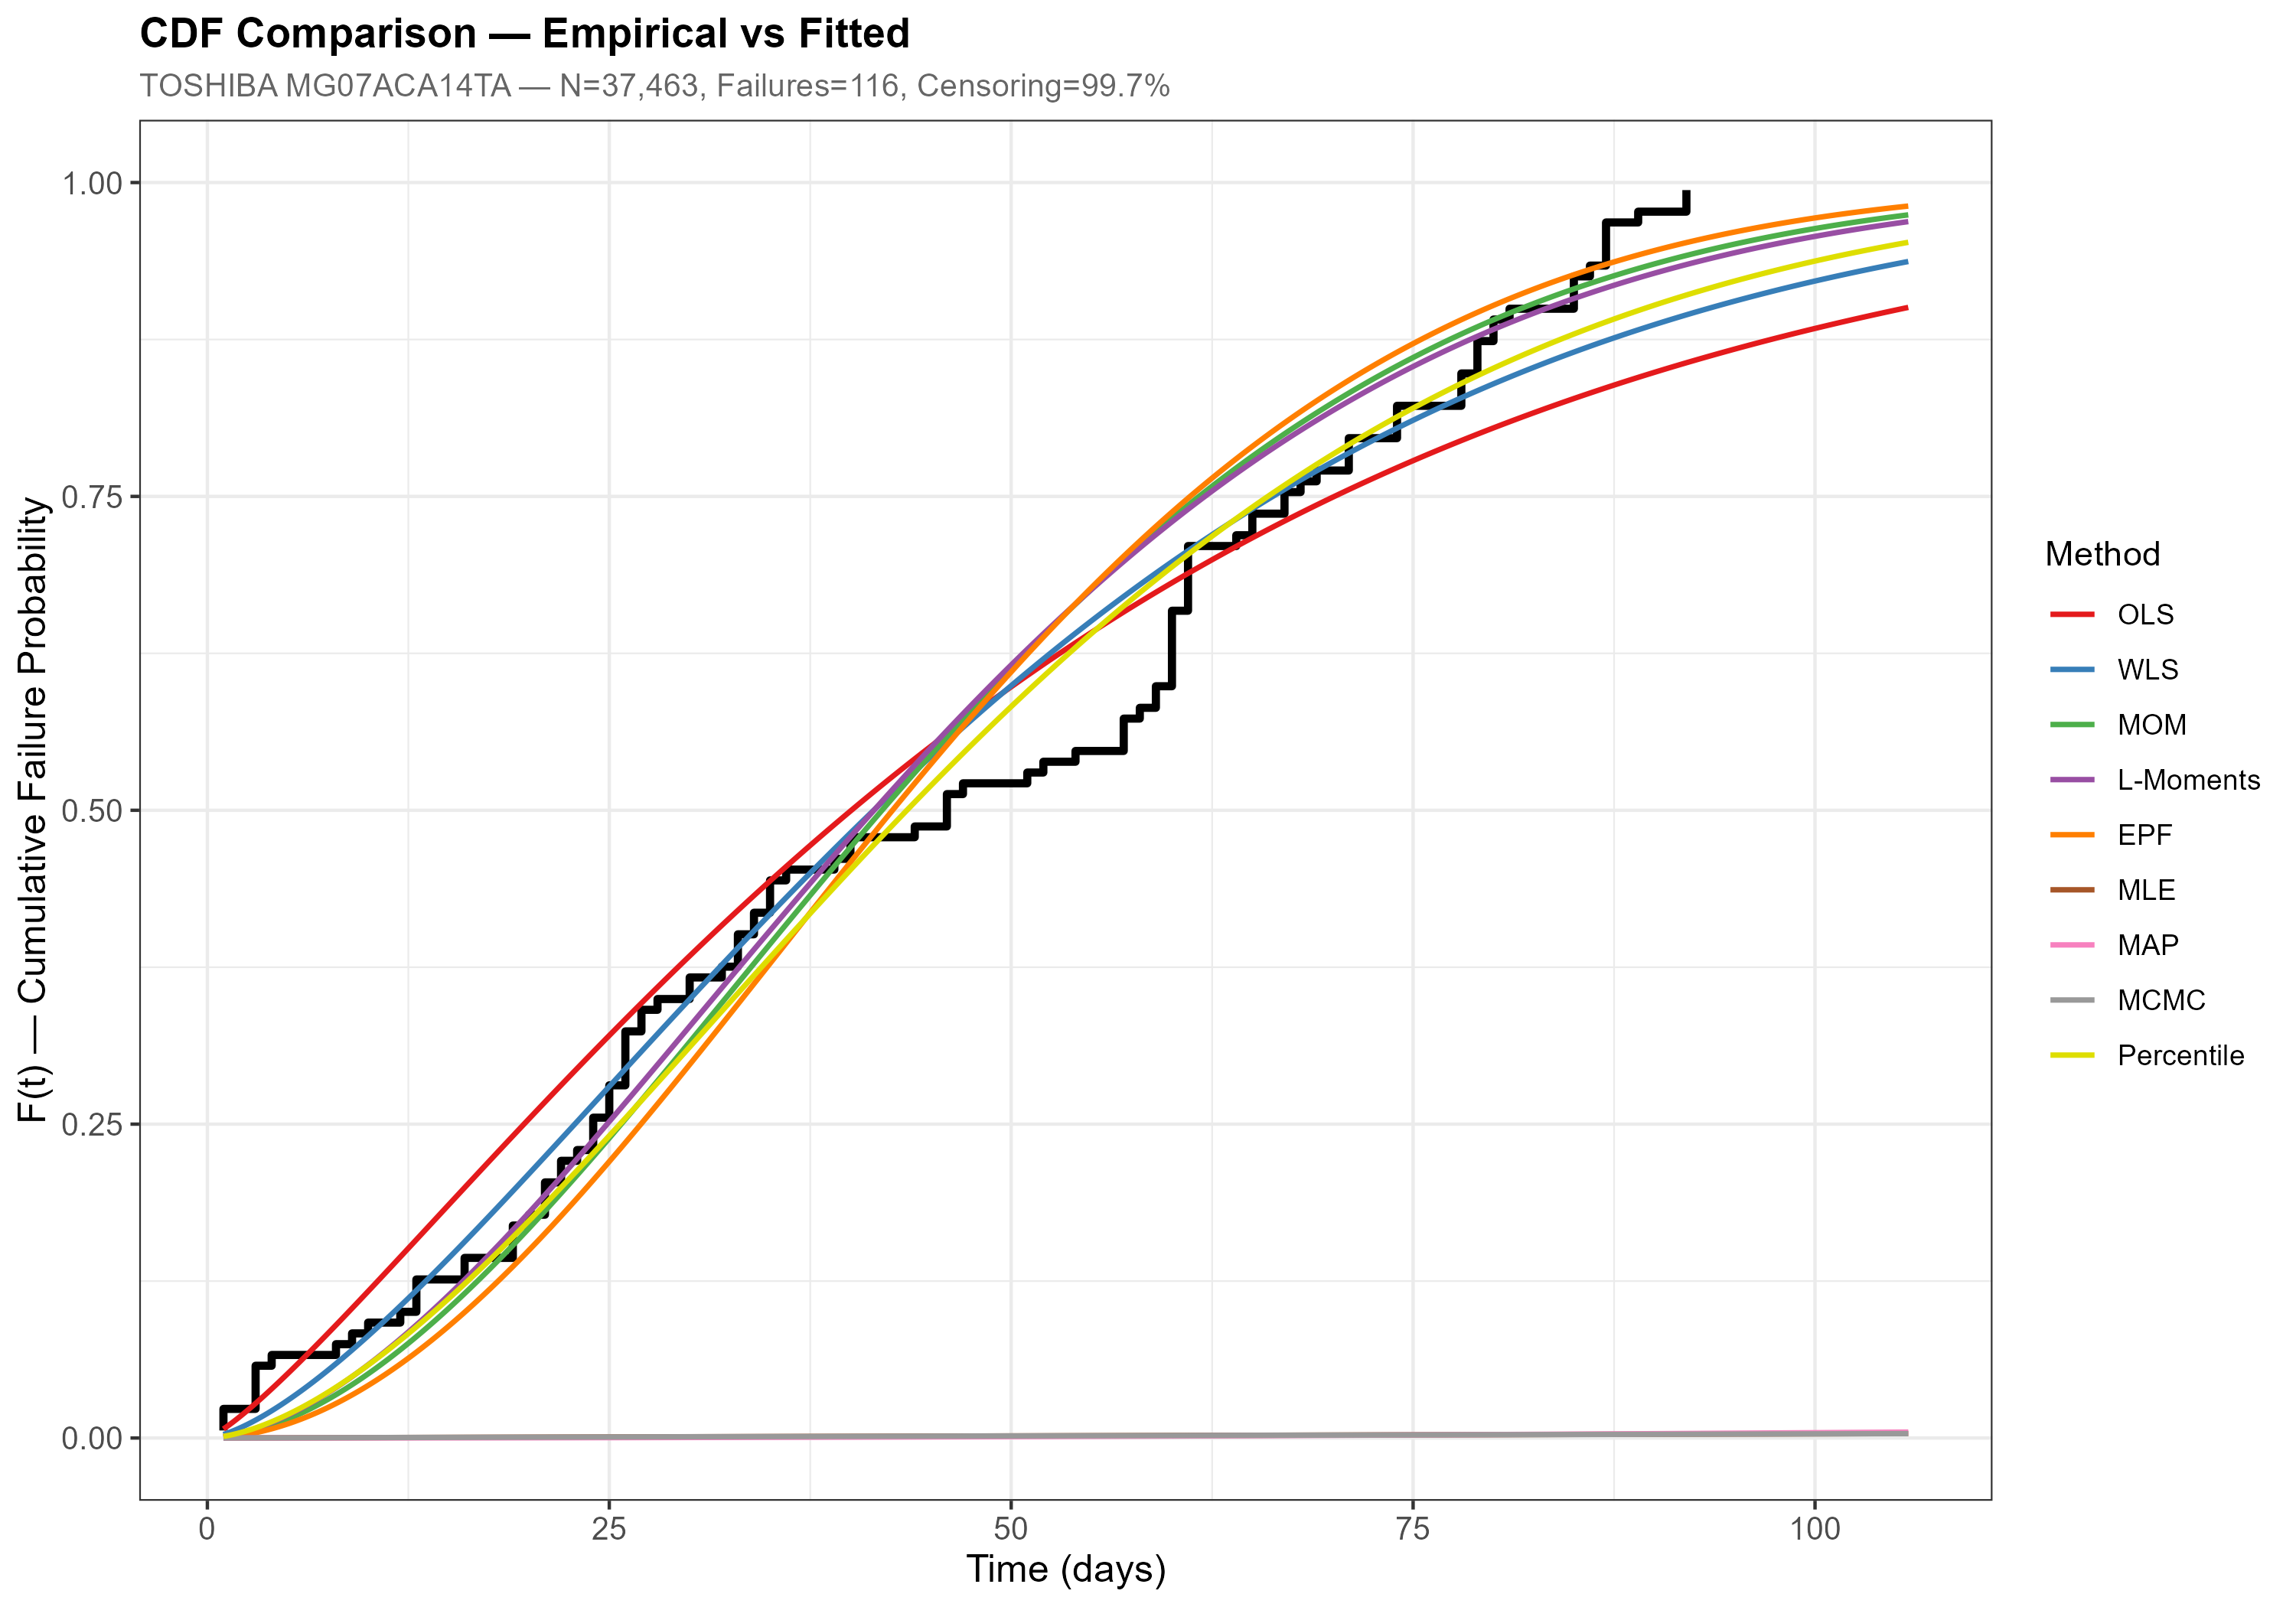
\includegraphics[width=0.95\linewidth]{results/plots/plot2_cdf_TOSHIBA_MG07ACA14TA.png}
\caption{plot2 cdf — TOSHIBA MG07ACA14TA}
\end{figure}

\begin{figure}[H]
\centering
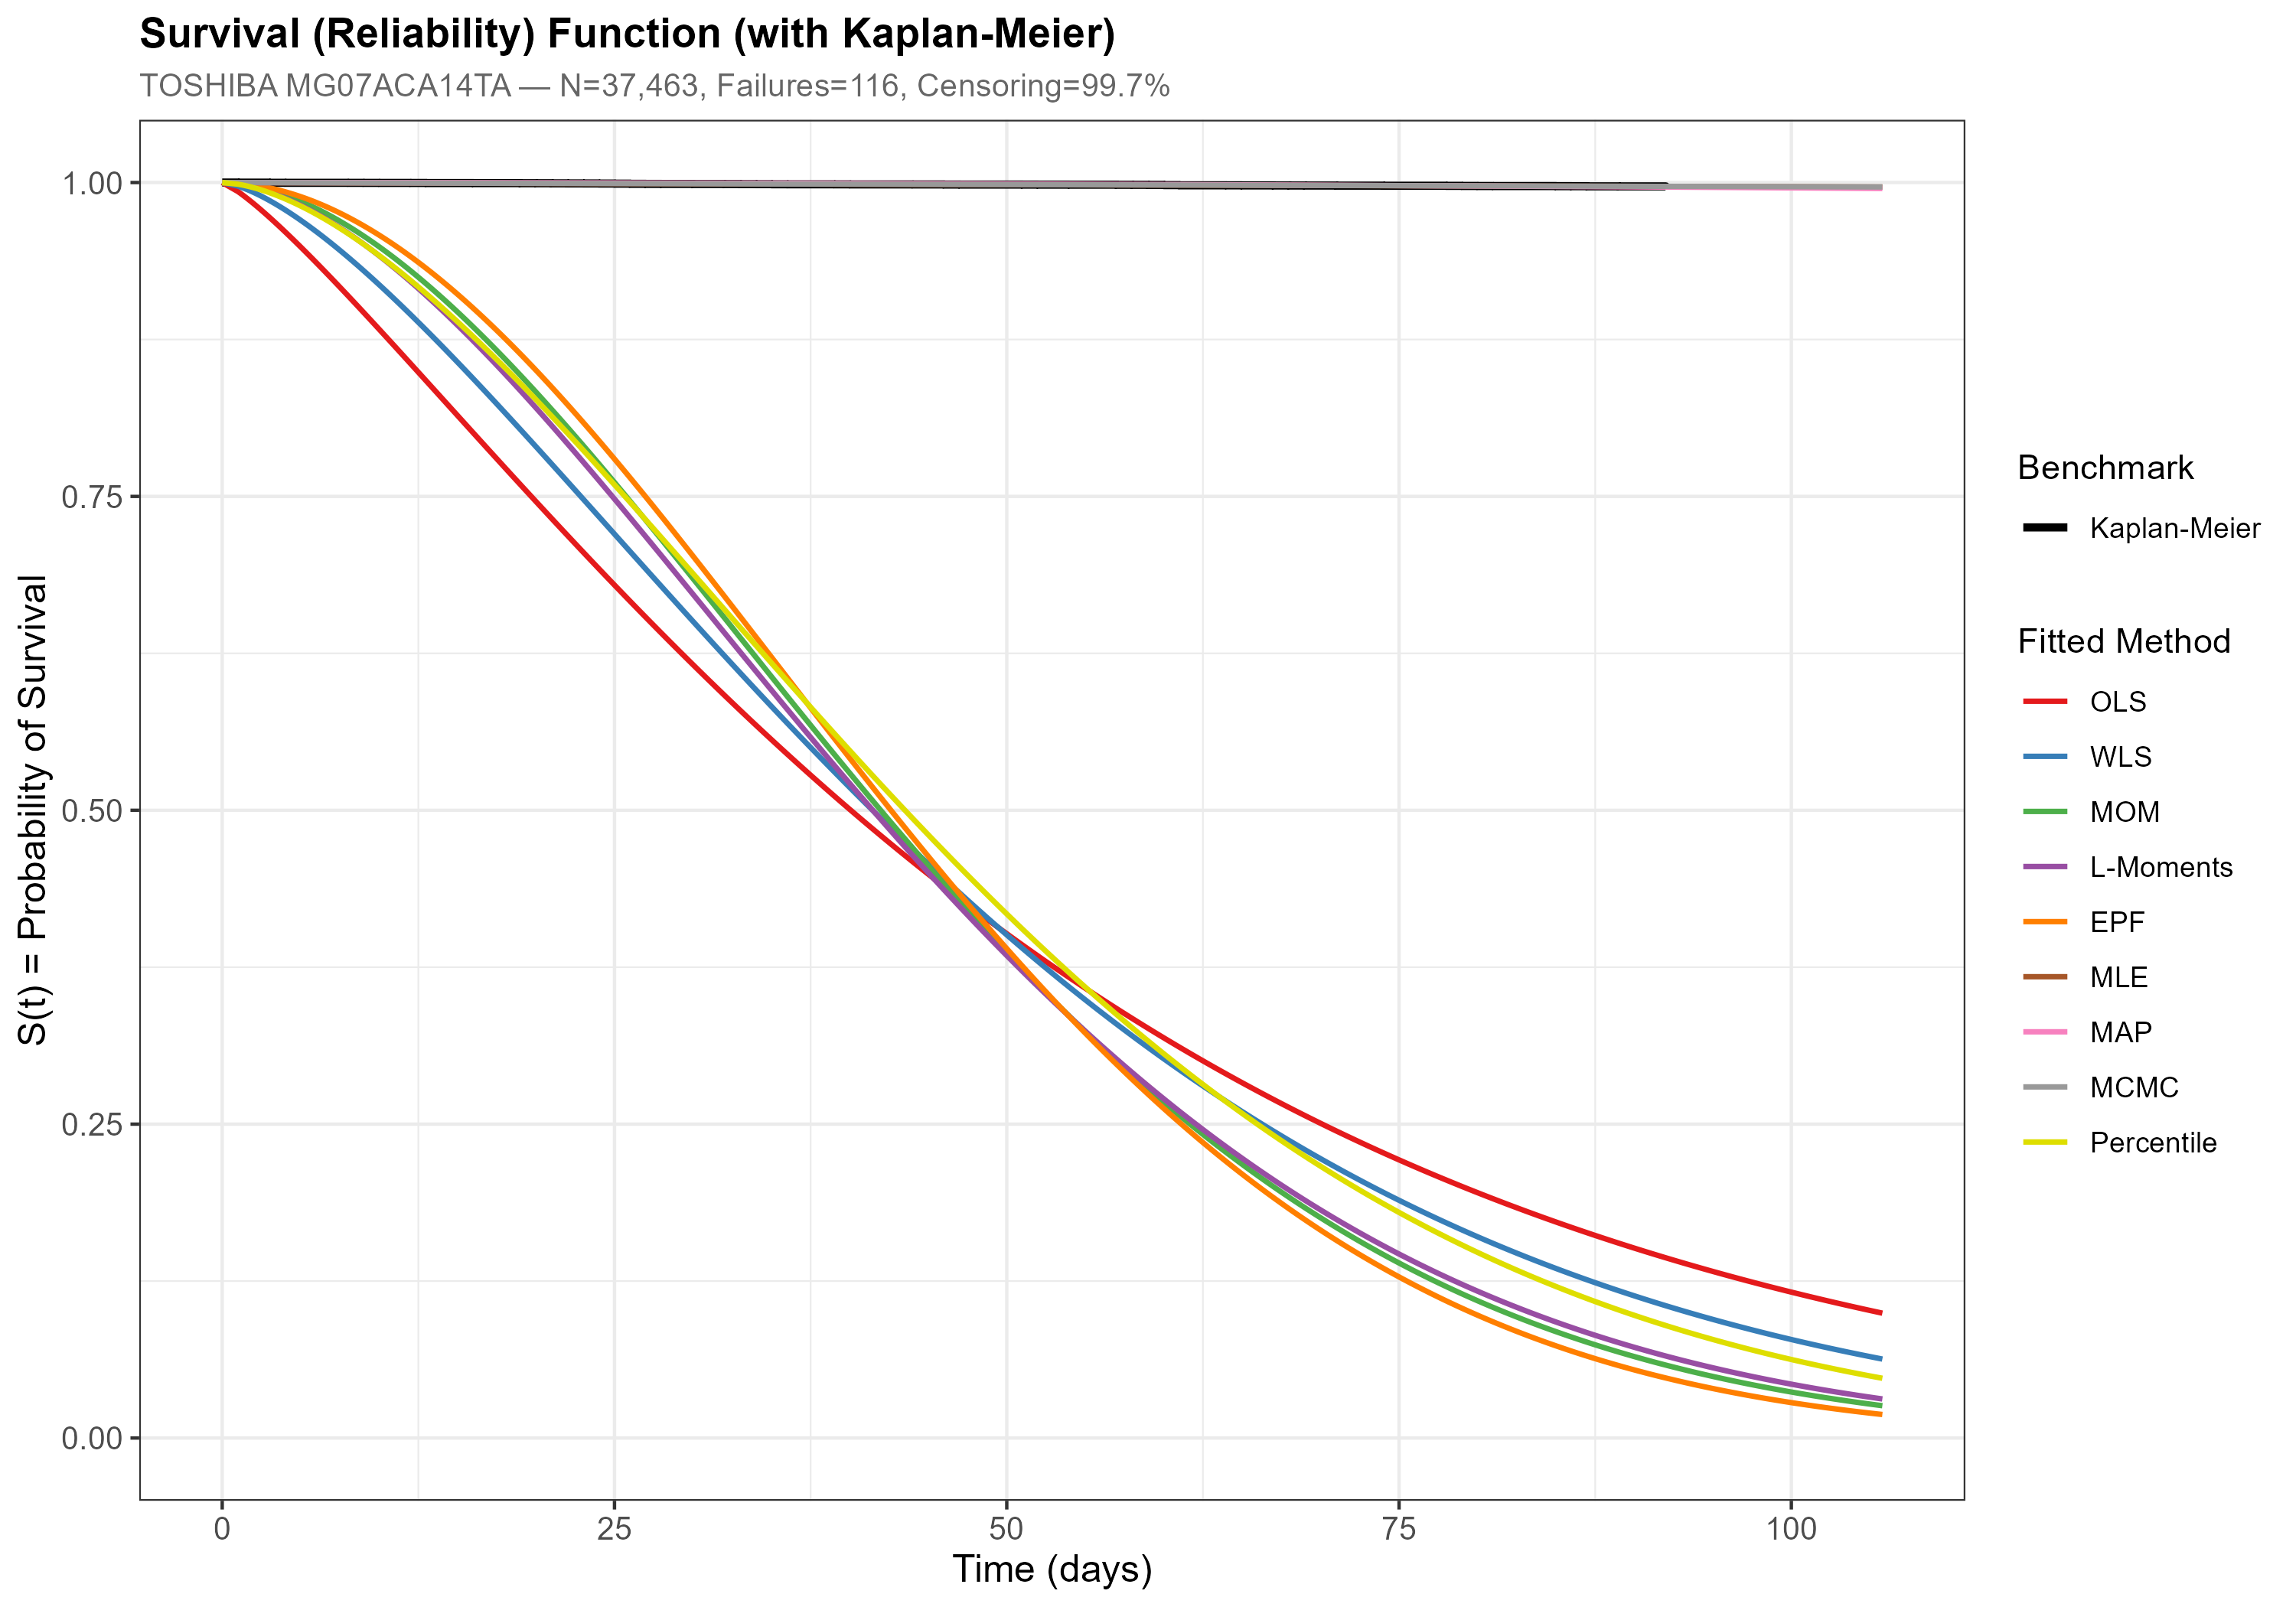
\includegraphics[width=0.95\linewidth]{results/plots/plot3_survival_TOSHIBA_MG07ACA14TA.png}
\caption{plot3 survival — TOSHIBA MG07ACA14TA}
\end{figure}

\begin{figure}[H]
\centering
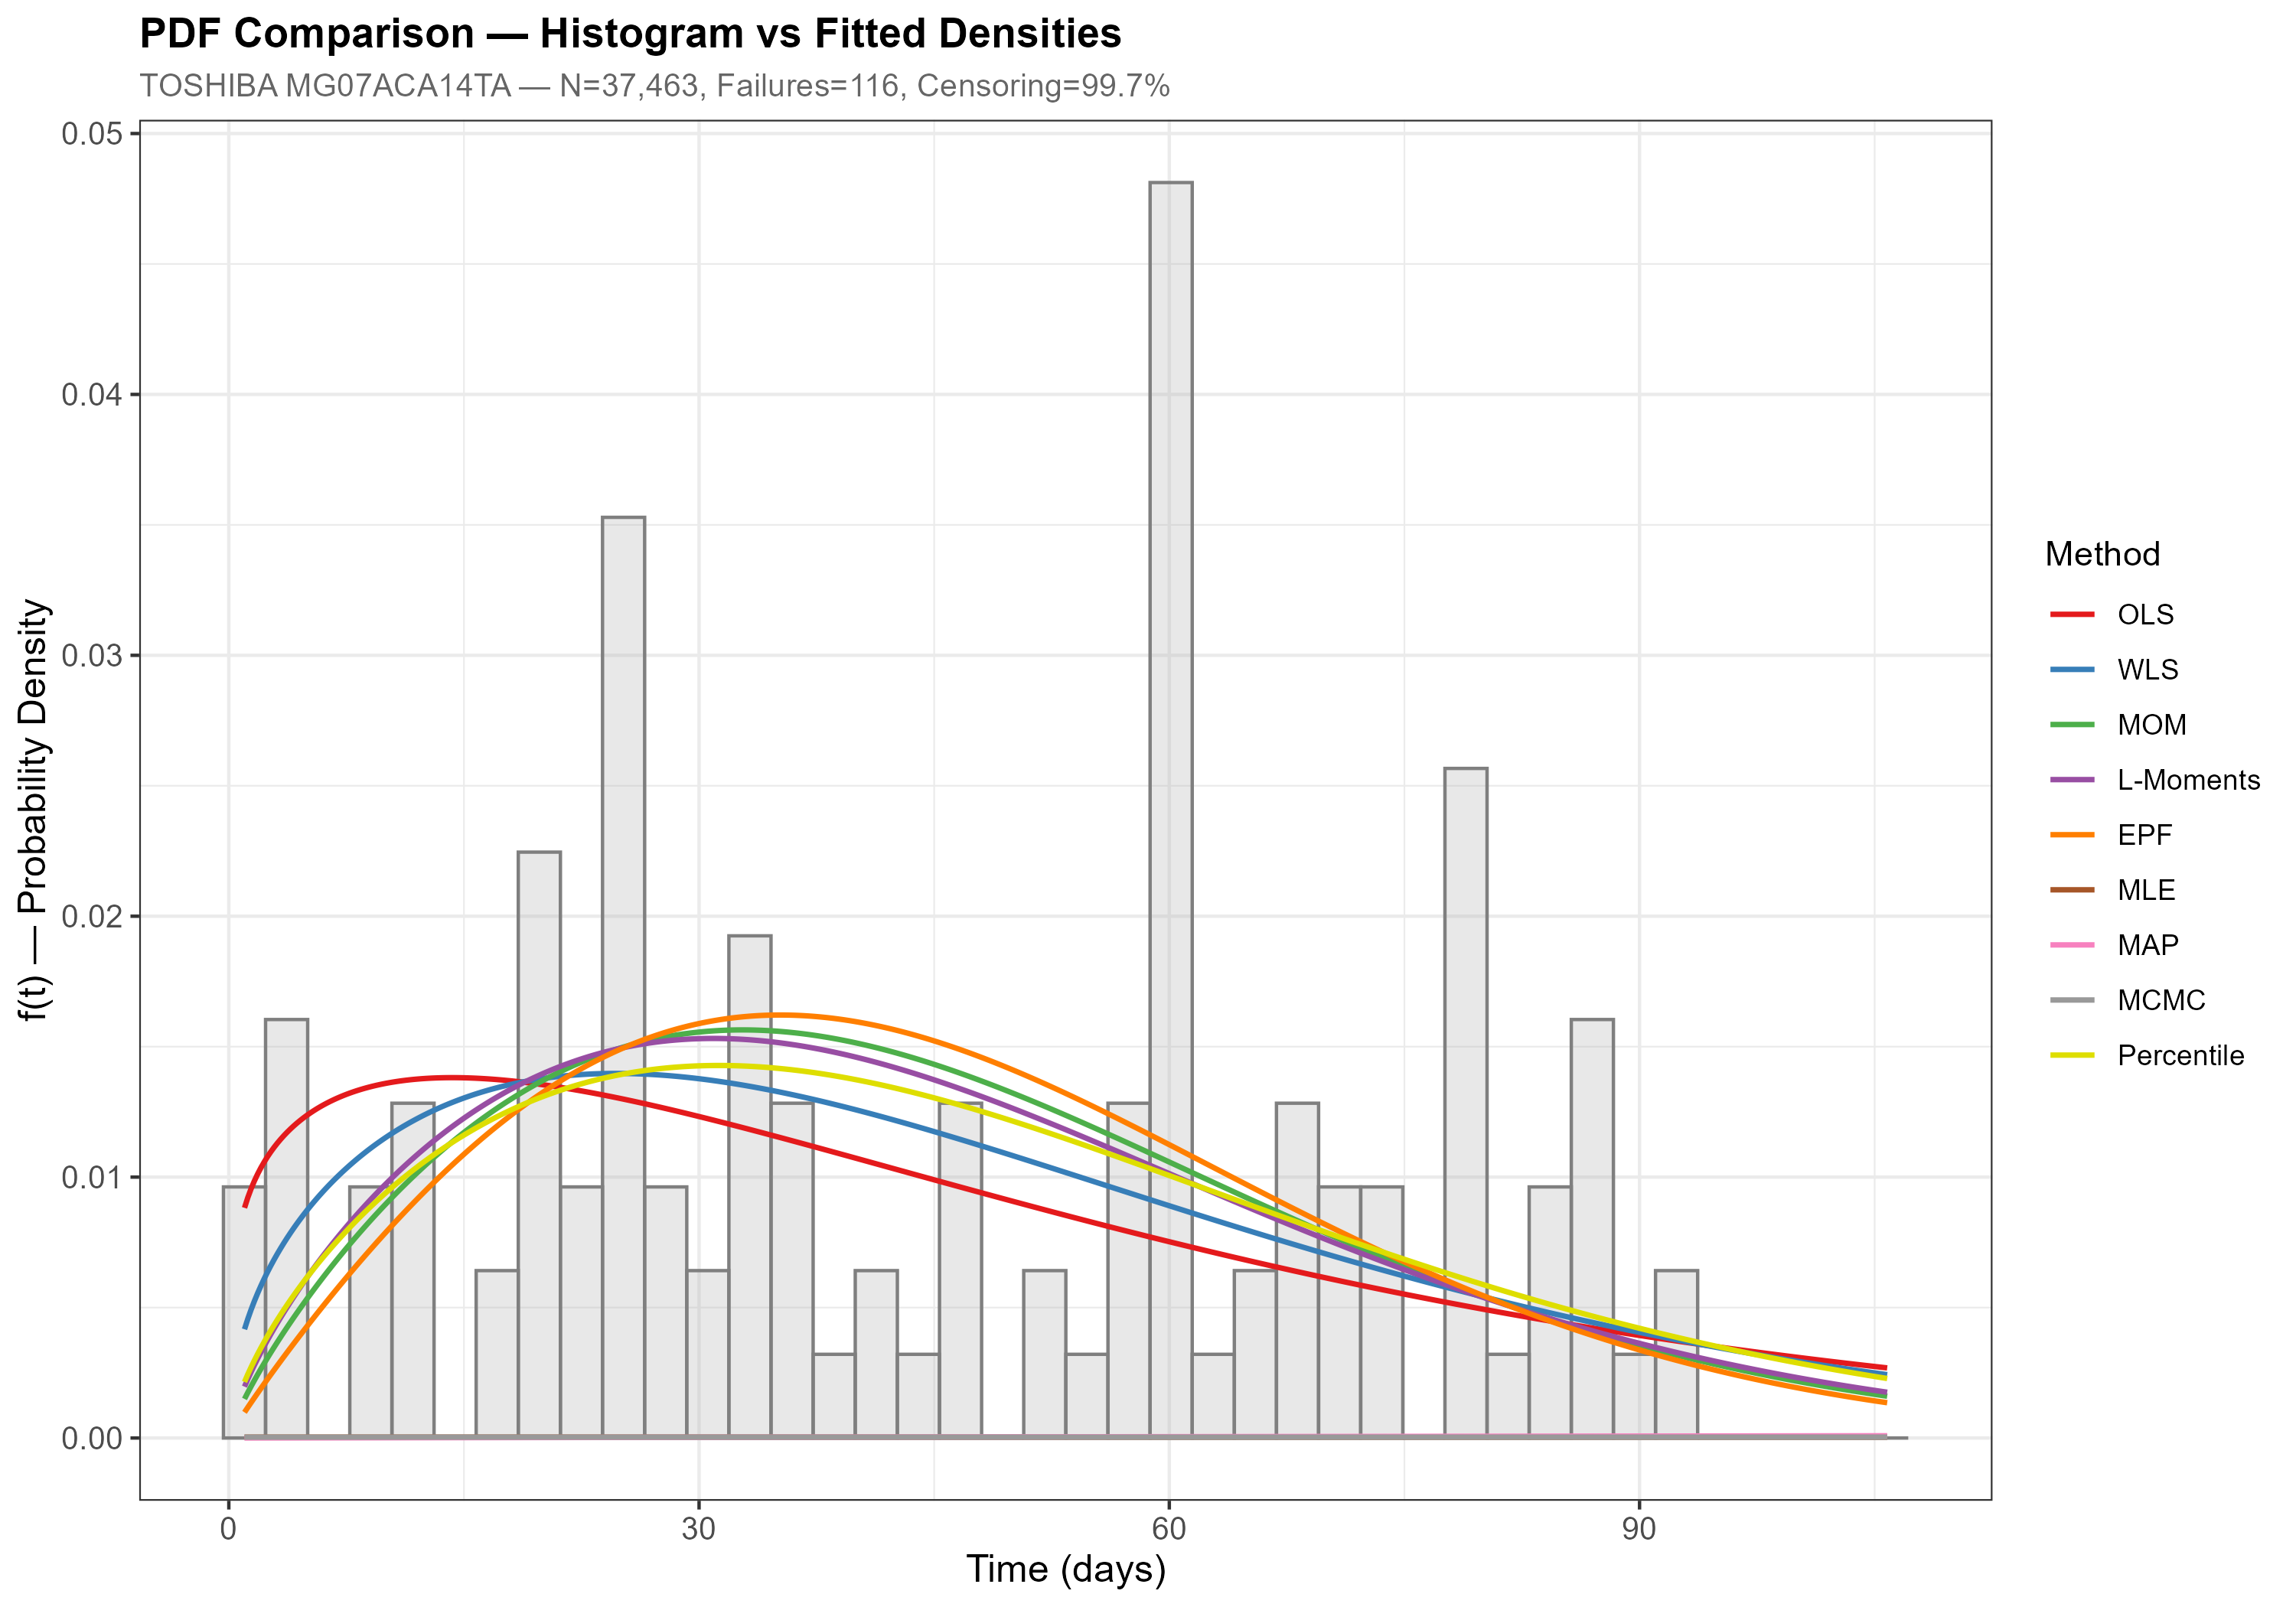
\includegraphics[width=0.95\linewidth]{results/plots/plot4_pdf_TOSHIBA_MG07ACA14TA.png}
\caption{plot4 pdf — TOSHIBA MG07ACA14TA}
\end{figure}

\begin{figure}[H]
\centering
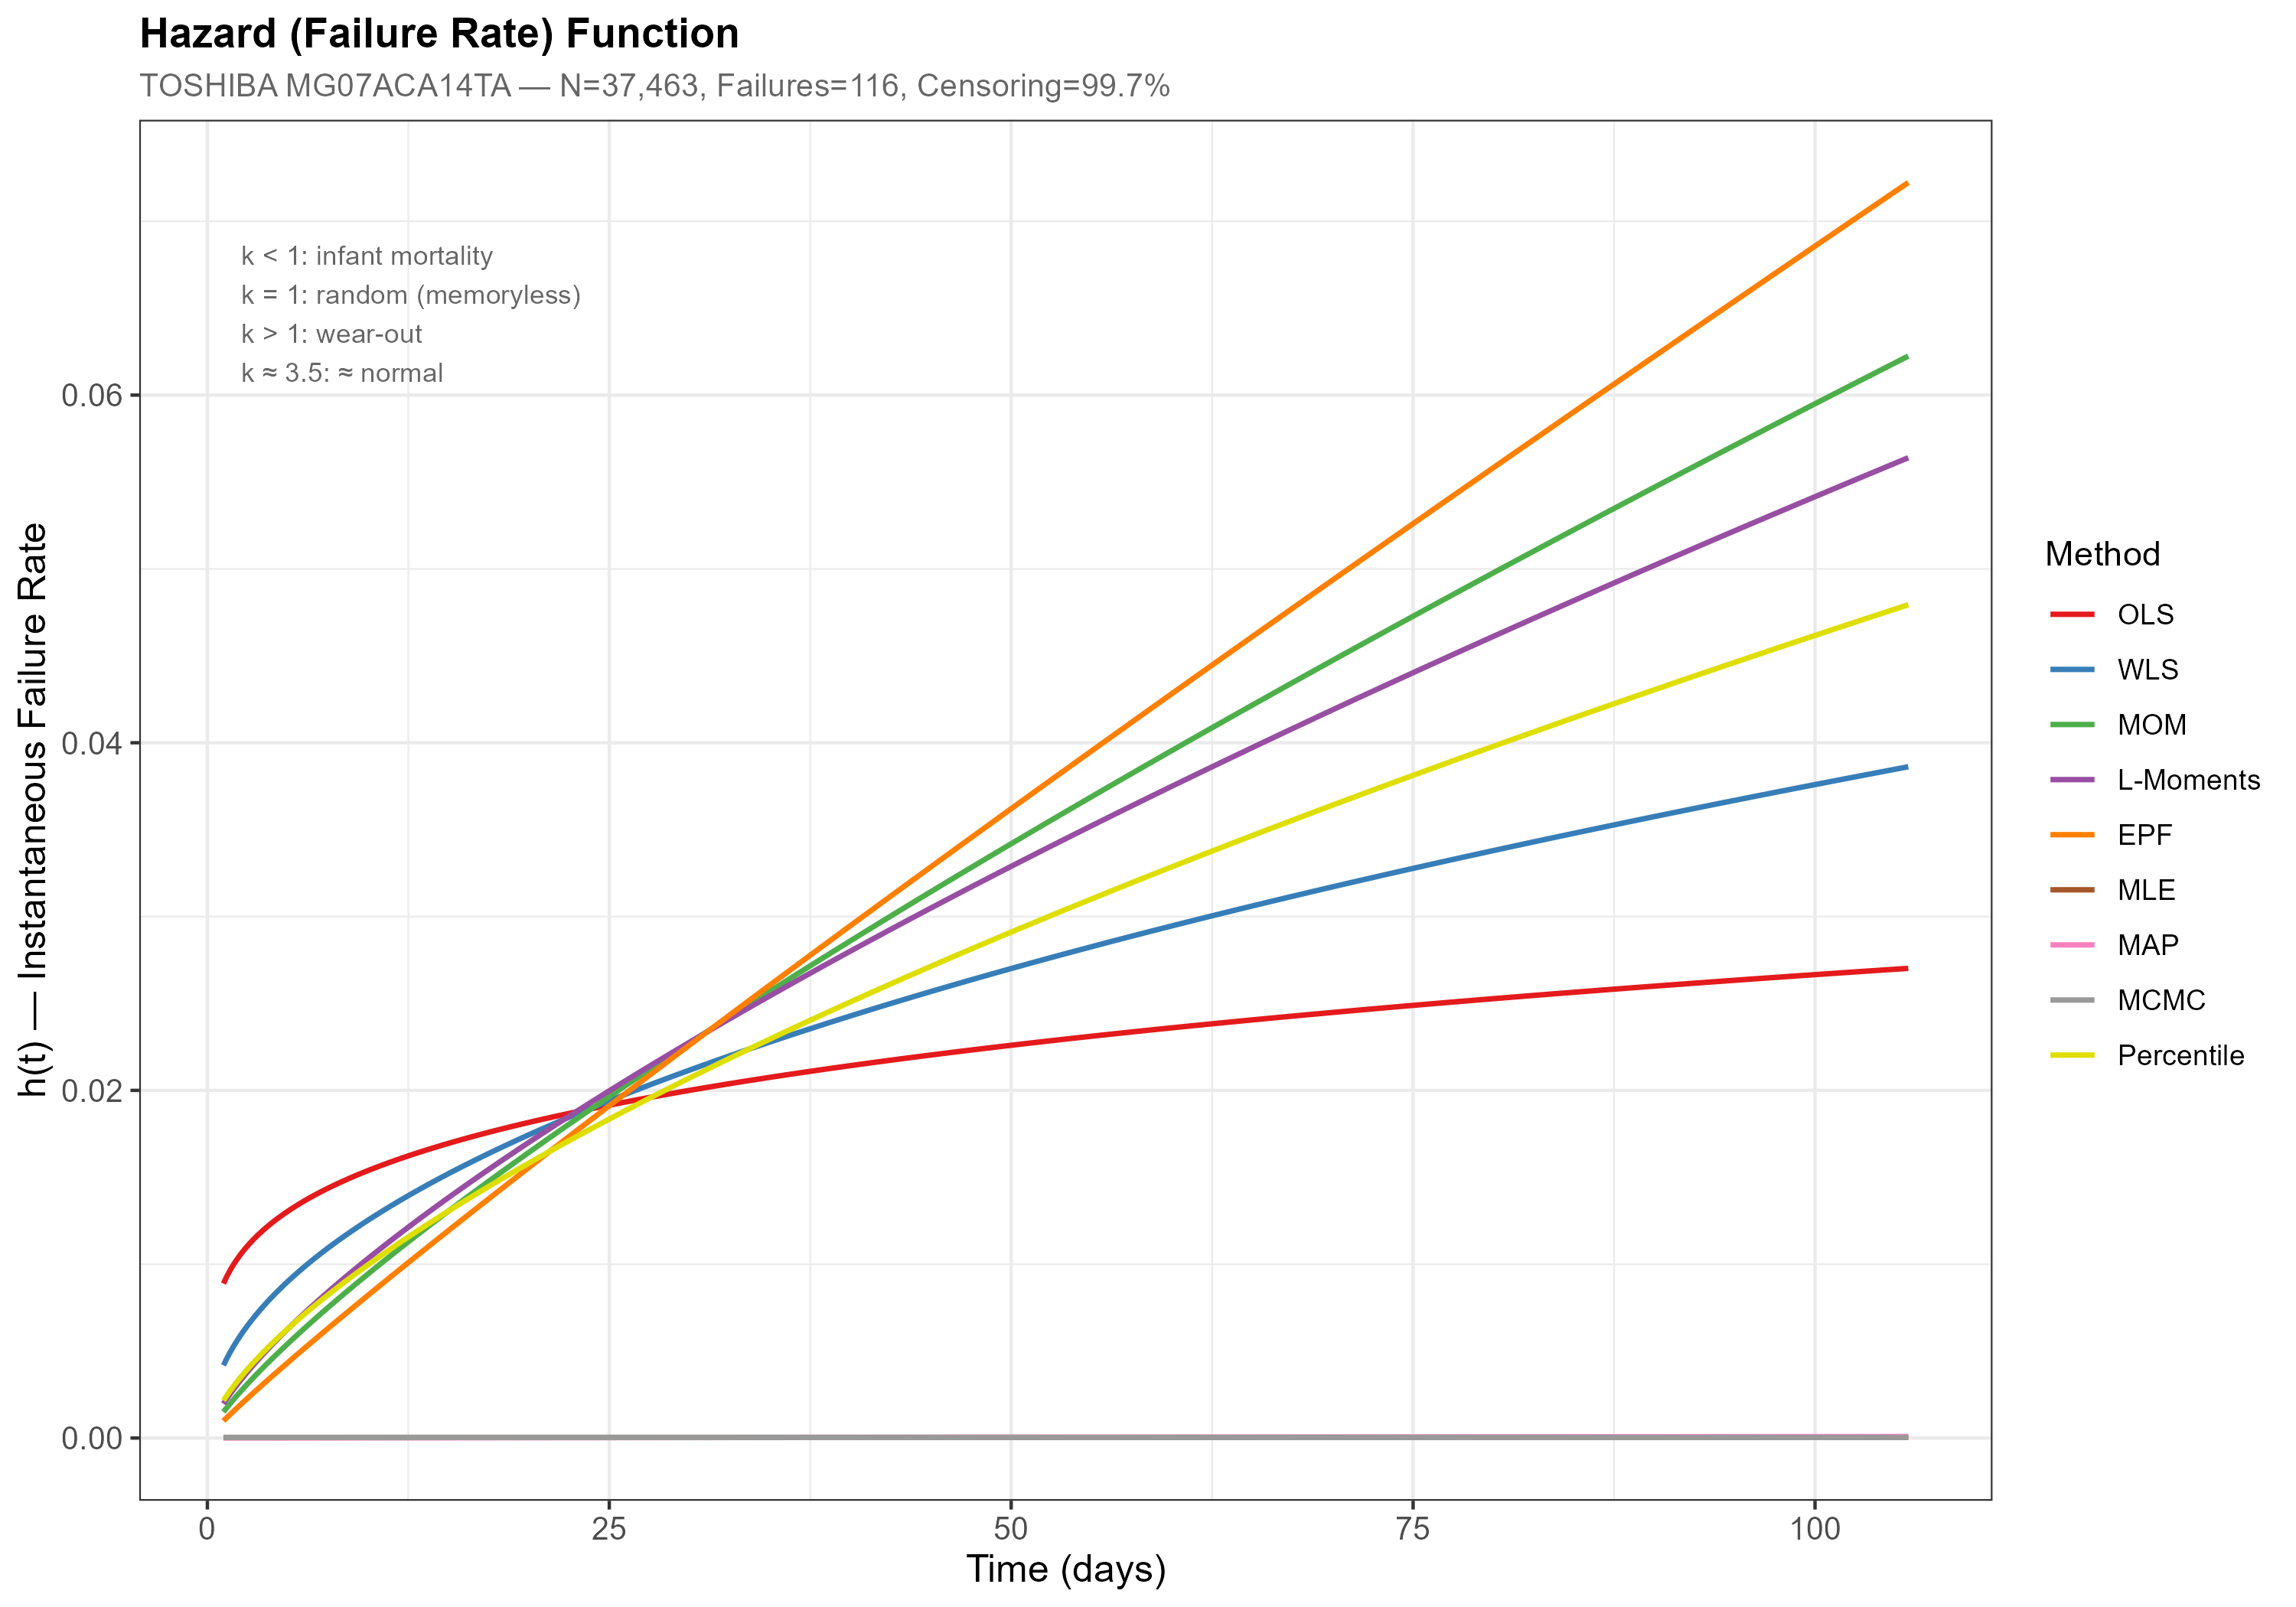
\includegraphics[width=0.95\linewidth]{results/plots/plot5_hazard_TOSHIBA_MG07ACA14TA.png}
\caption{plot5 hazard — TOSHIBA MG07ACA14TA}
\end{figure}

\begin{figure}[H]
\centering
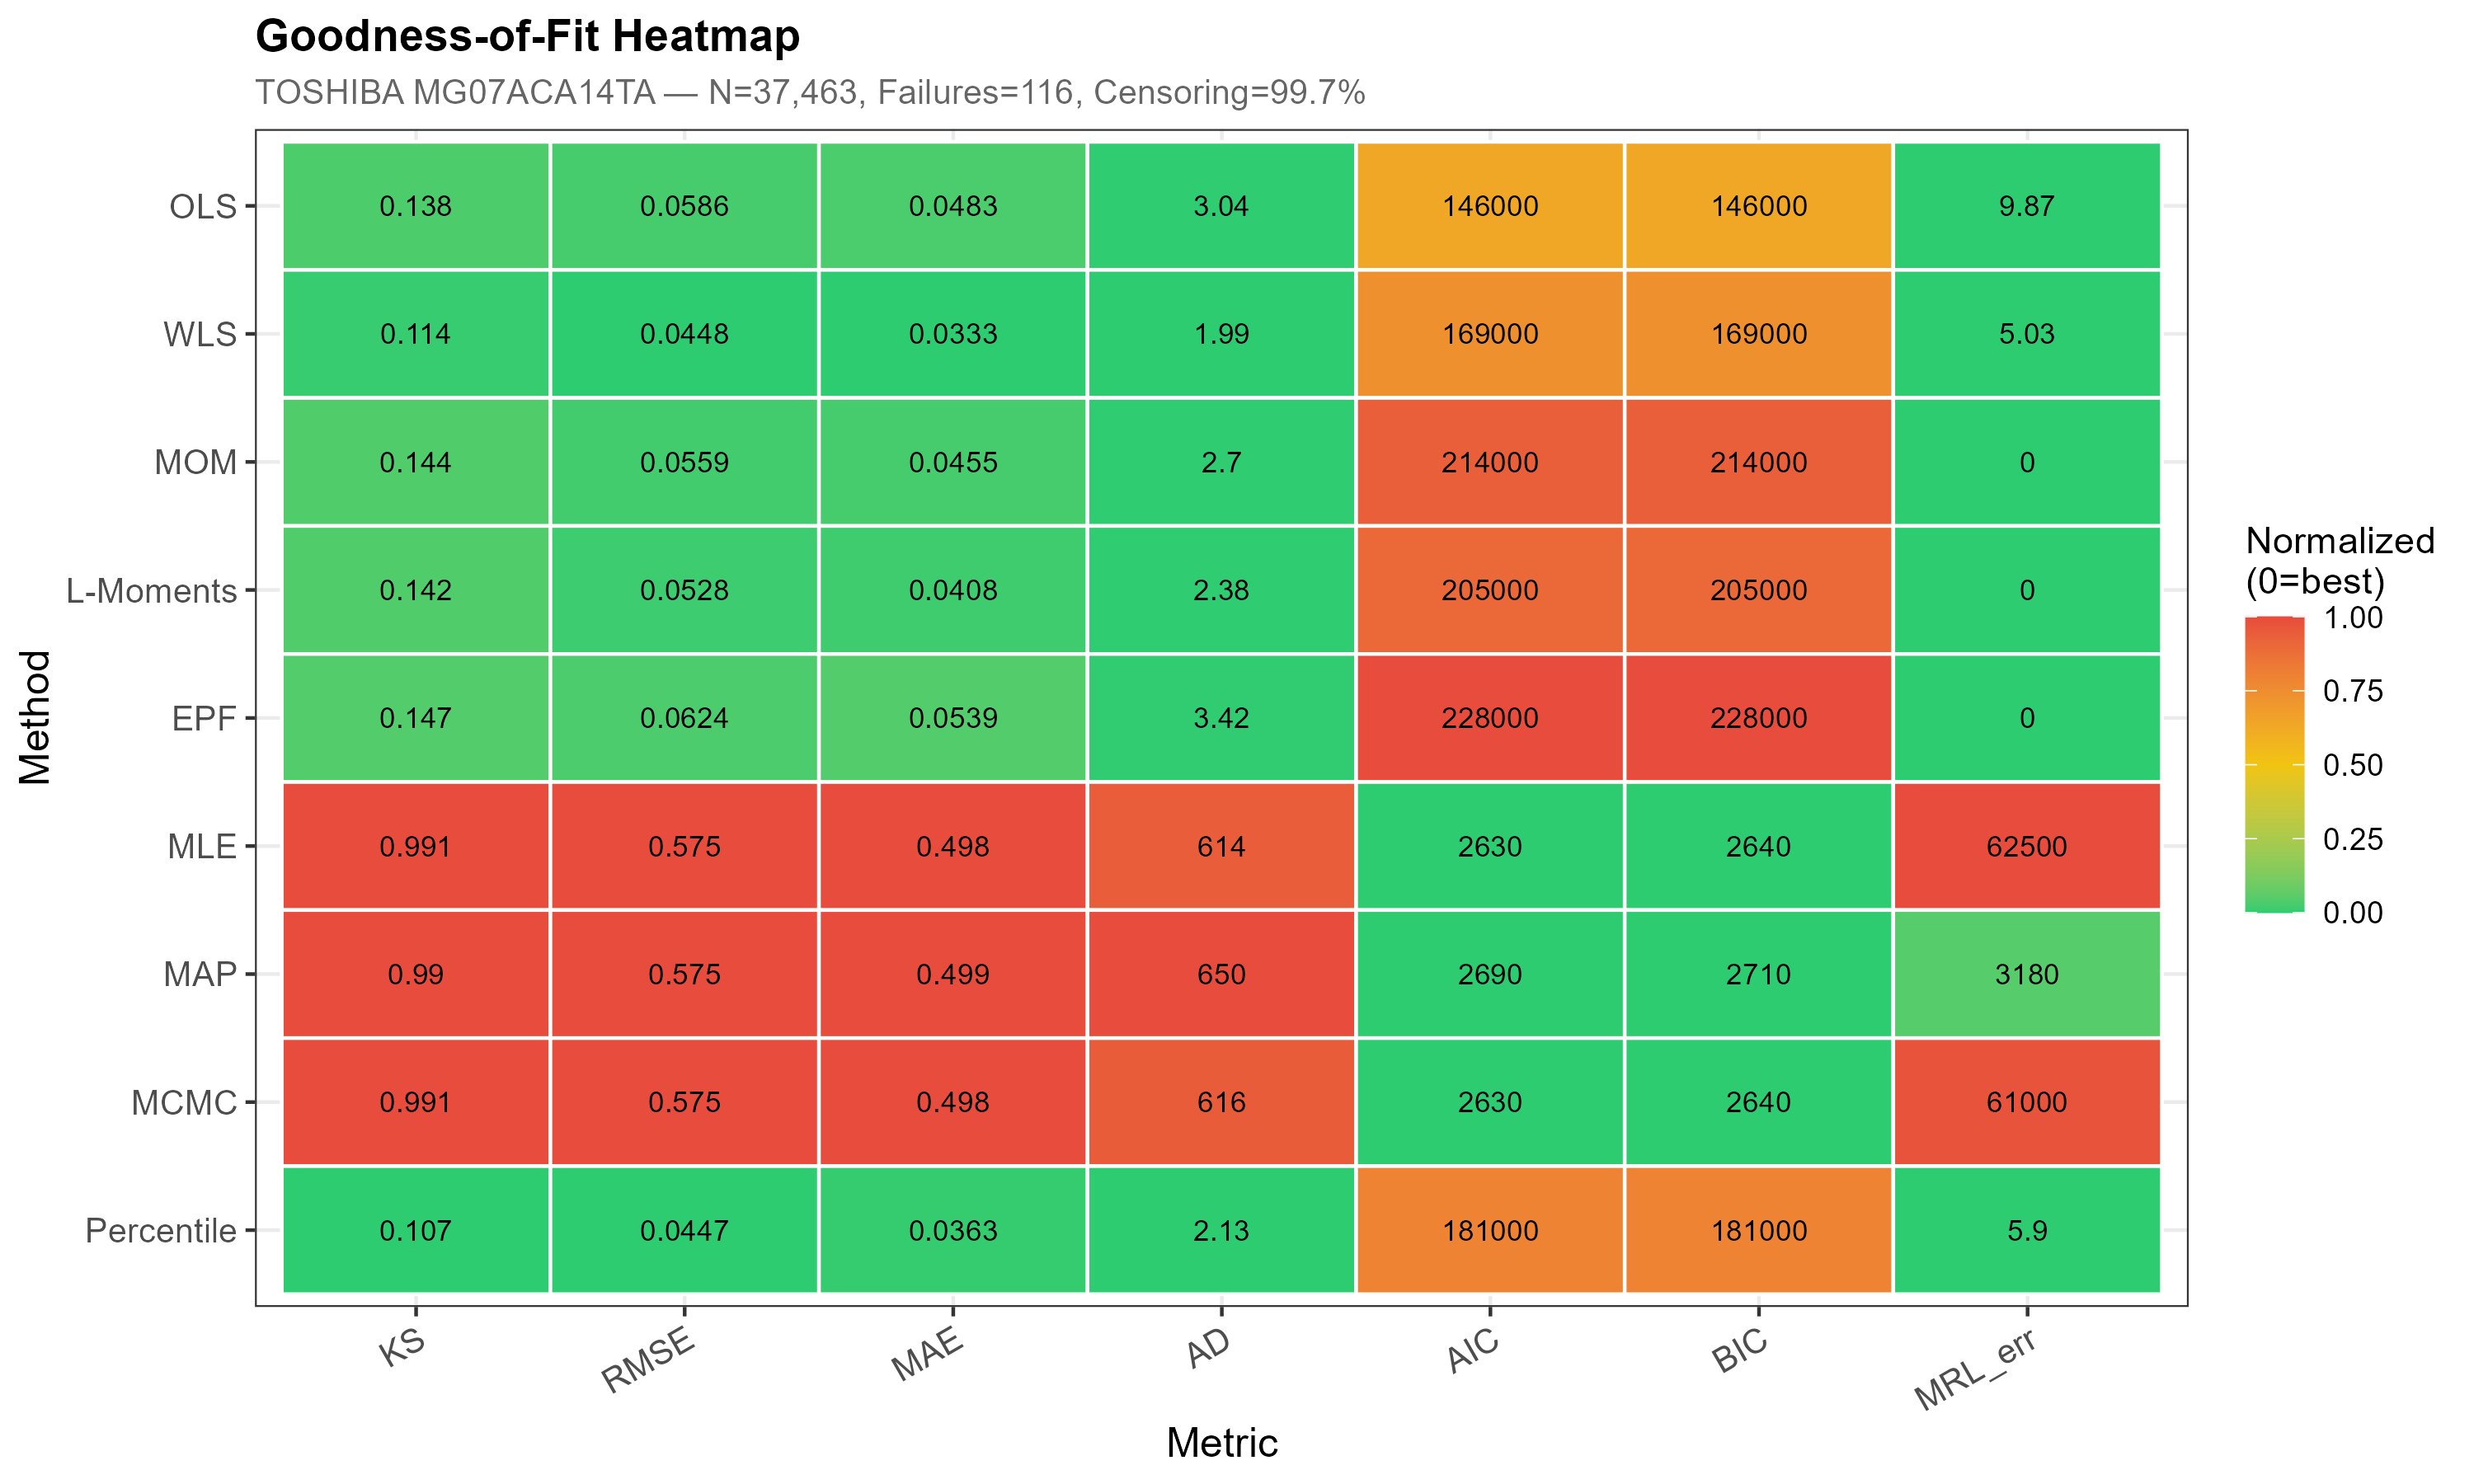
\includegraphics[width=0.95\linewidth]{results/plots/plot6_gof_heatmap_TOSHIBA_MG07ACA14TA.png}
\caption{plot6 gof heatmap — TOSHIBA MG07ACA14TA}
\end{figure}

\begin{figure}[H]
\centering
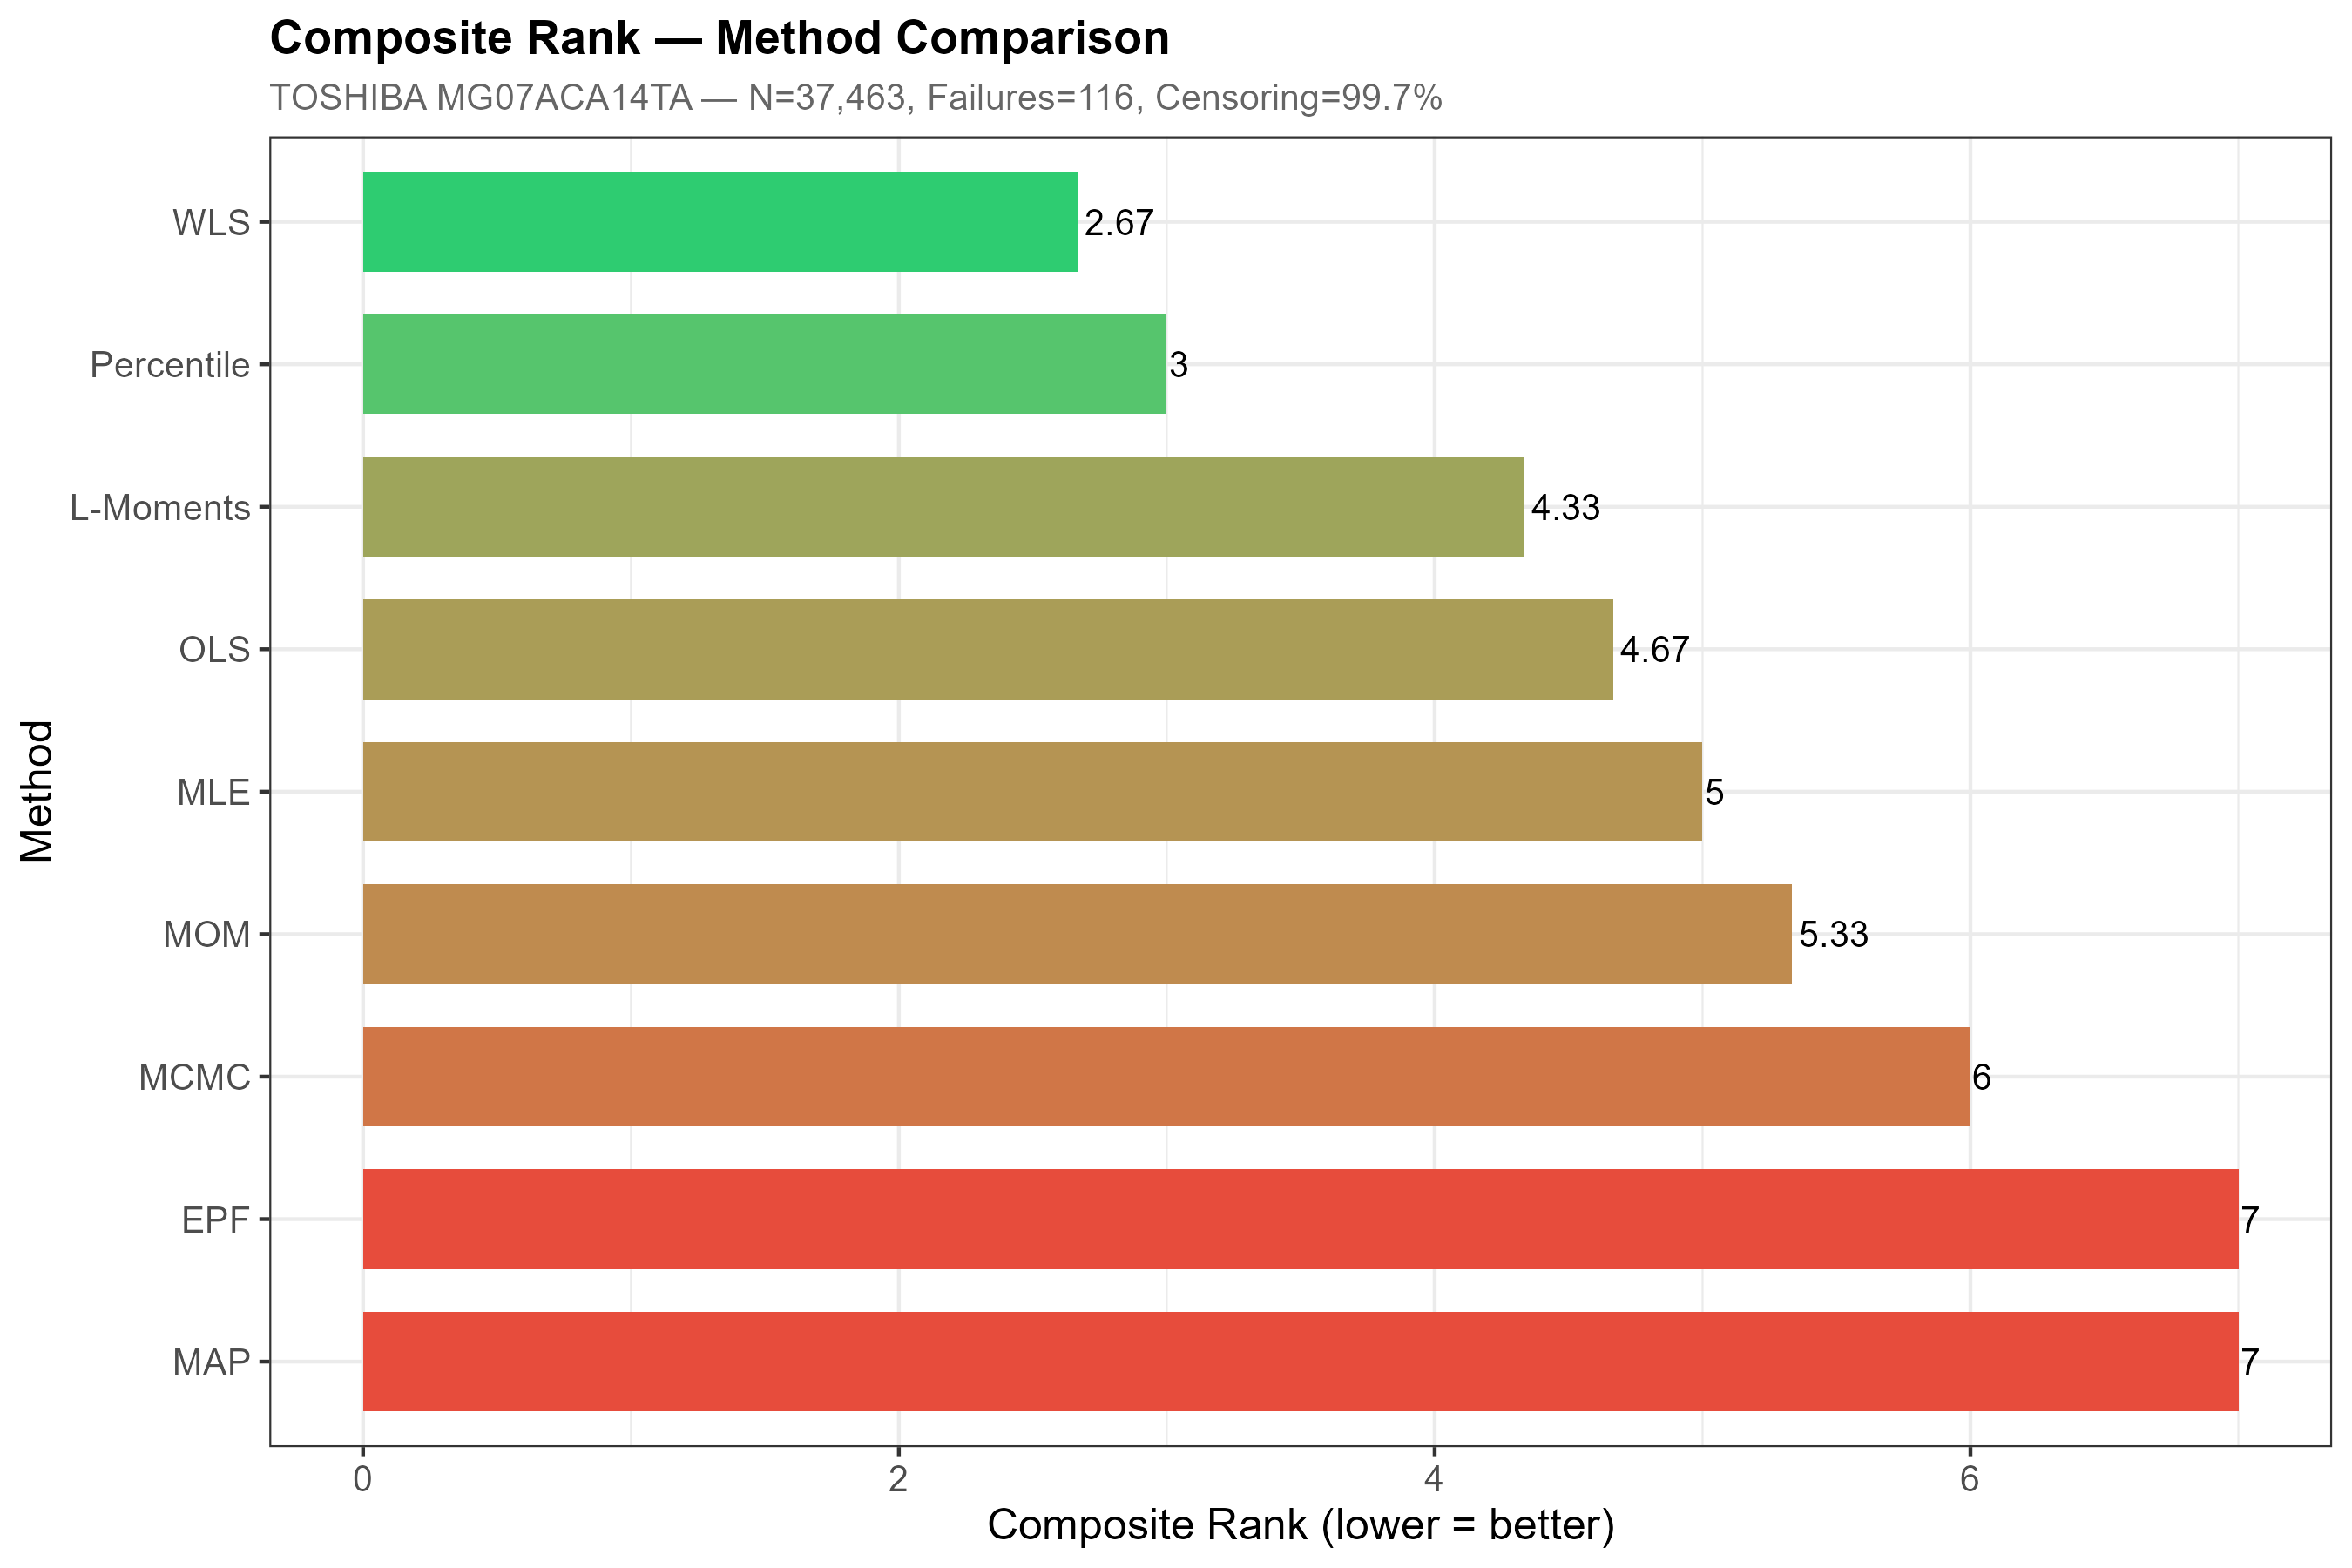
\includegraphics[width=0.95\linewidth]{results/plots/plot7_composite_rank_TOSHIBA_MG07ACA14TA.png}
\caption{plot7 composite rank — TOSHIBA MG07ACA14TA}
\end{figure}

\begin{figure}[H]
\centering
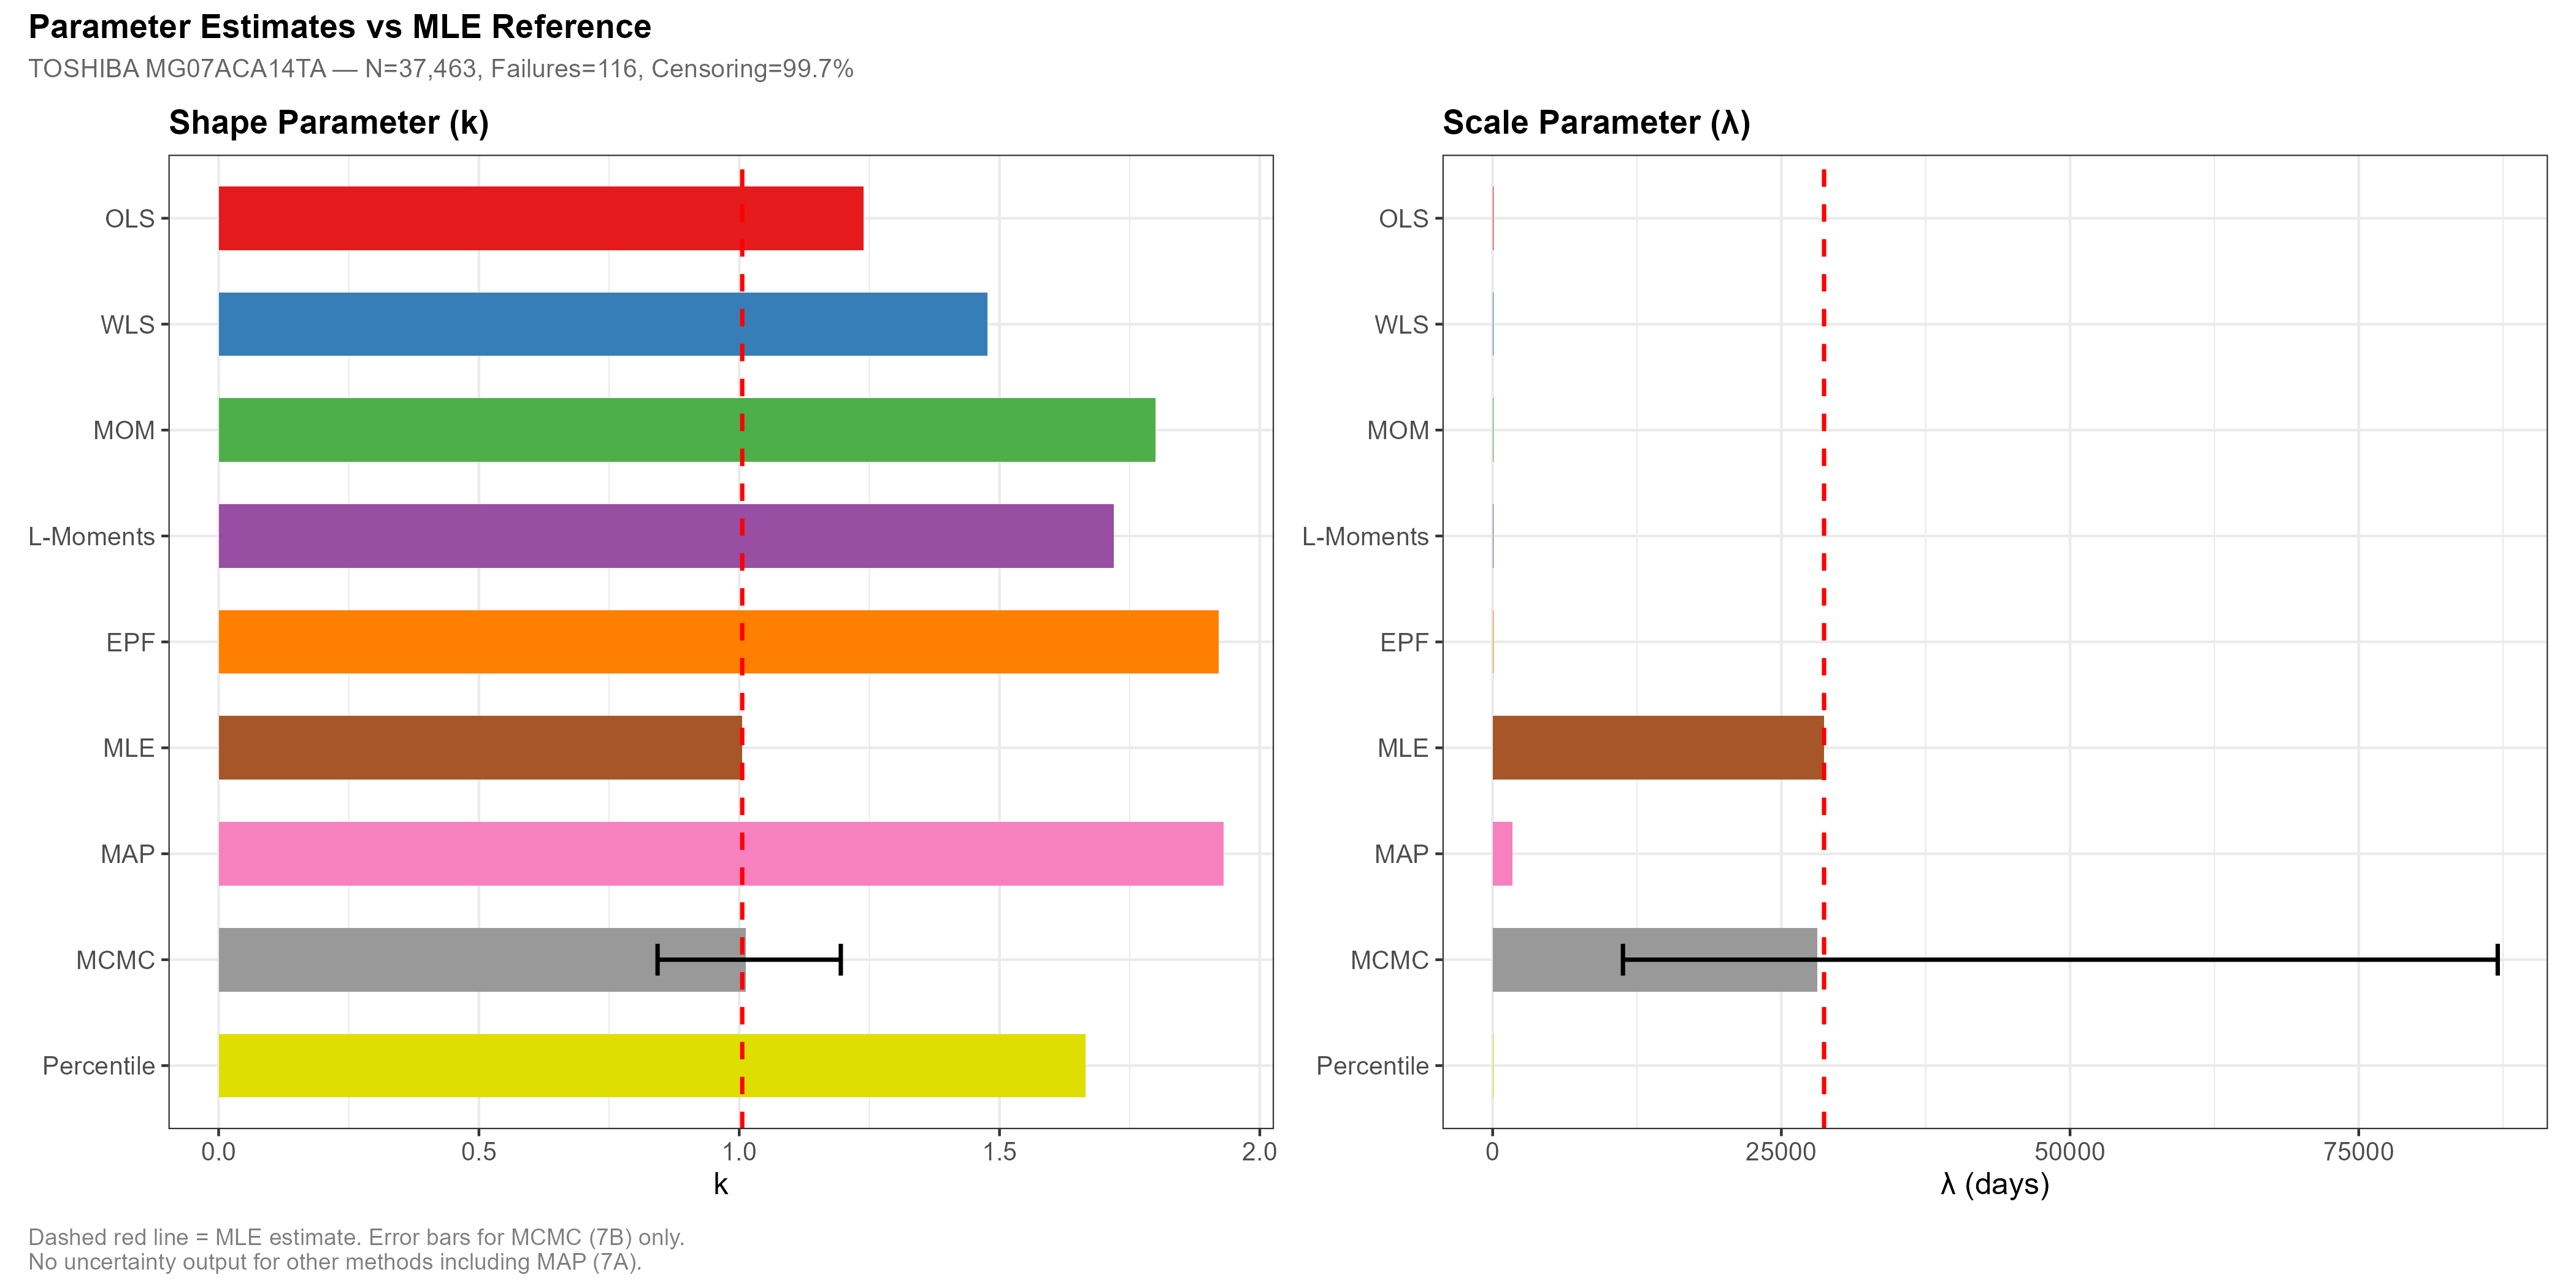
\includegraphics[width=0.95\linewidth]{results/plots/plot8_parameters_TOSHIBA_MG07ACA14TA.png}
\caption{plot8 parameters — TOSHIBA MG07ACA14TA}
\end{figure}

\subsection{TOSHIBA MG08ACA16TA}\label{toshiba-mg08aca16ta}

\begin{figure}[H]
\centering
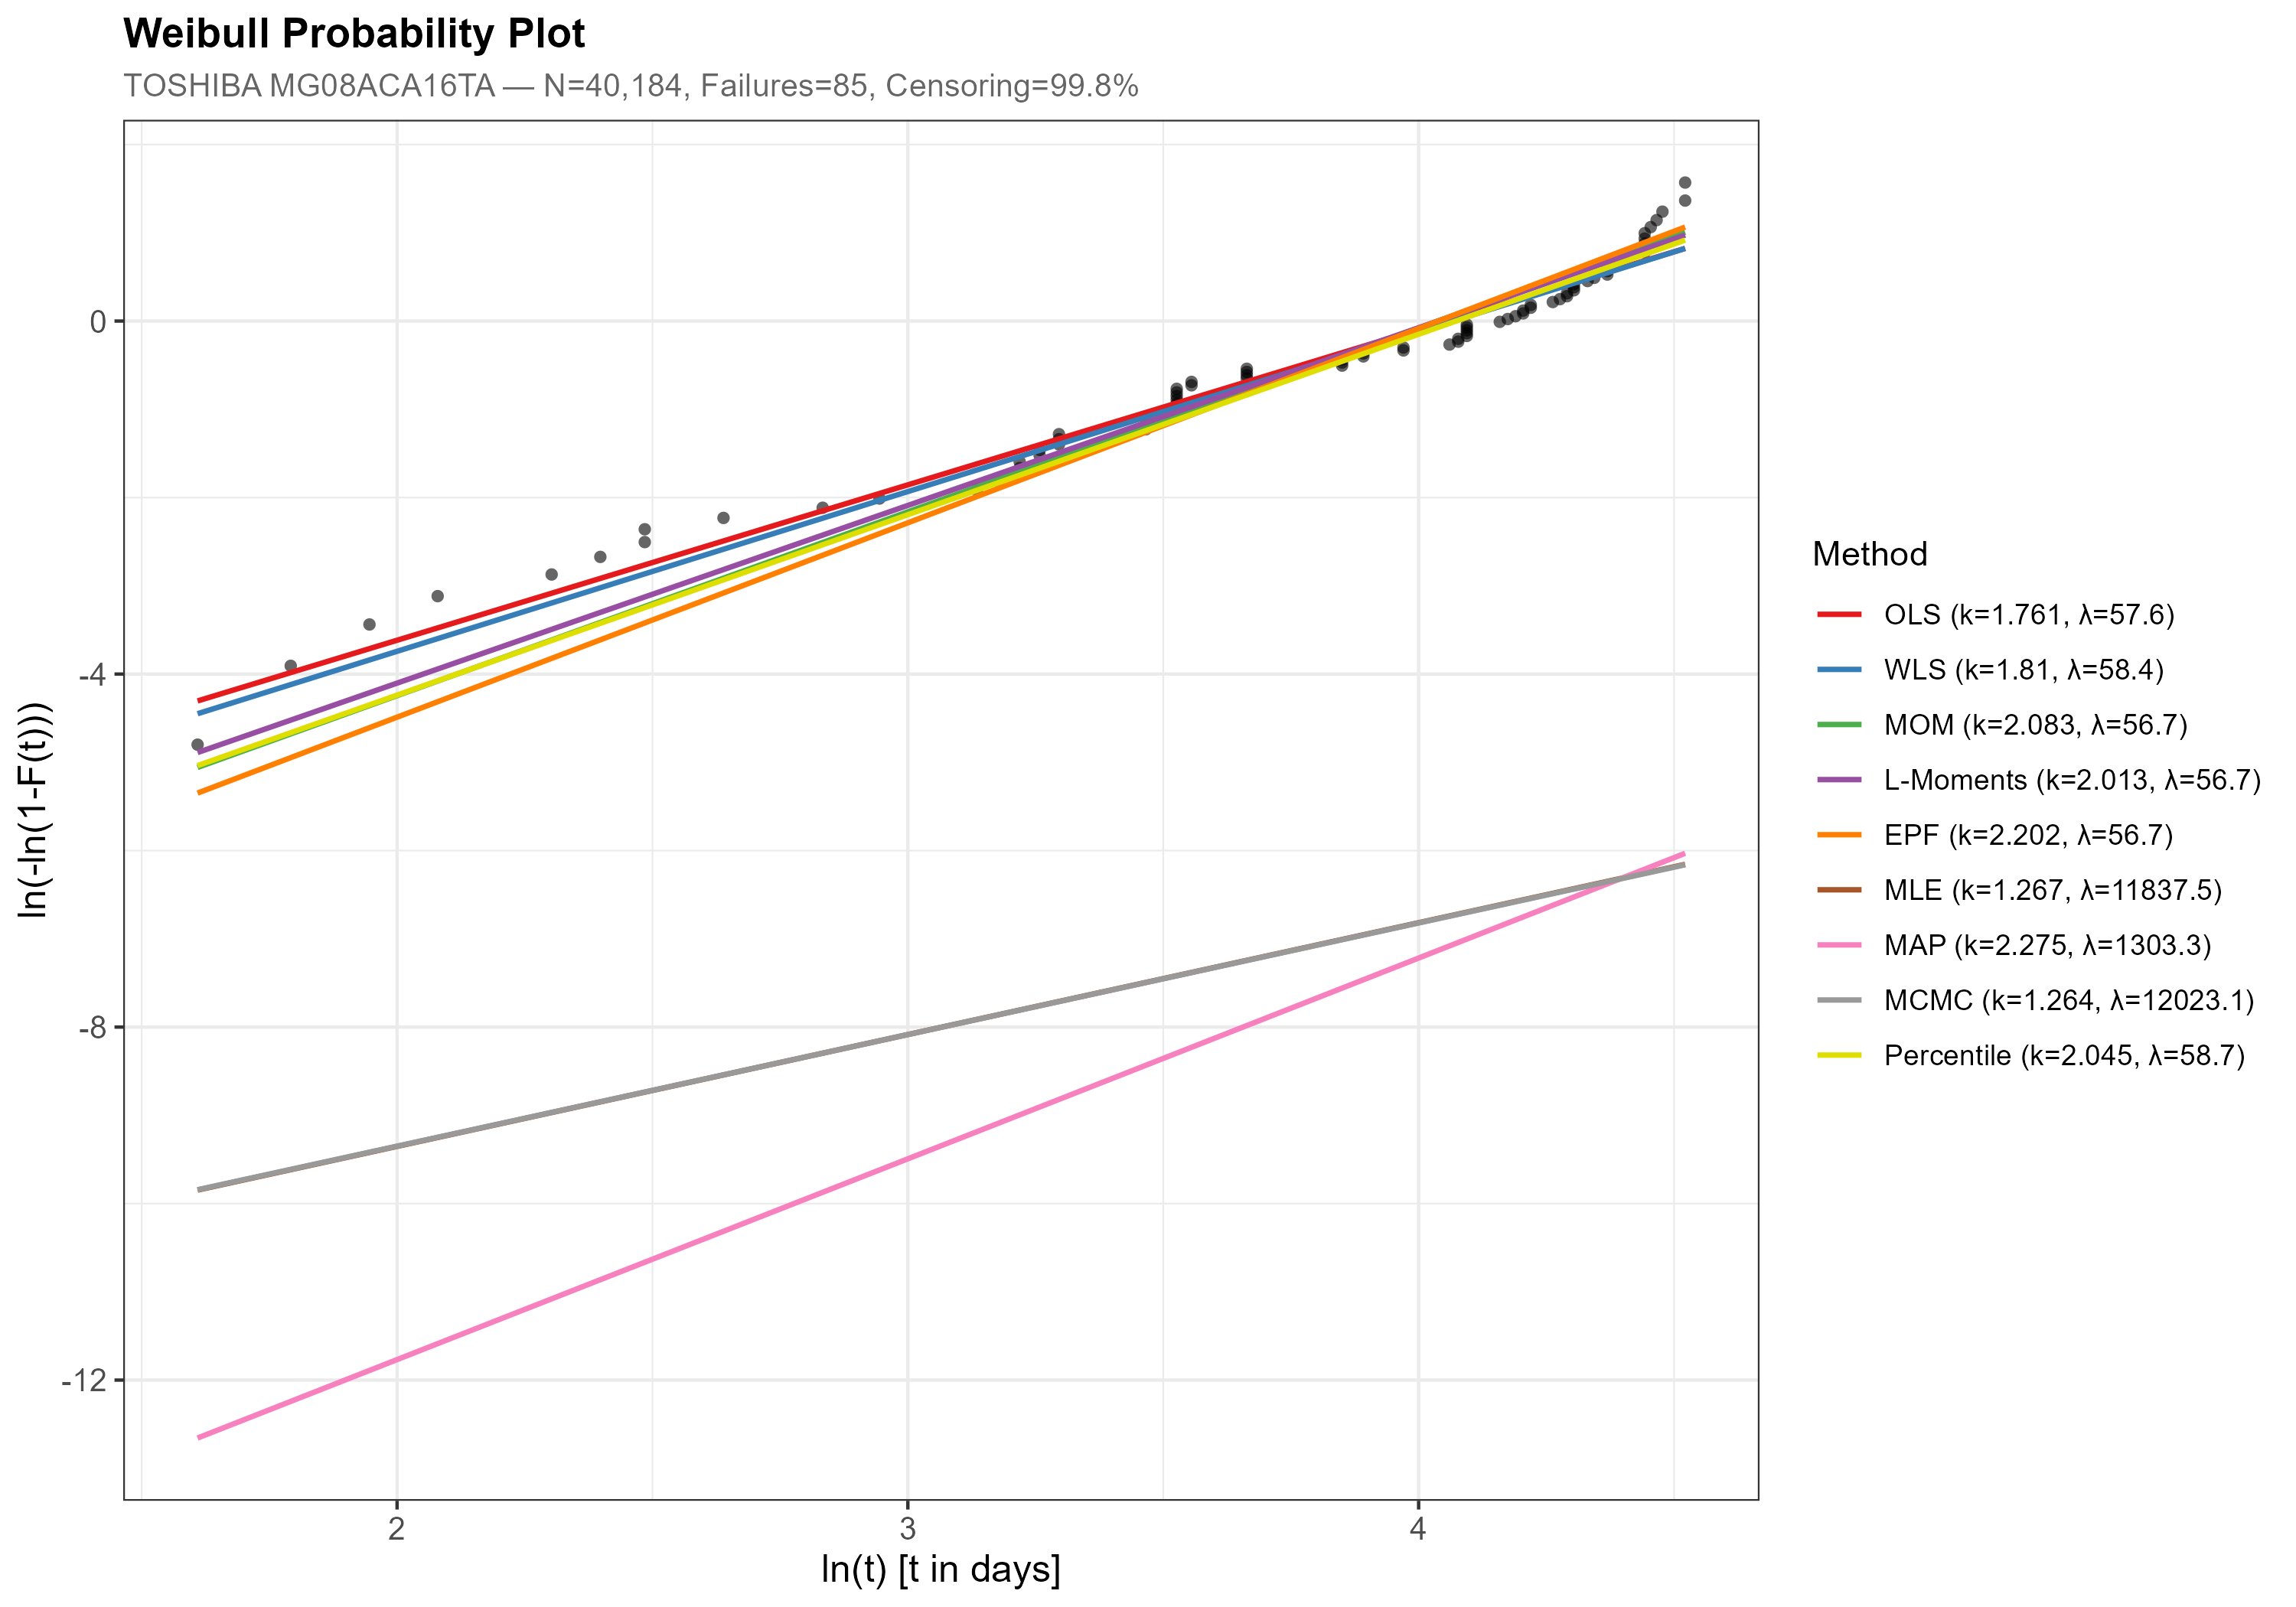
\includegraphics[width=0.95\linewidth]{results/plots/plot1_weibull_probability_TOSHIBA_MG08ACA16TA.png}
\caption{plot1 weibull probability — TOSHIBA MG08ACA16TA}
\end{figure}

\begin{figure}[H]
\centering
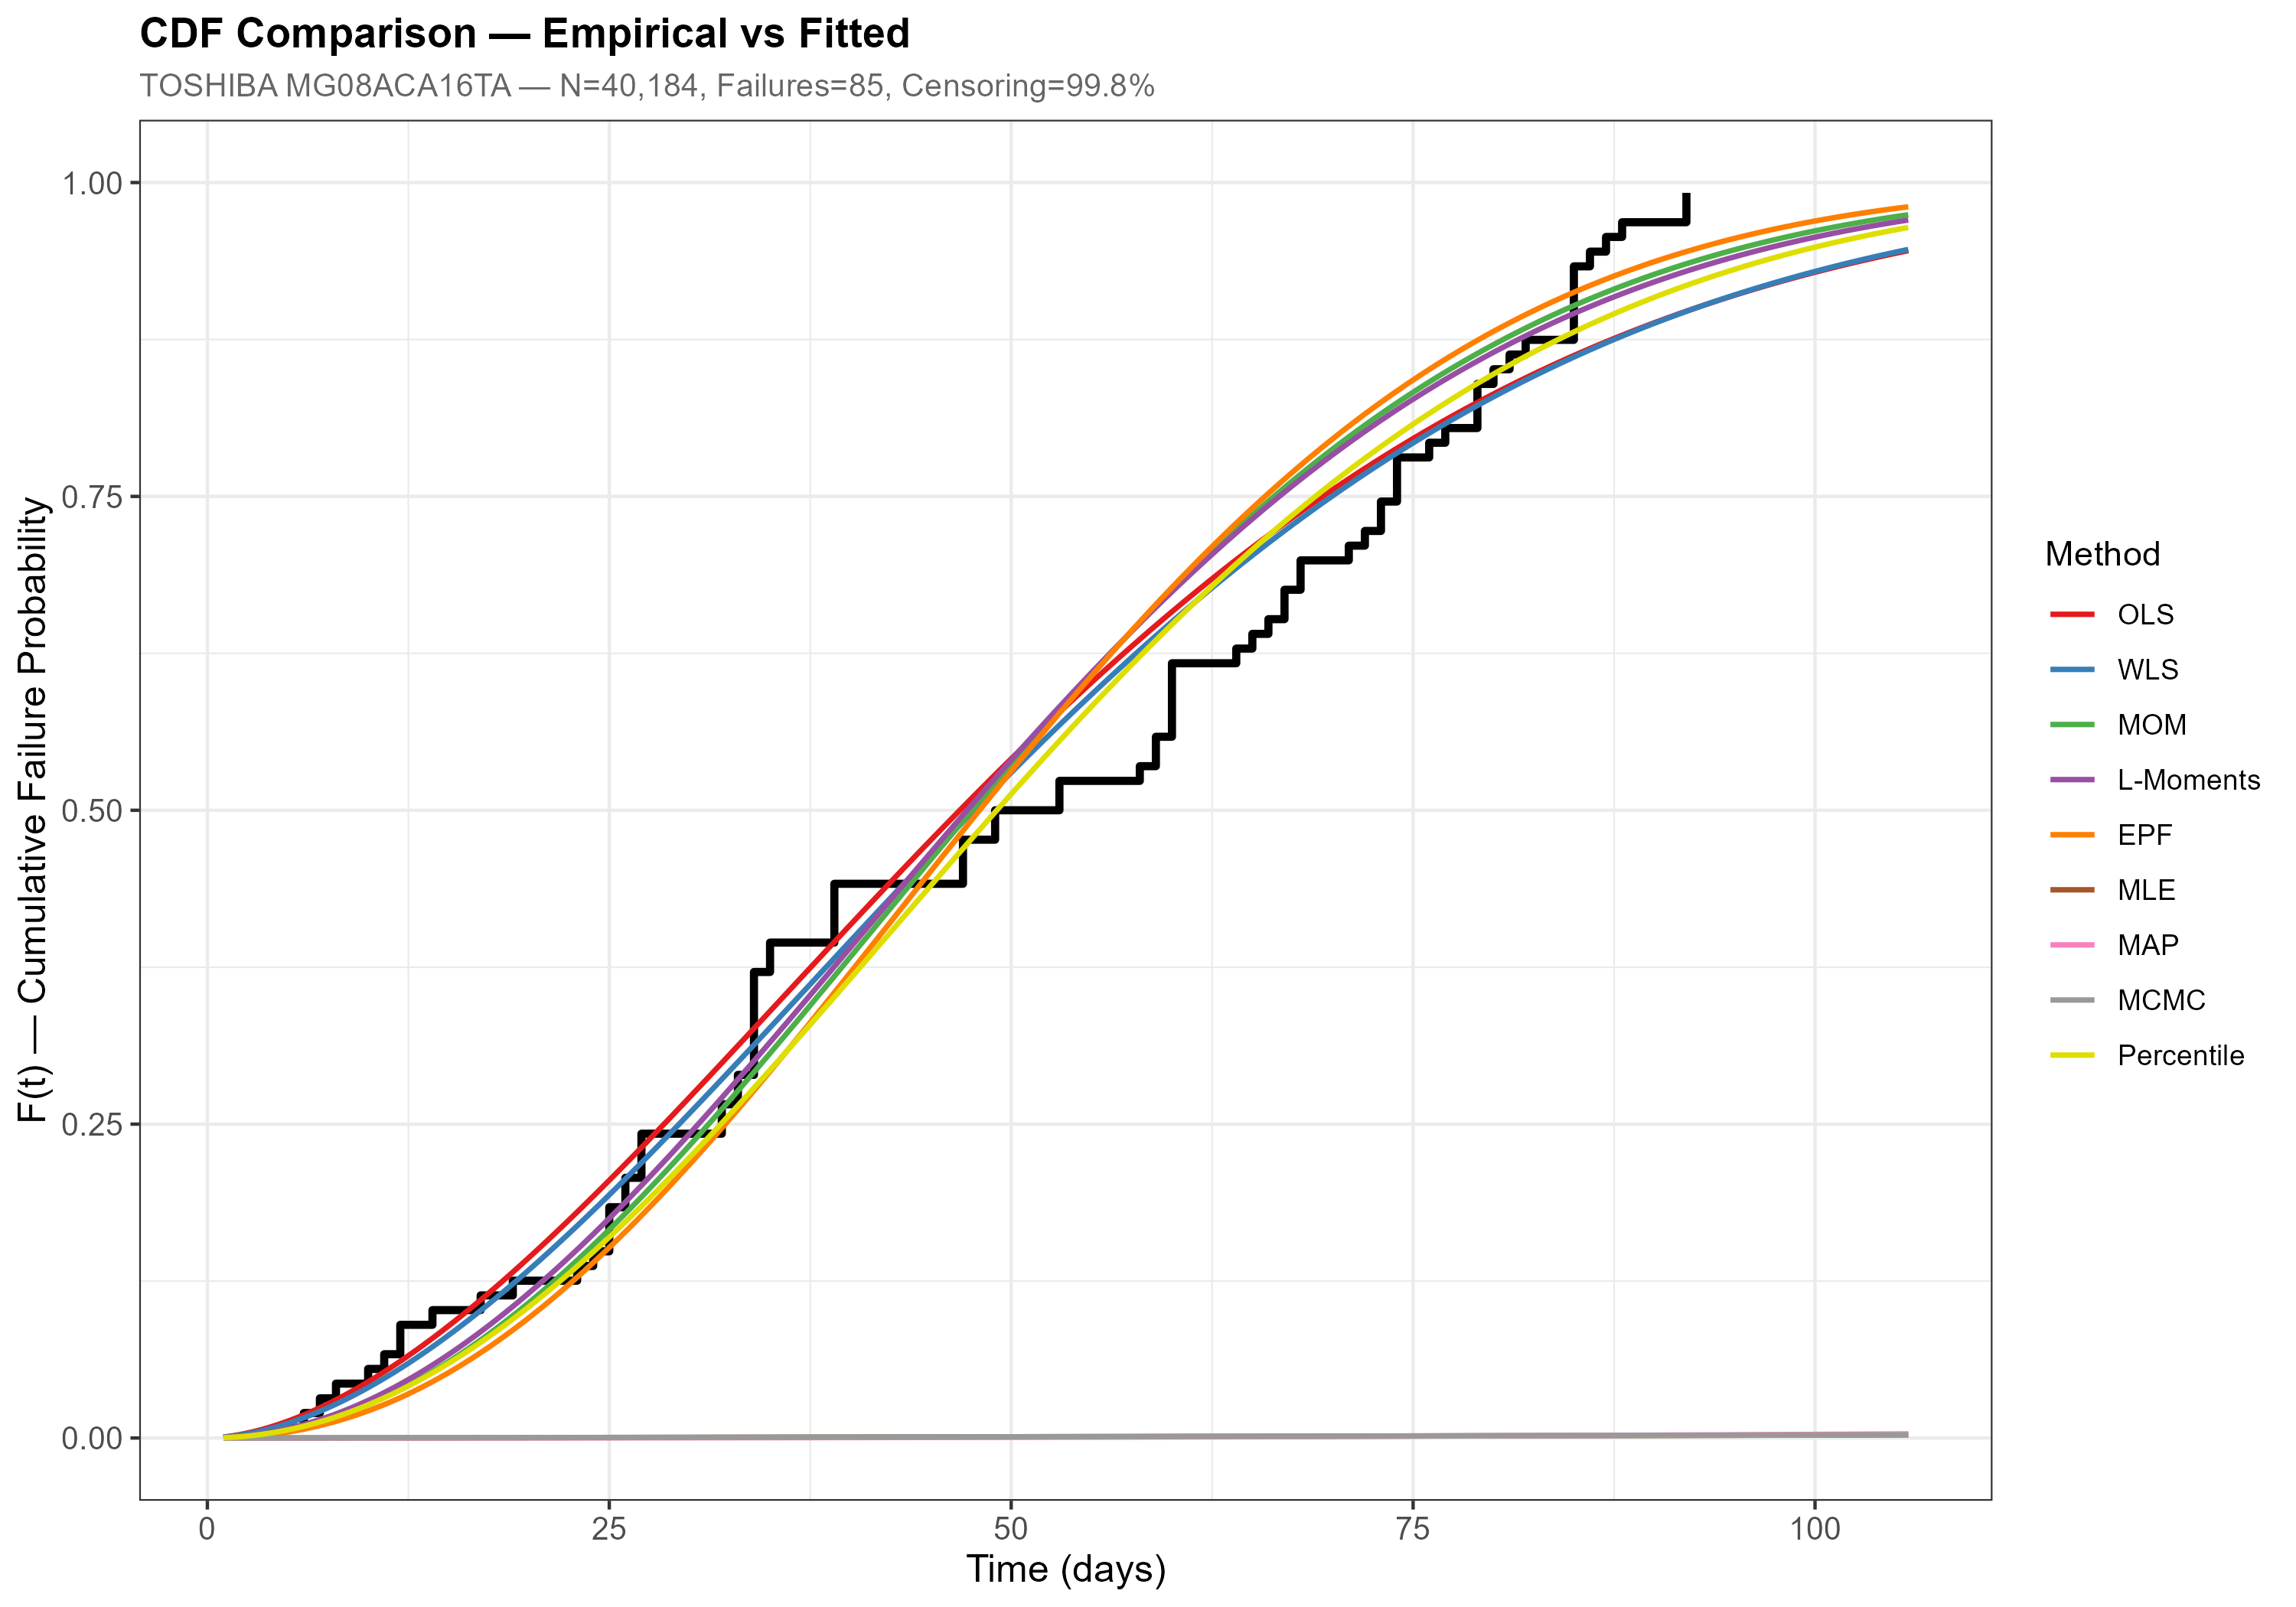
\includegraphics[width=0.95\linewidth]{results/plots/plot2_cdf_TOSHIBA_MG08ACA16TA.png}
\caption{plot2 cdf — TOSHIBA MG08ACA16TA}
\end{figure}

\begin{figure}[H]
\centering
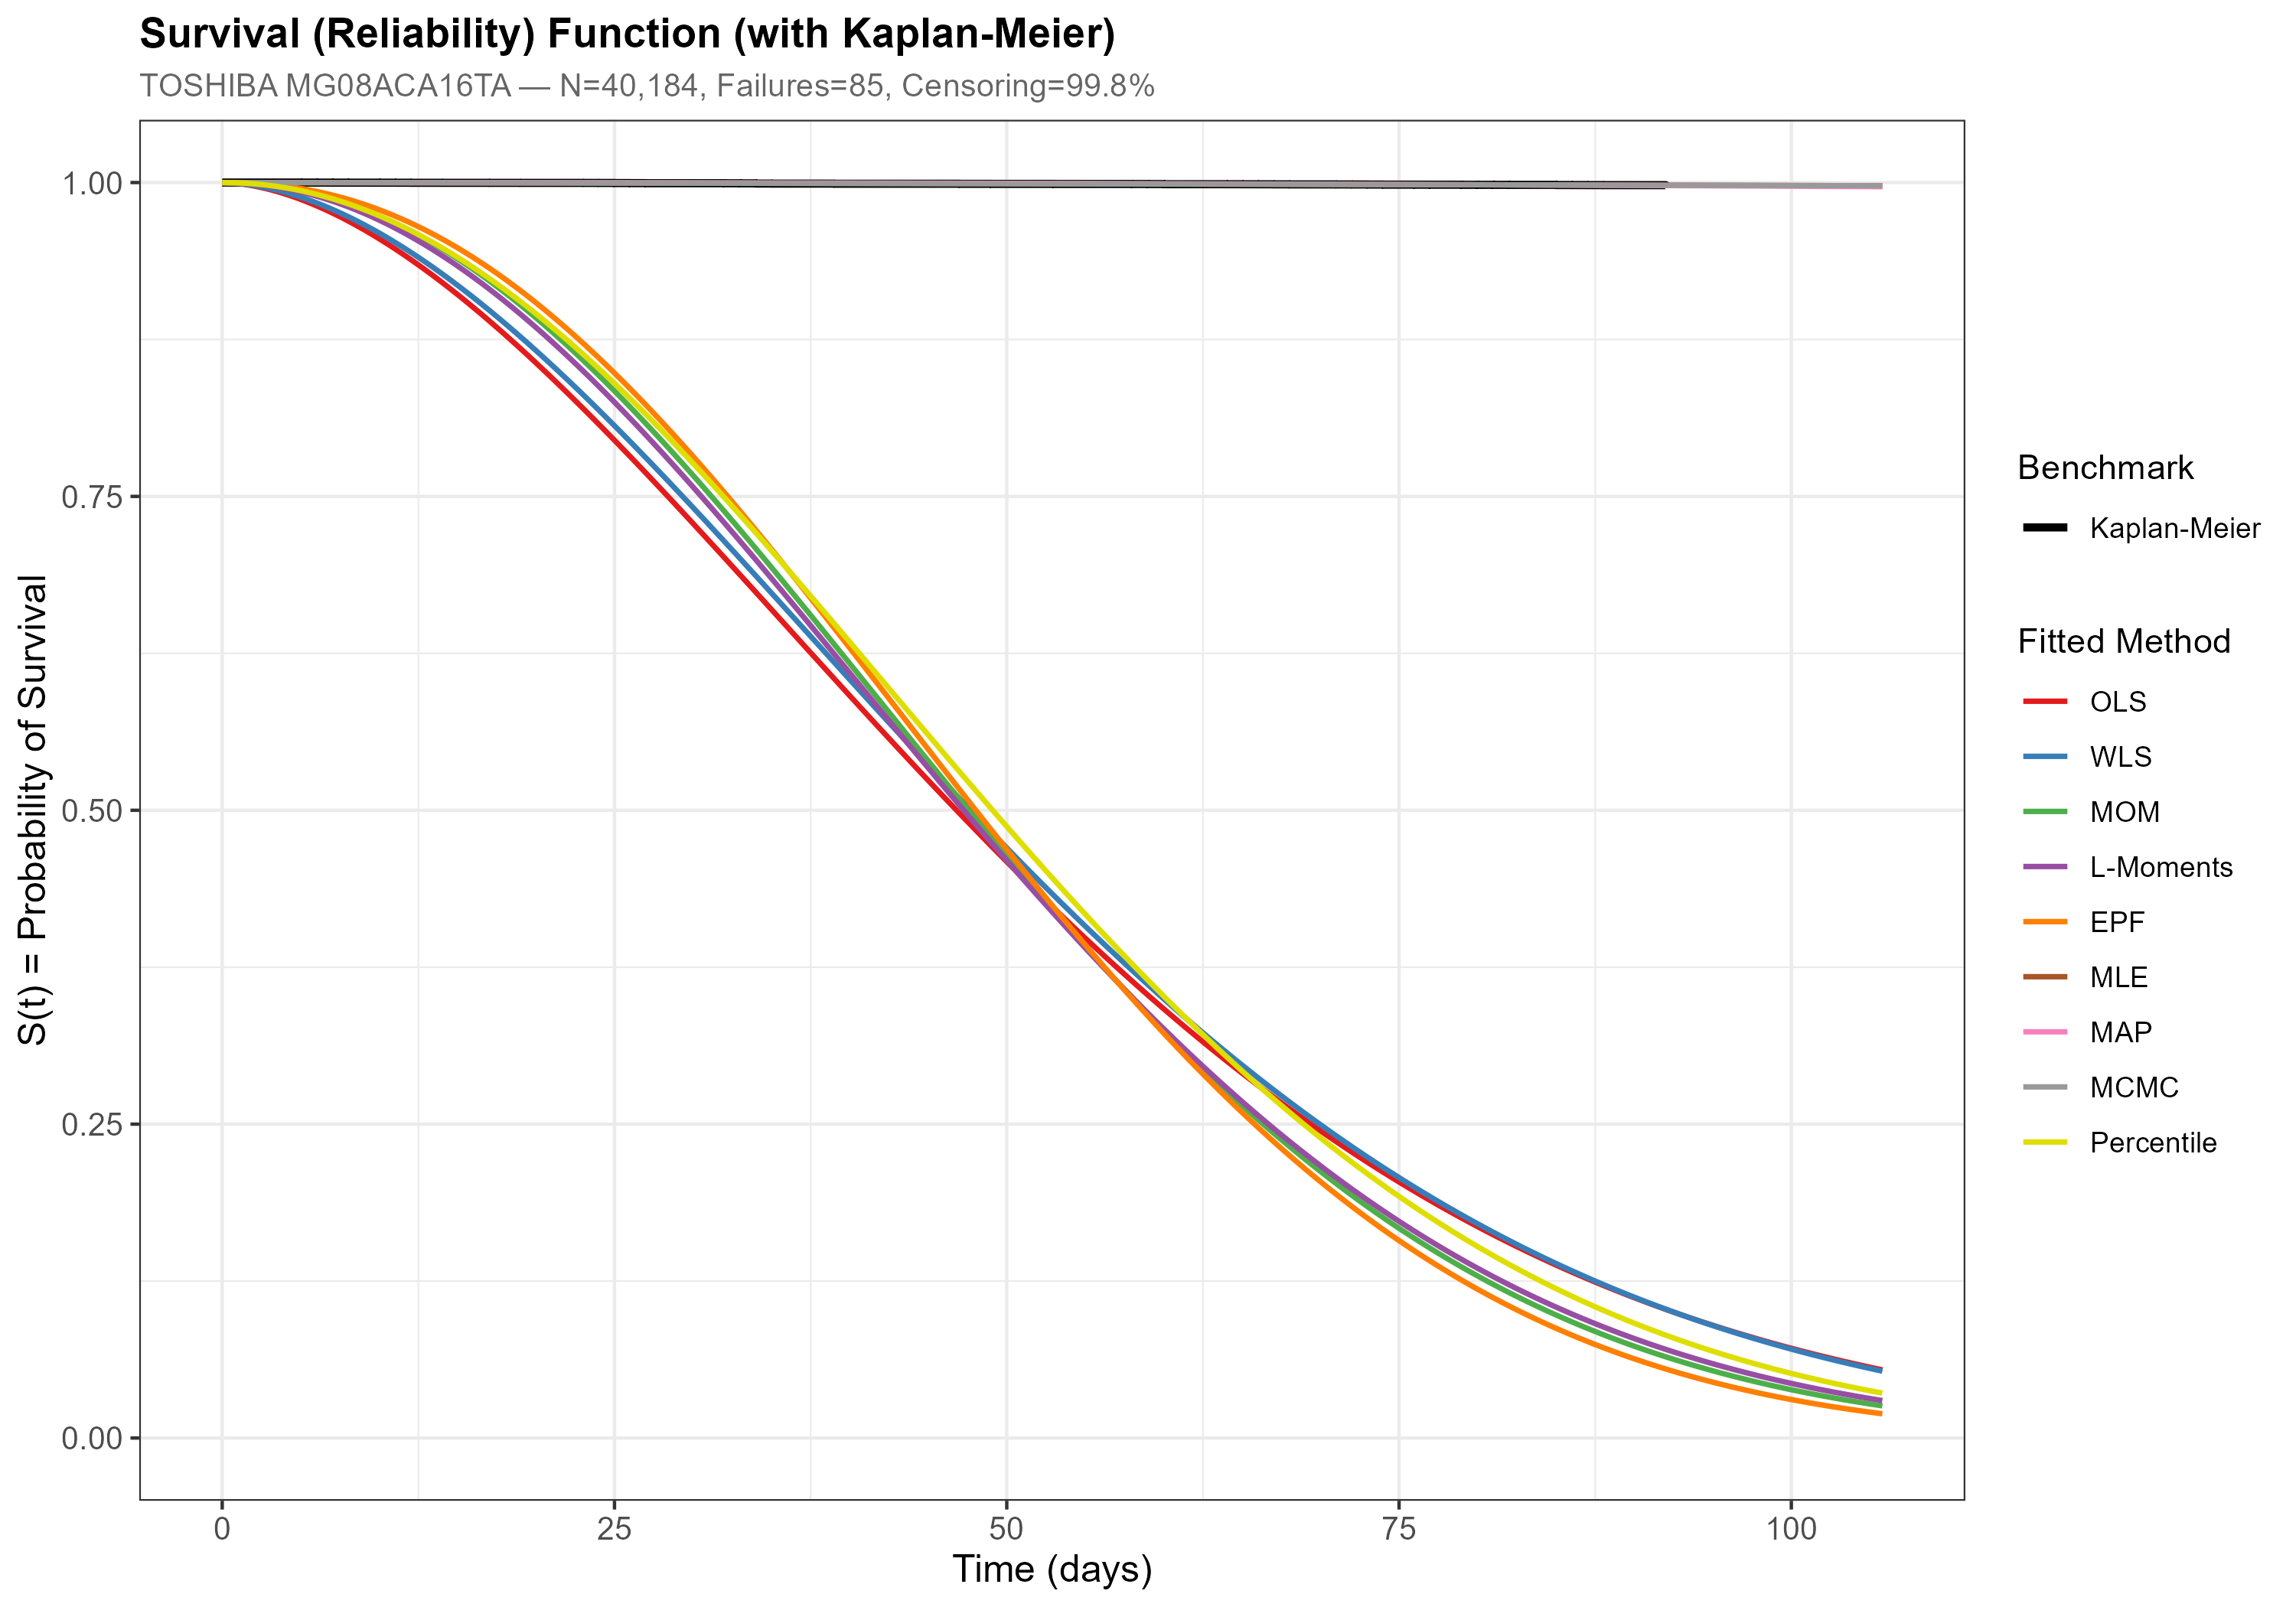
\includegraphics[width=0.95\linewidth]{results/plots/plot3_survival_TOSHIBA_MG08ACA16TA.png}
\caption{plot3 survival — TOSHIBA MG08ACA16TA}
\end{figure}

\begin{figure}[H]
\centering
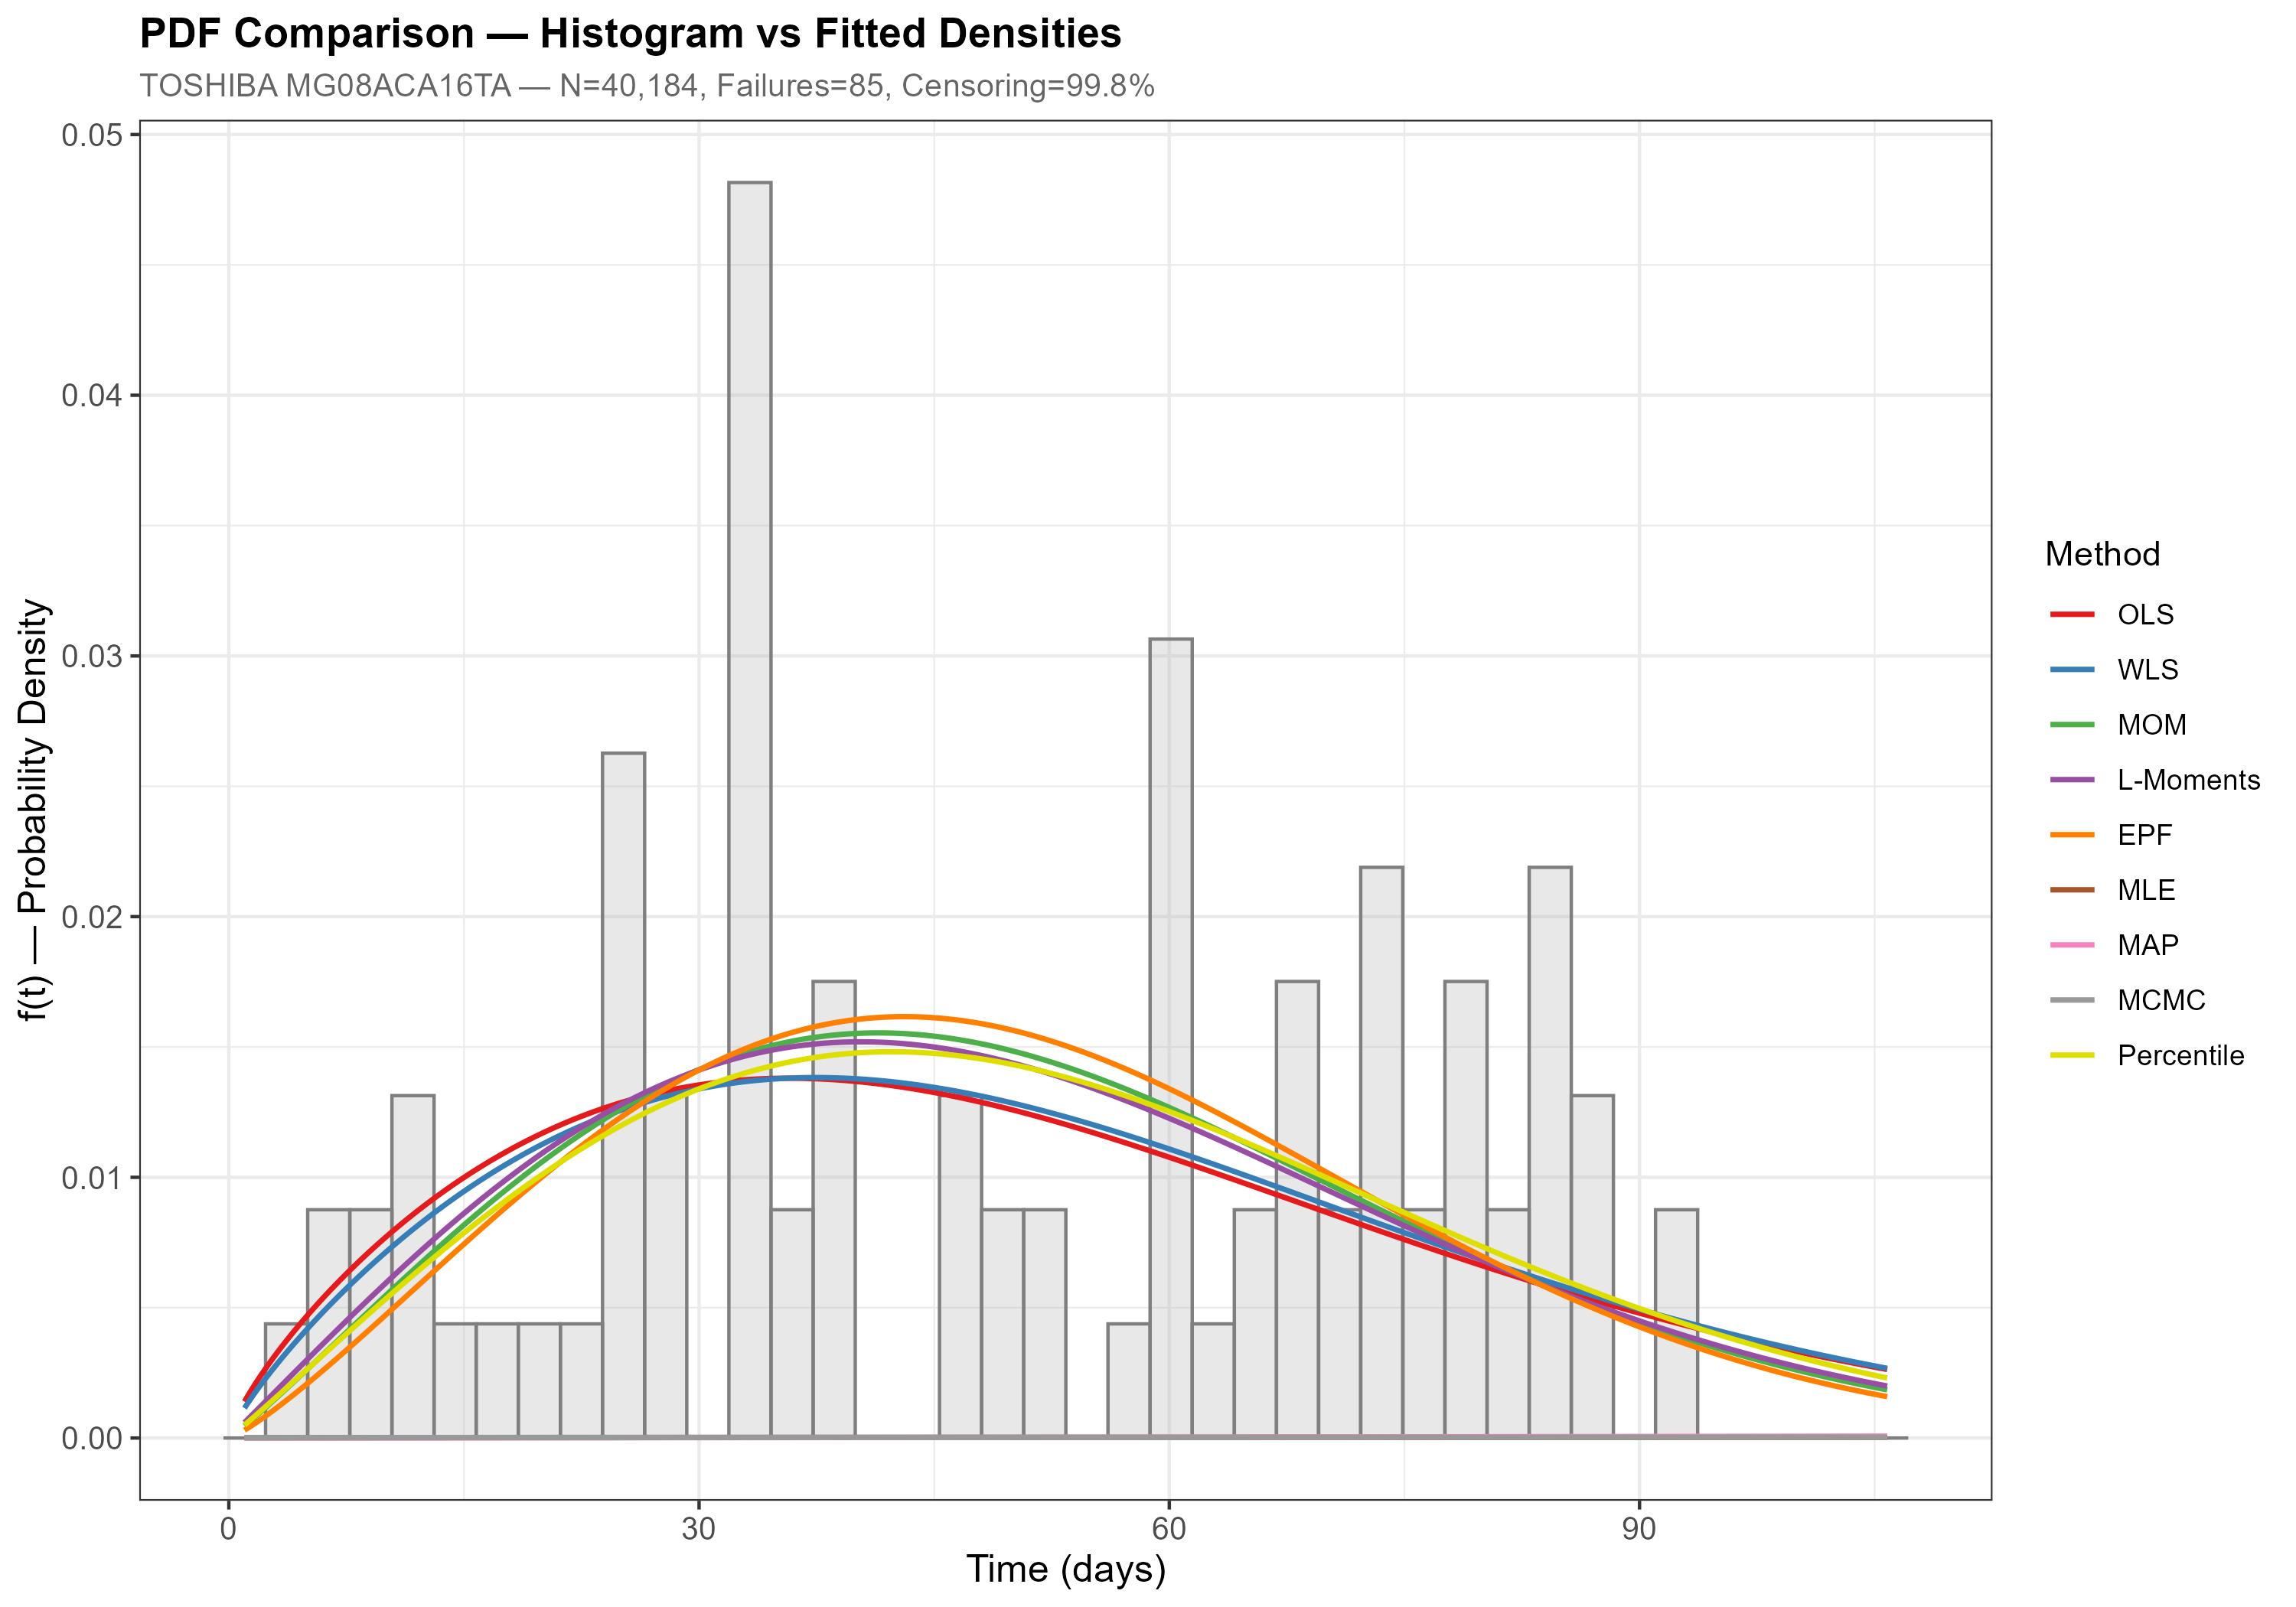
\includegraphics[width=0.95\linewidth]{results/plots/plot4_pdf_TOSHIBA_MG08ACA16TA.png}
\caption{plot4 pdf — TOSHIBA MG08ACA16TA}
\end{figure}

\begin{figure}[H]
\centering
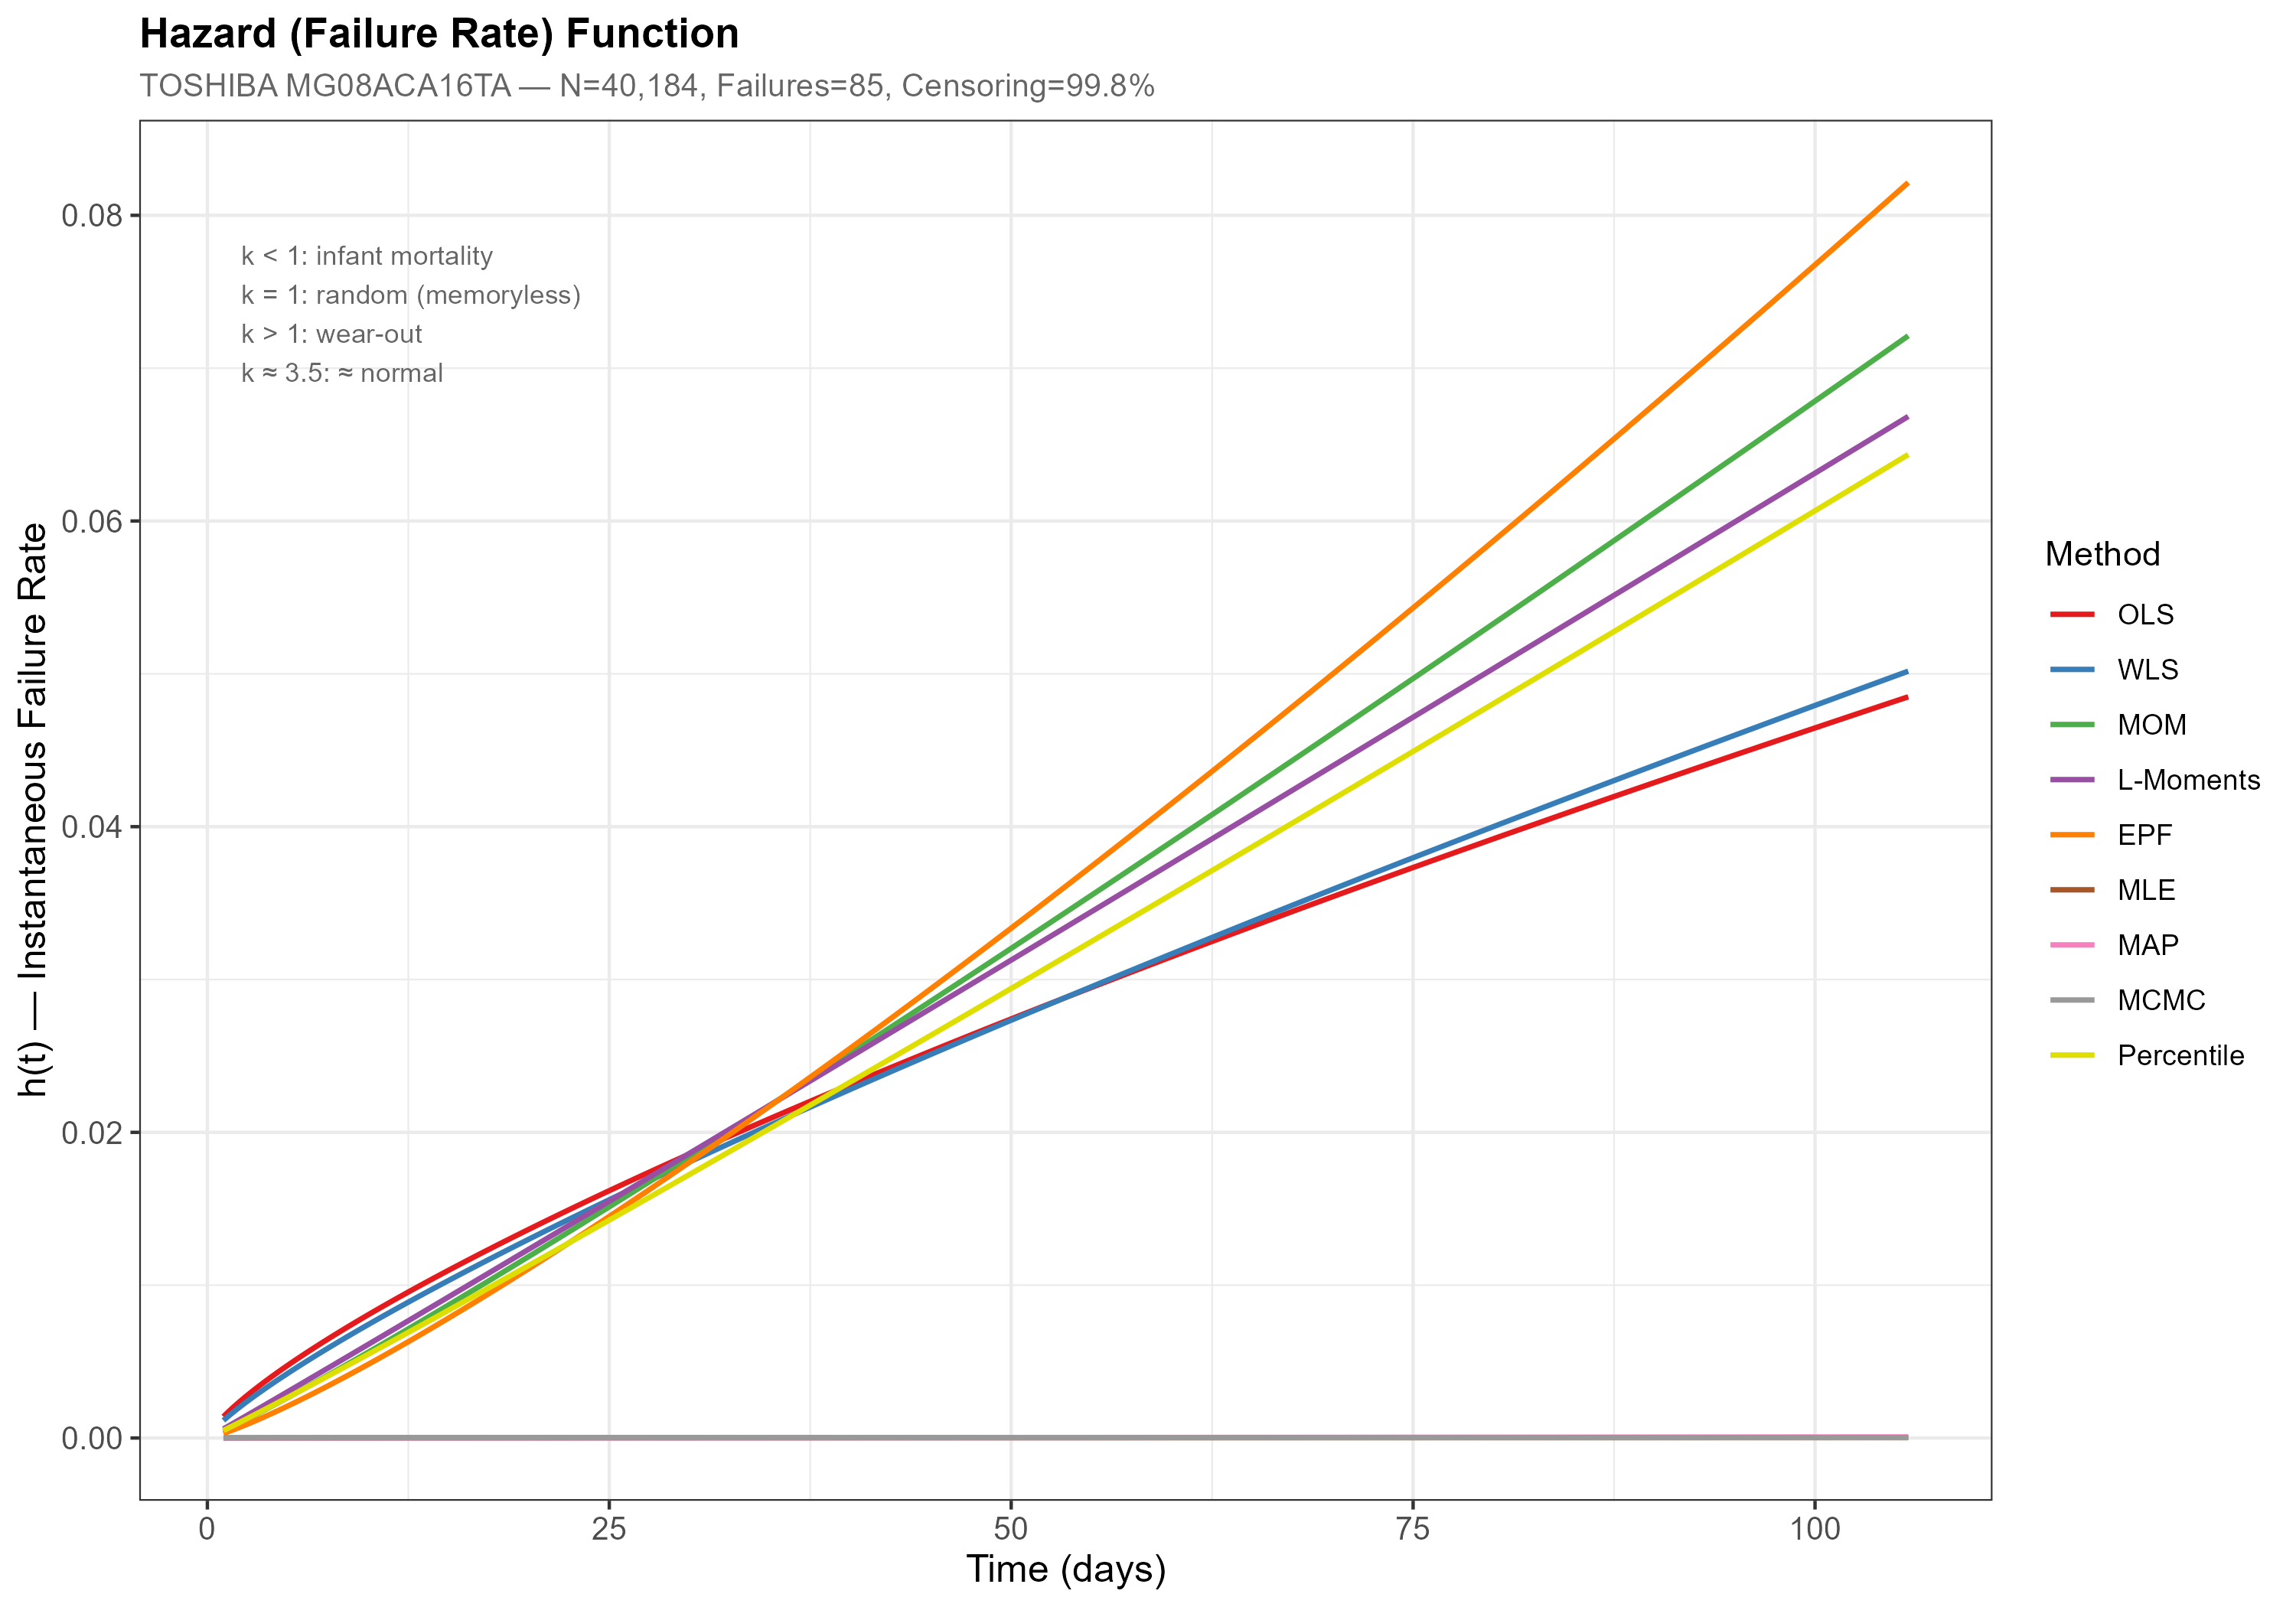
\includegraphics[width=0.95\linewidth]{results/plots/plot5_hazard_TOSHIBA_MG08ACA16TA.png}
\caption{plot5 hazard — TOSHIBA MG08ACA16TA}
\end{figure}

\begin{figure}[H]
\centering
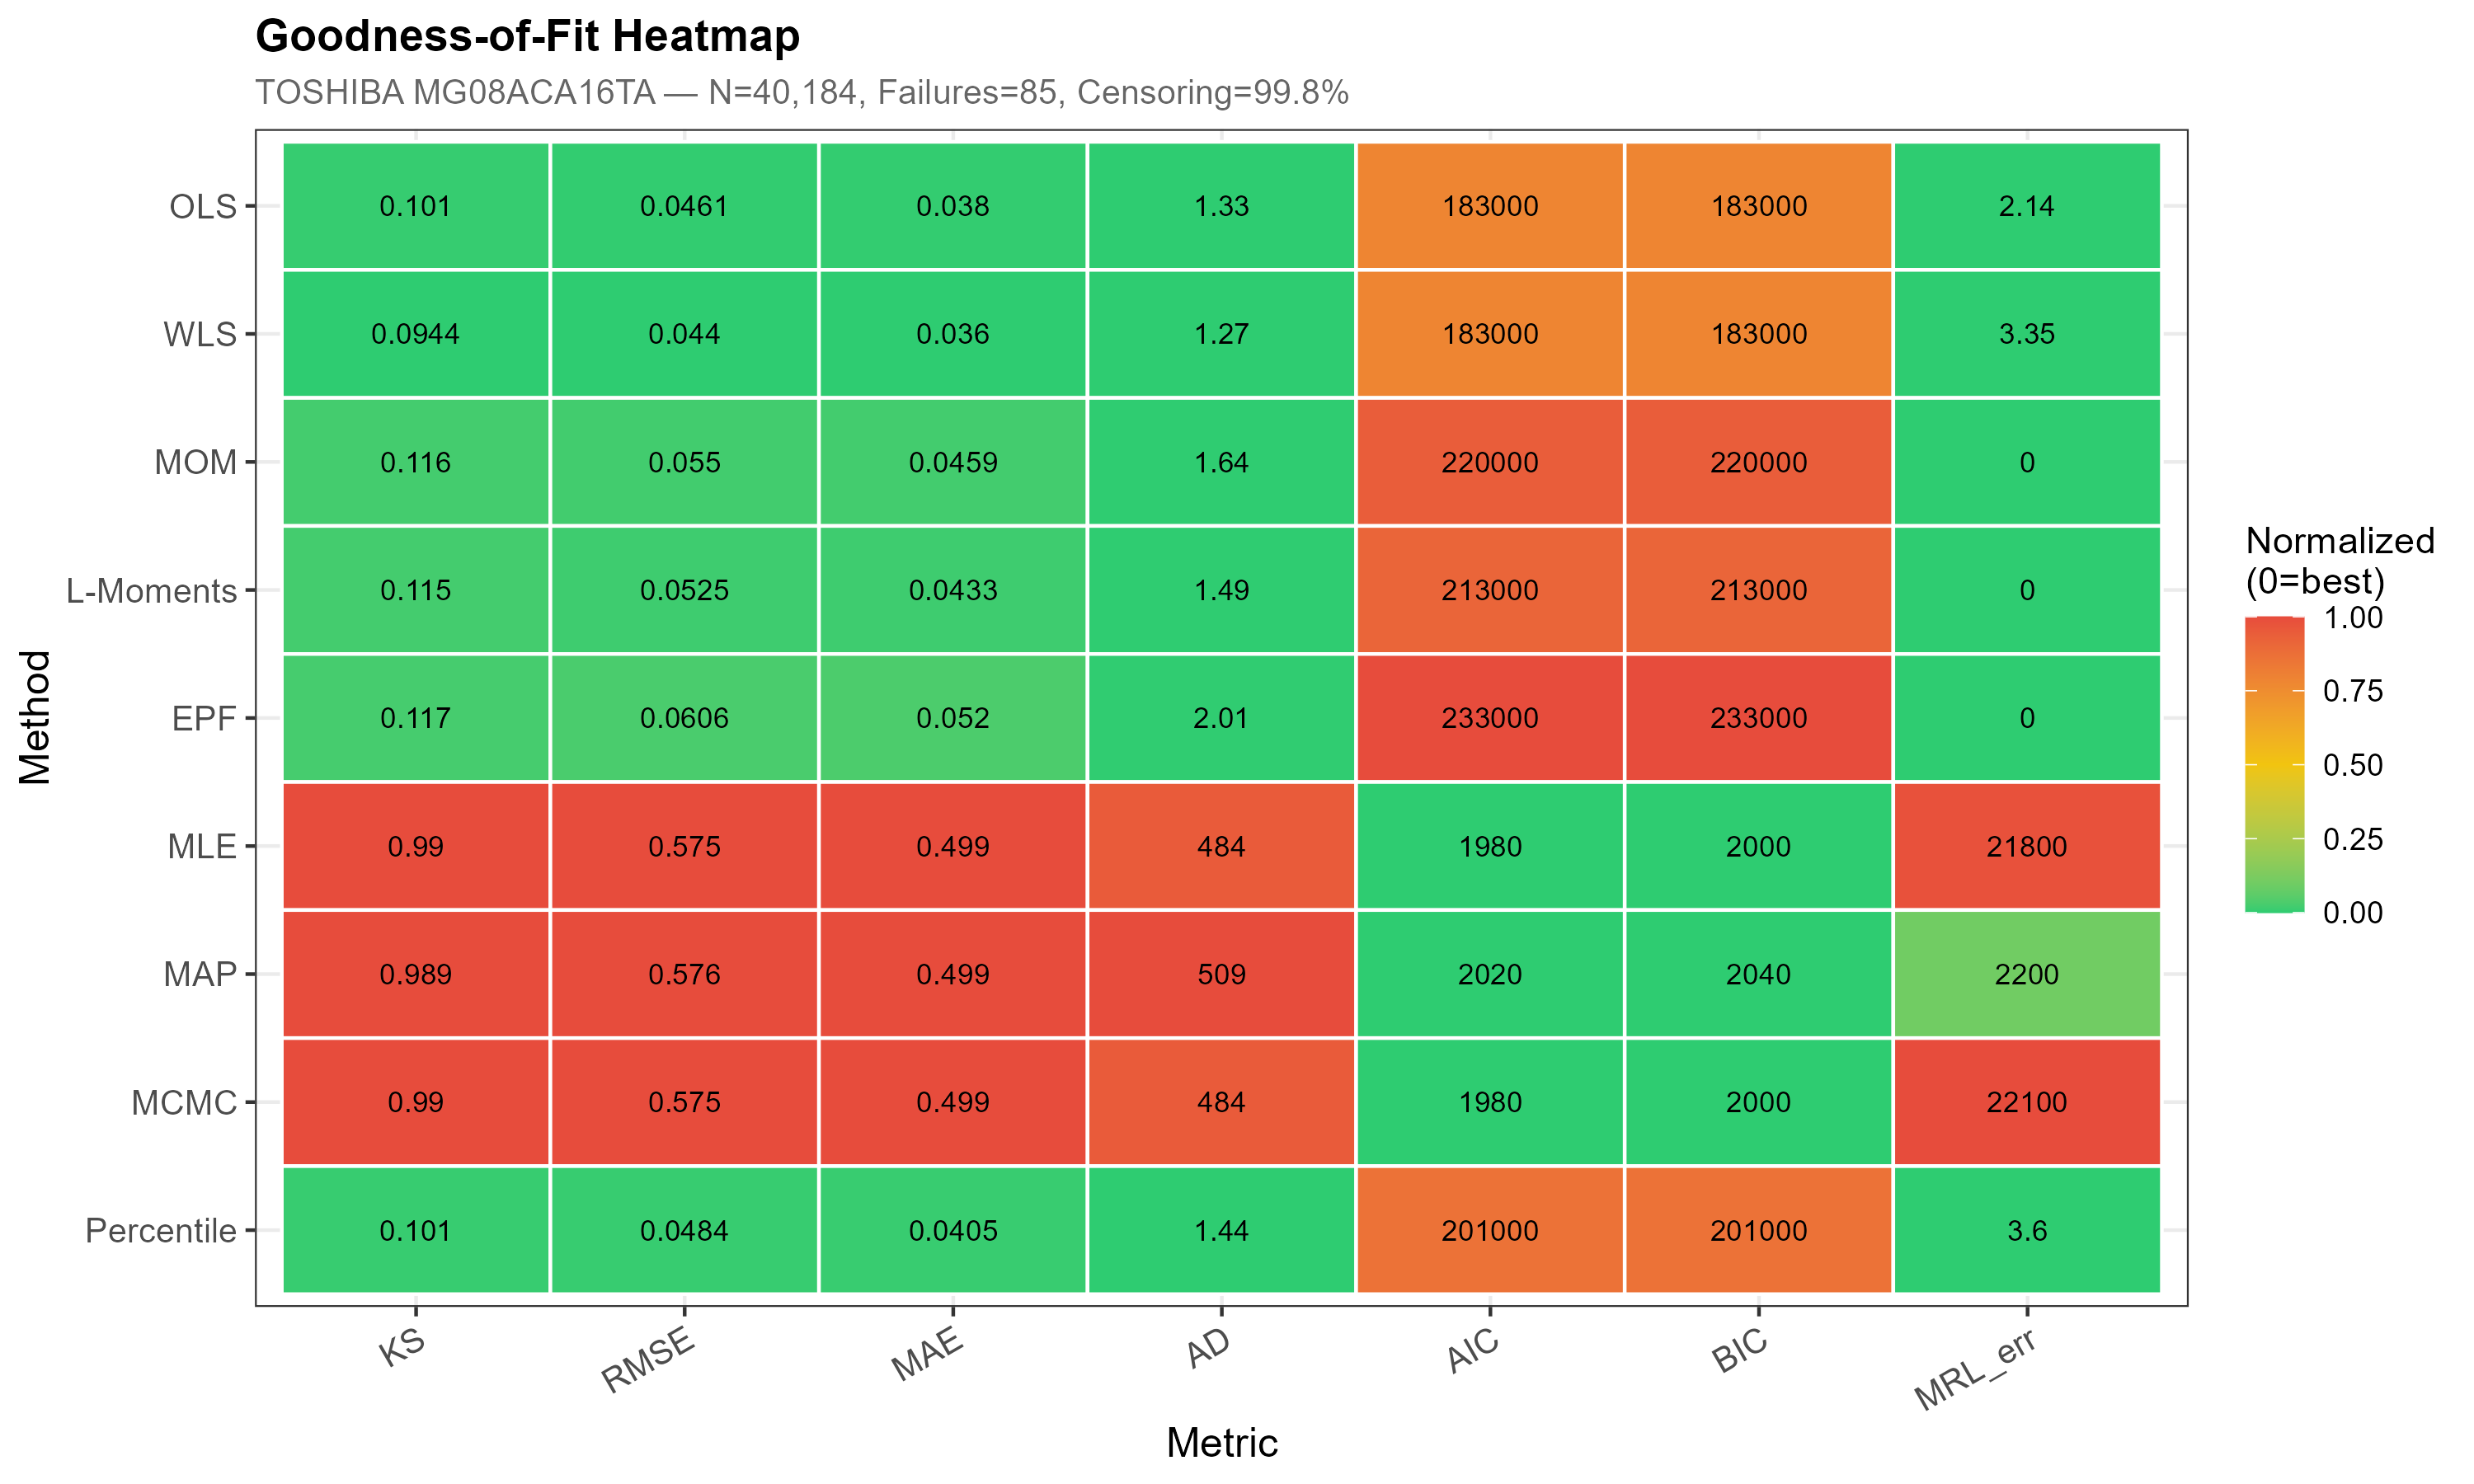
\includegraphics[width=0.95\linewidth]{results/plots/plot6_gof_heatmap_TOSHIBA_MG08ACA16TA.png}
\caption{plot6 gof heatmap — TOSHIBA MG08ACA16TA}
\end{figure}

\begin{figure}[H]
\centering
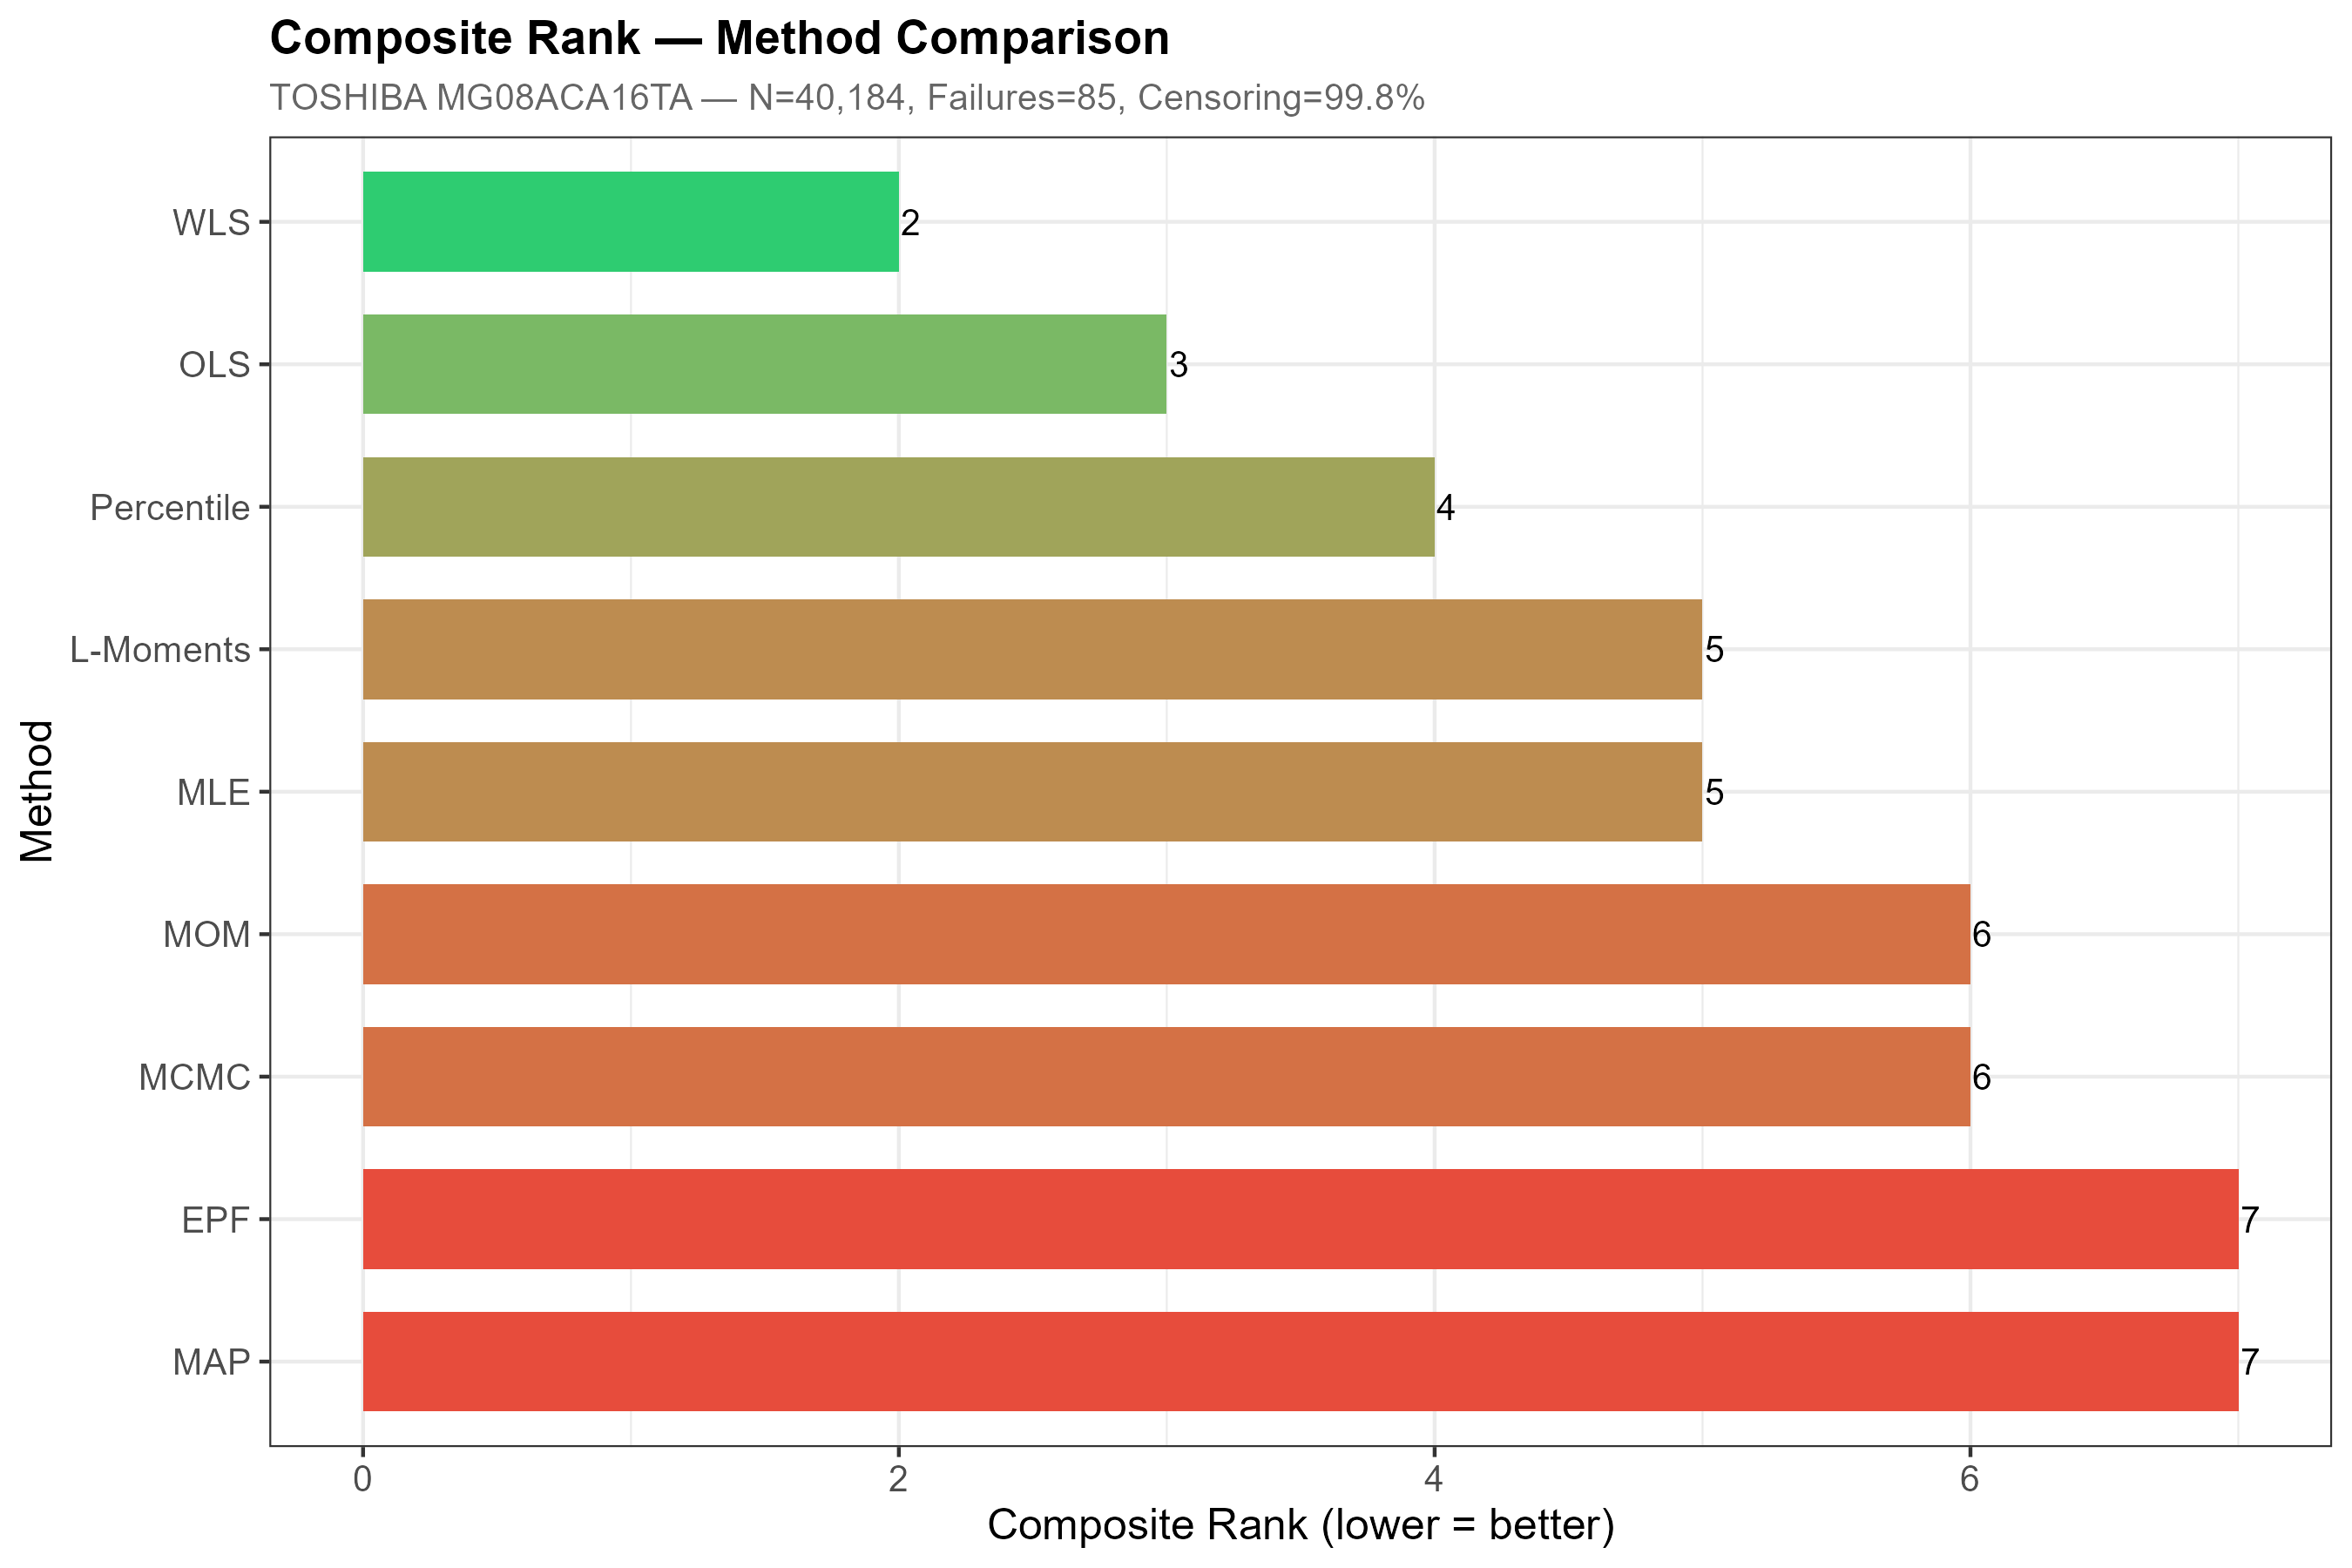
\includegraphics[width=0.95\linewidth]{results/plots/plot7_composite_rank_TOSHIBA_MG08ACA16TA.png}
\caption{plot7 composite rank — TOSHIBA MG08ACA16TA}
\end{figure}

\begin{figure}[H]
\centering
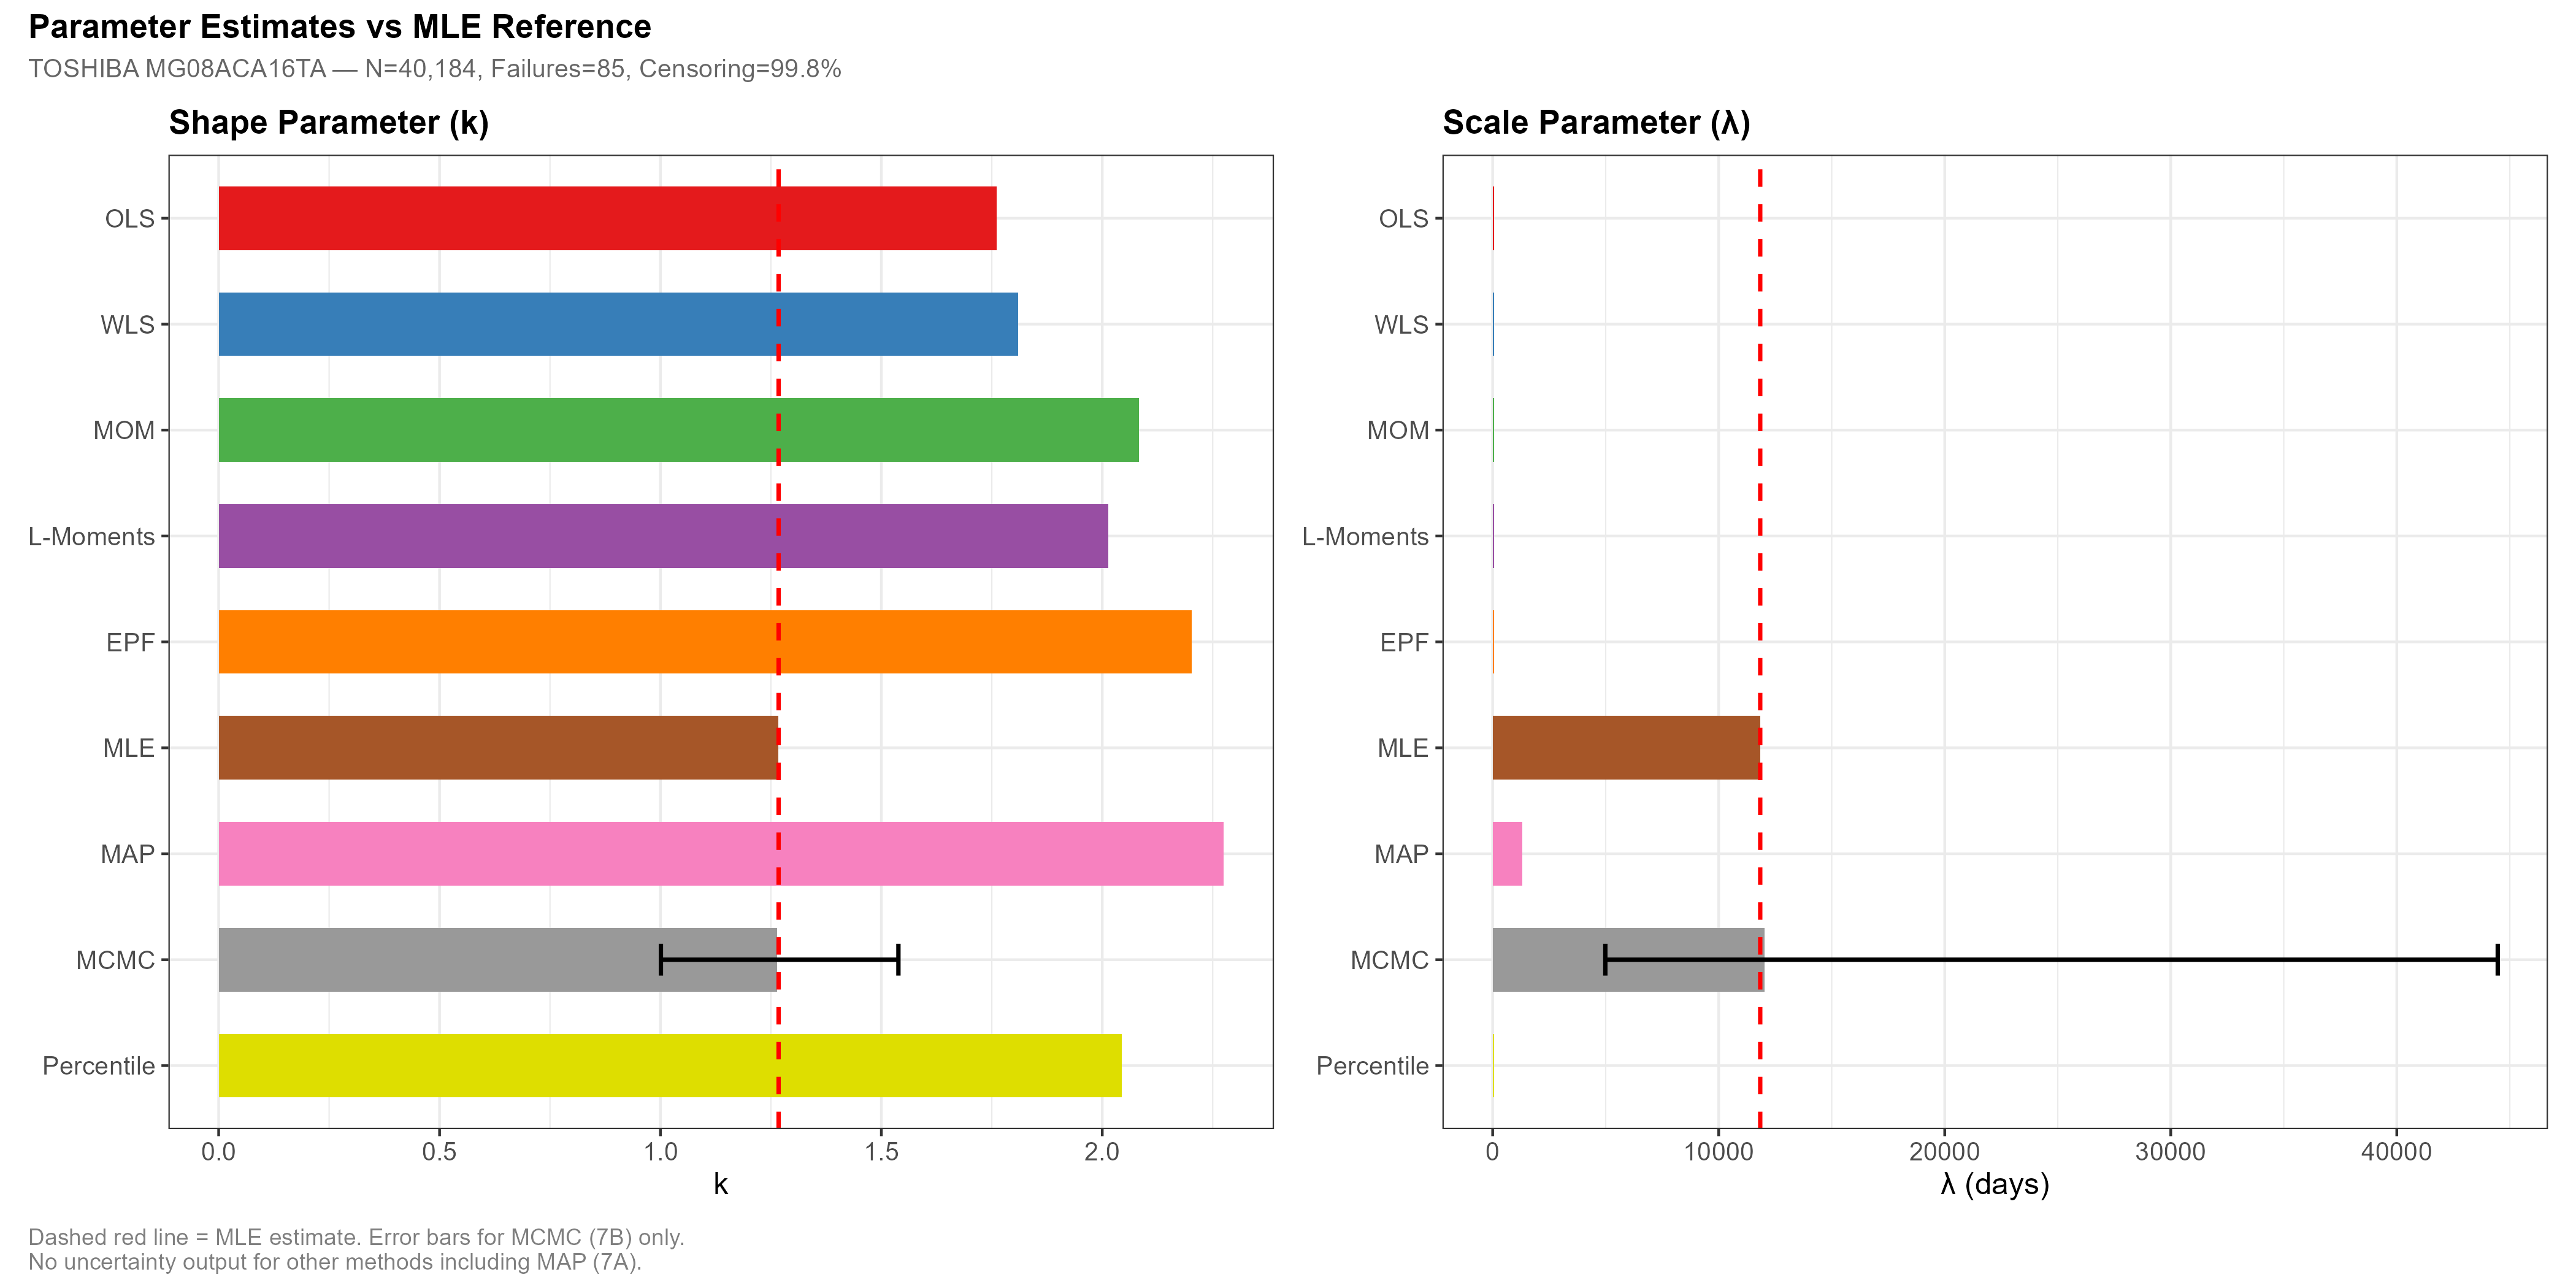
\includegraphics[width=0.95\linewidth]{results/plots/plot8_parameters_TOSHIBA_MG08ACA16TA.png}
\caption{plot8 parameters — TOSHIBA MG08ACA16TA}
\end{figure}

\subsection{WDC WUH722222ALE6L4}\label{wdc-wuh722222ale6l4}

\begin{figure}[H]
\centering
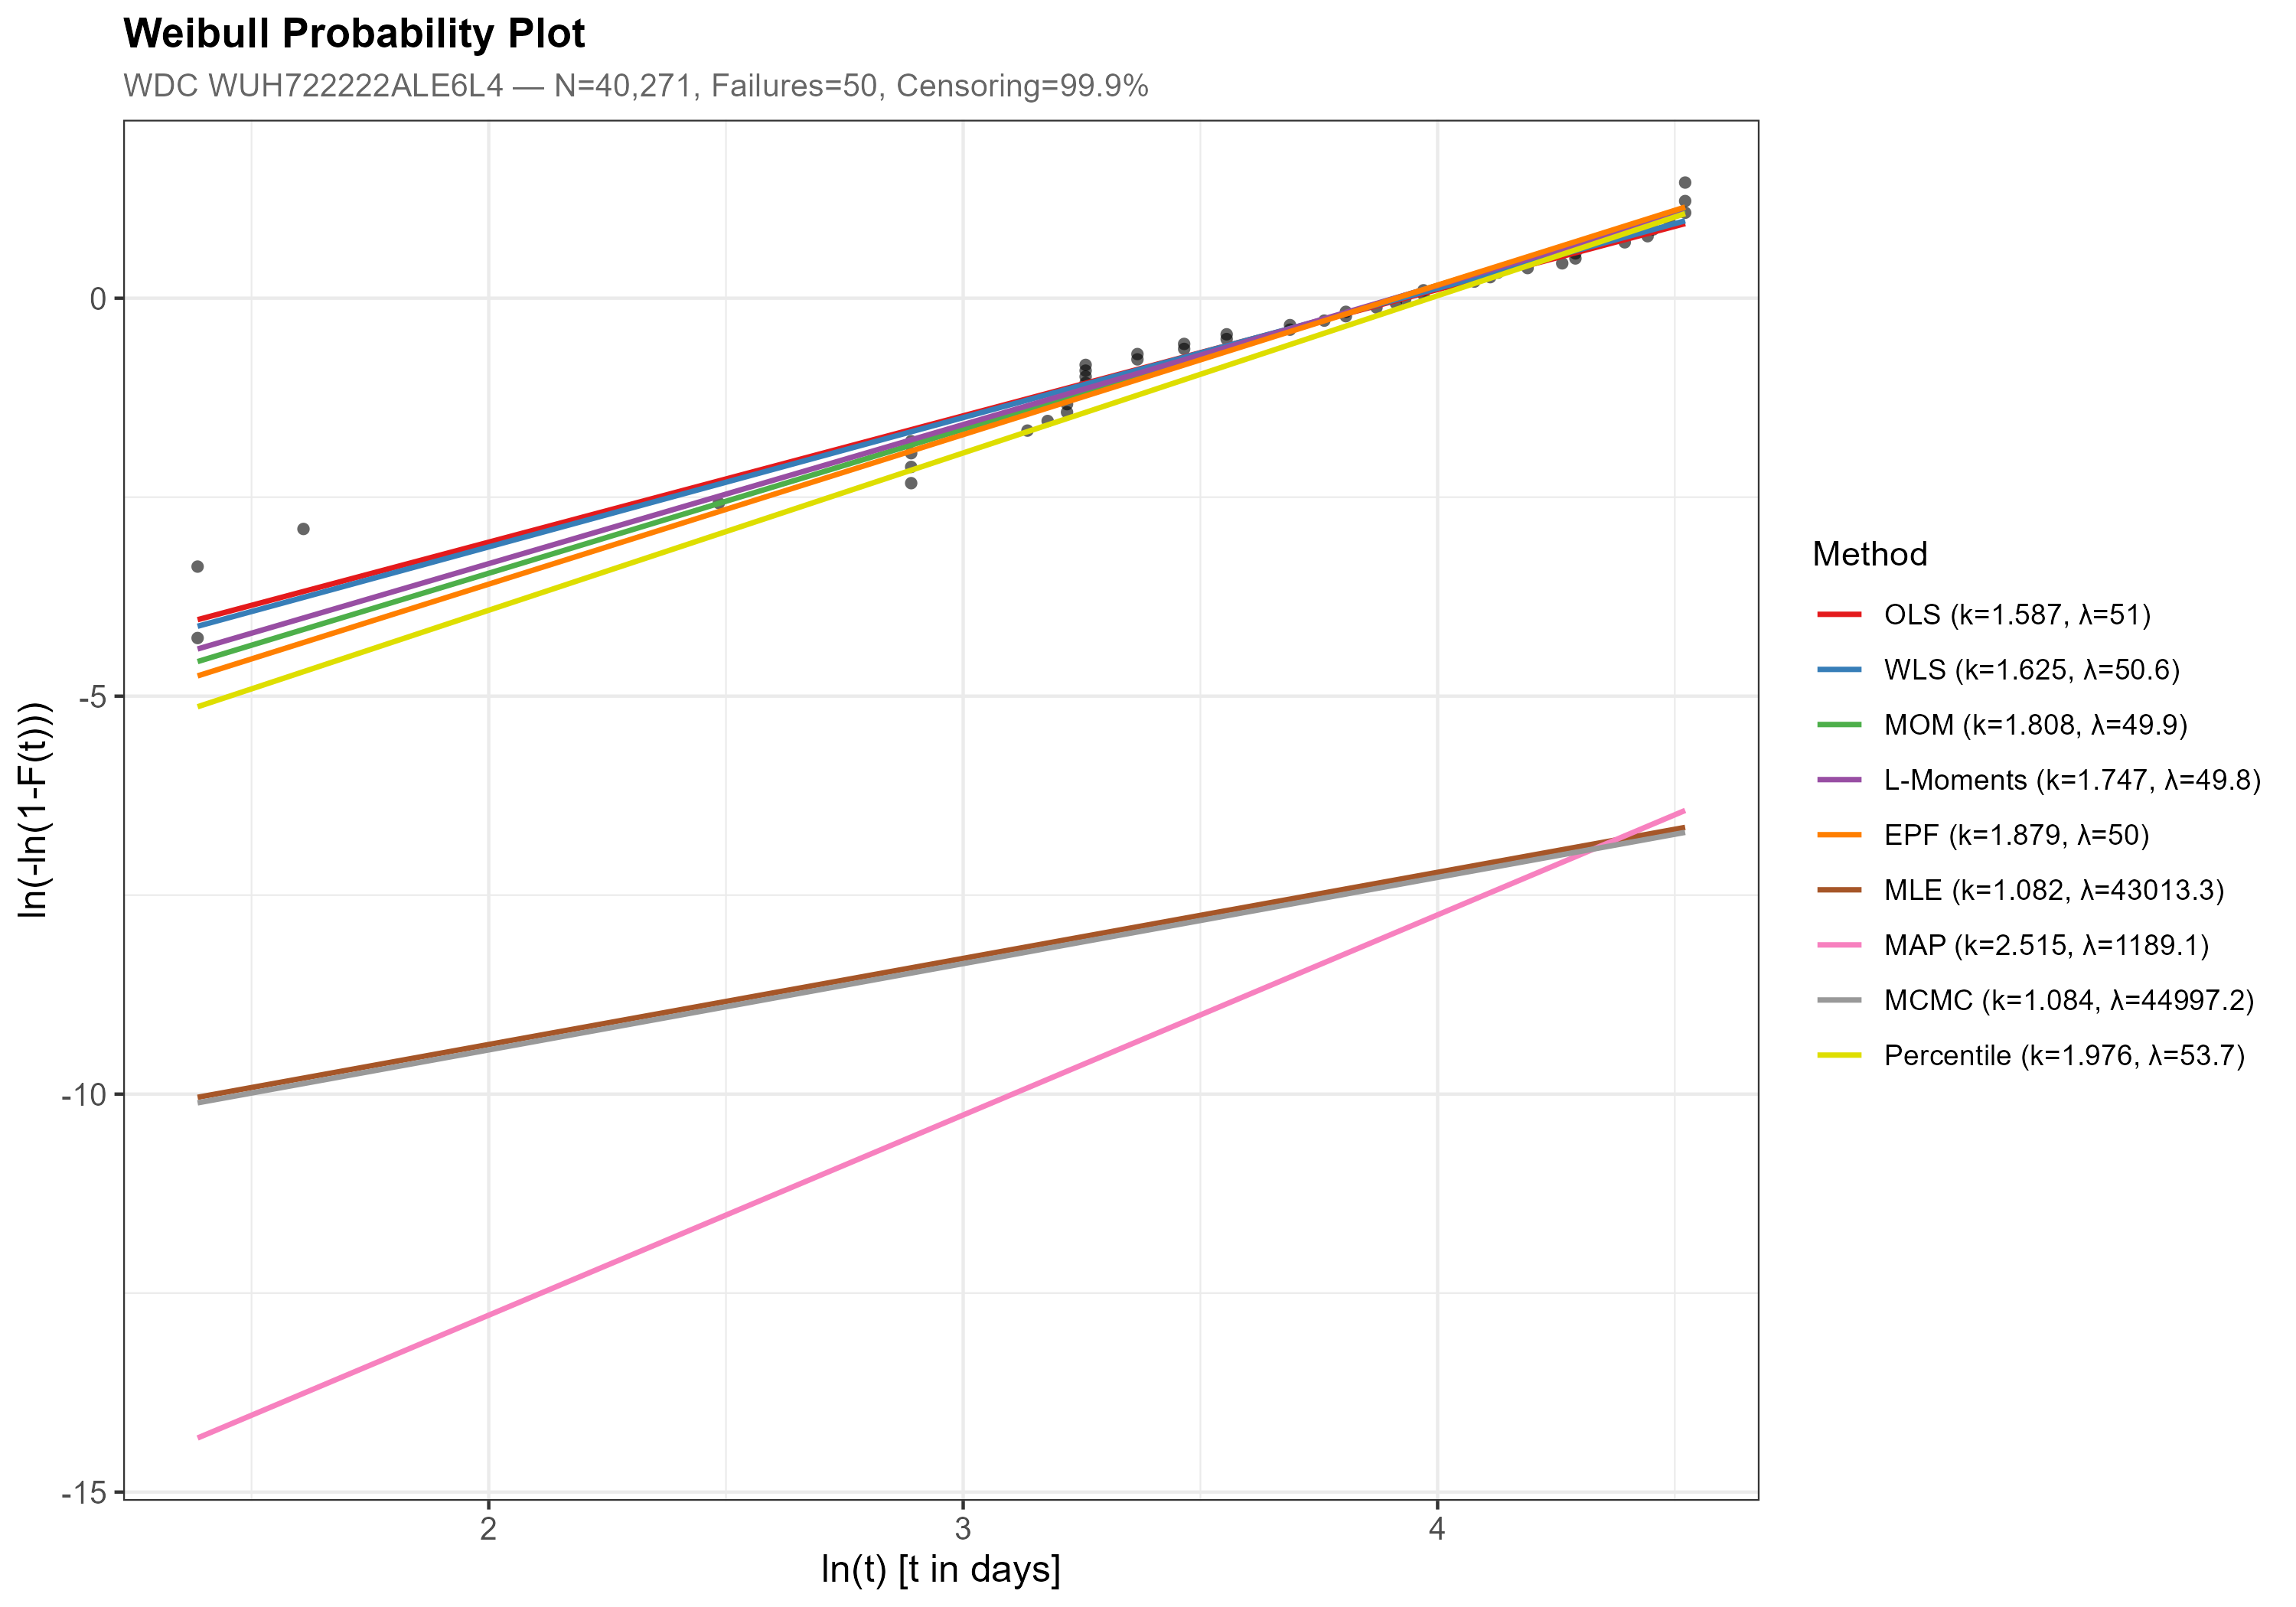
\includegraphics[width=0.95\linewidth]{results/plots/plot1_weibull_probability_WDC_WUH722222ALE6L4.png}
\caption{plot1 weibull probability — WDC WUH722222ALE6L4}
\end{figure}

\begin{figure}[H]
\centering
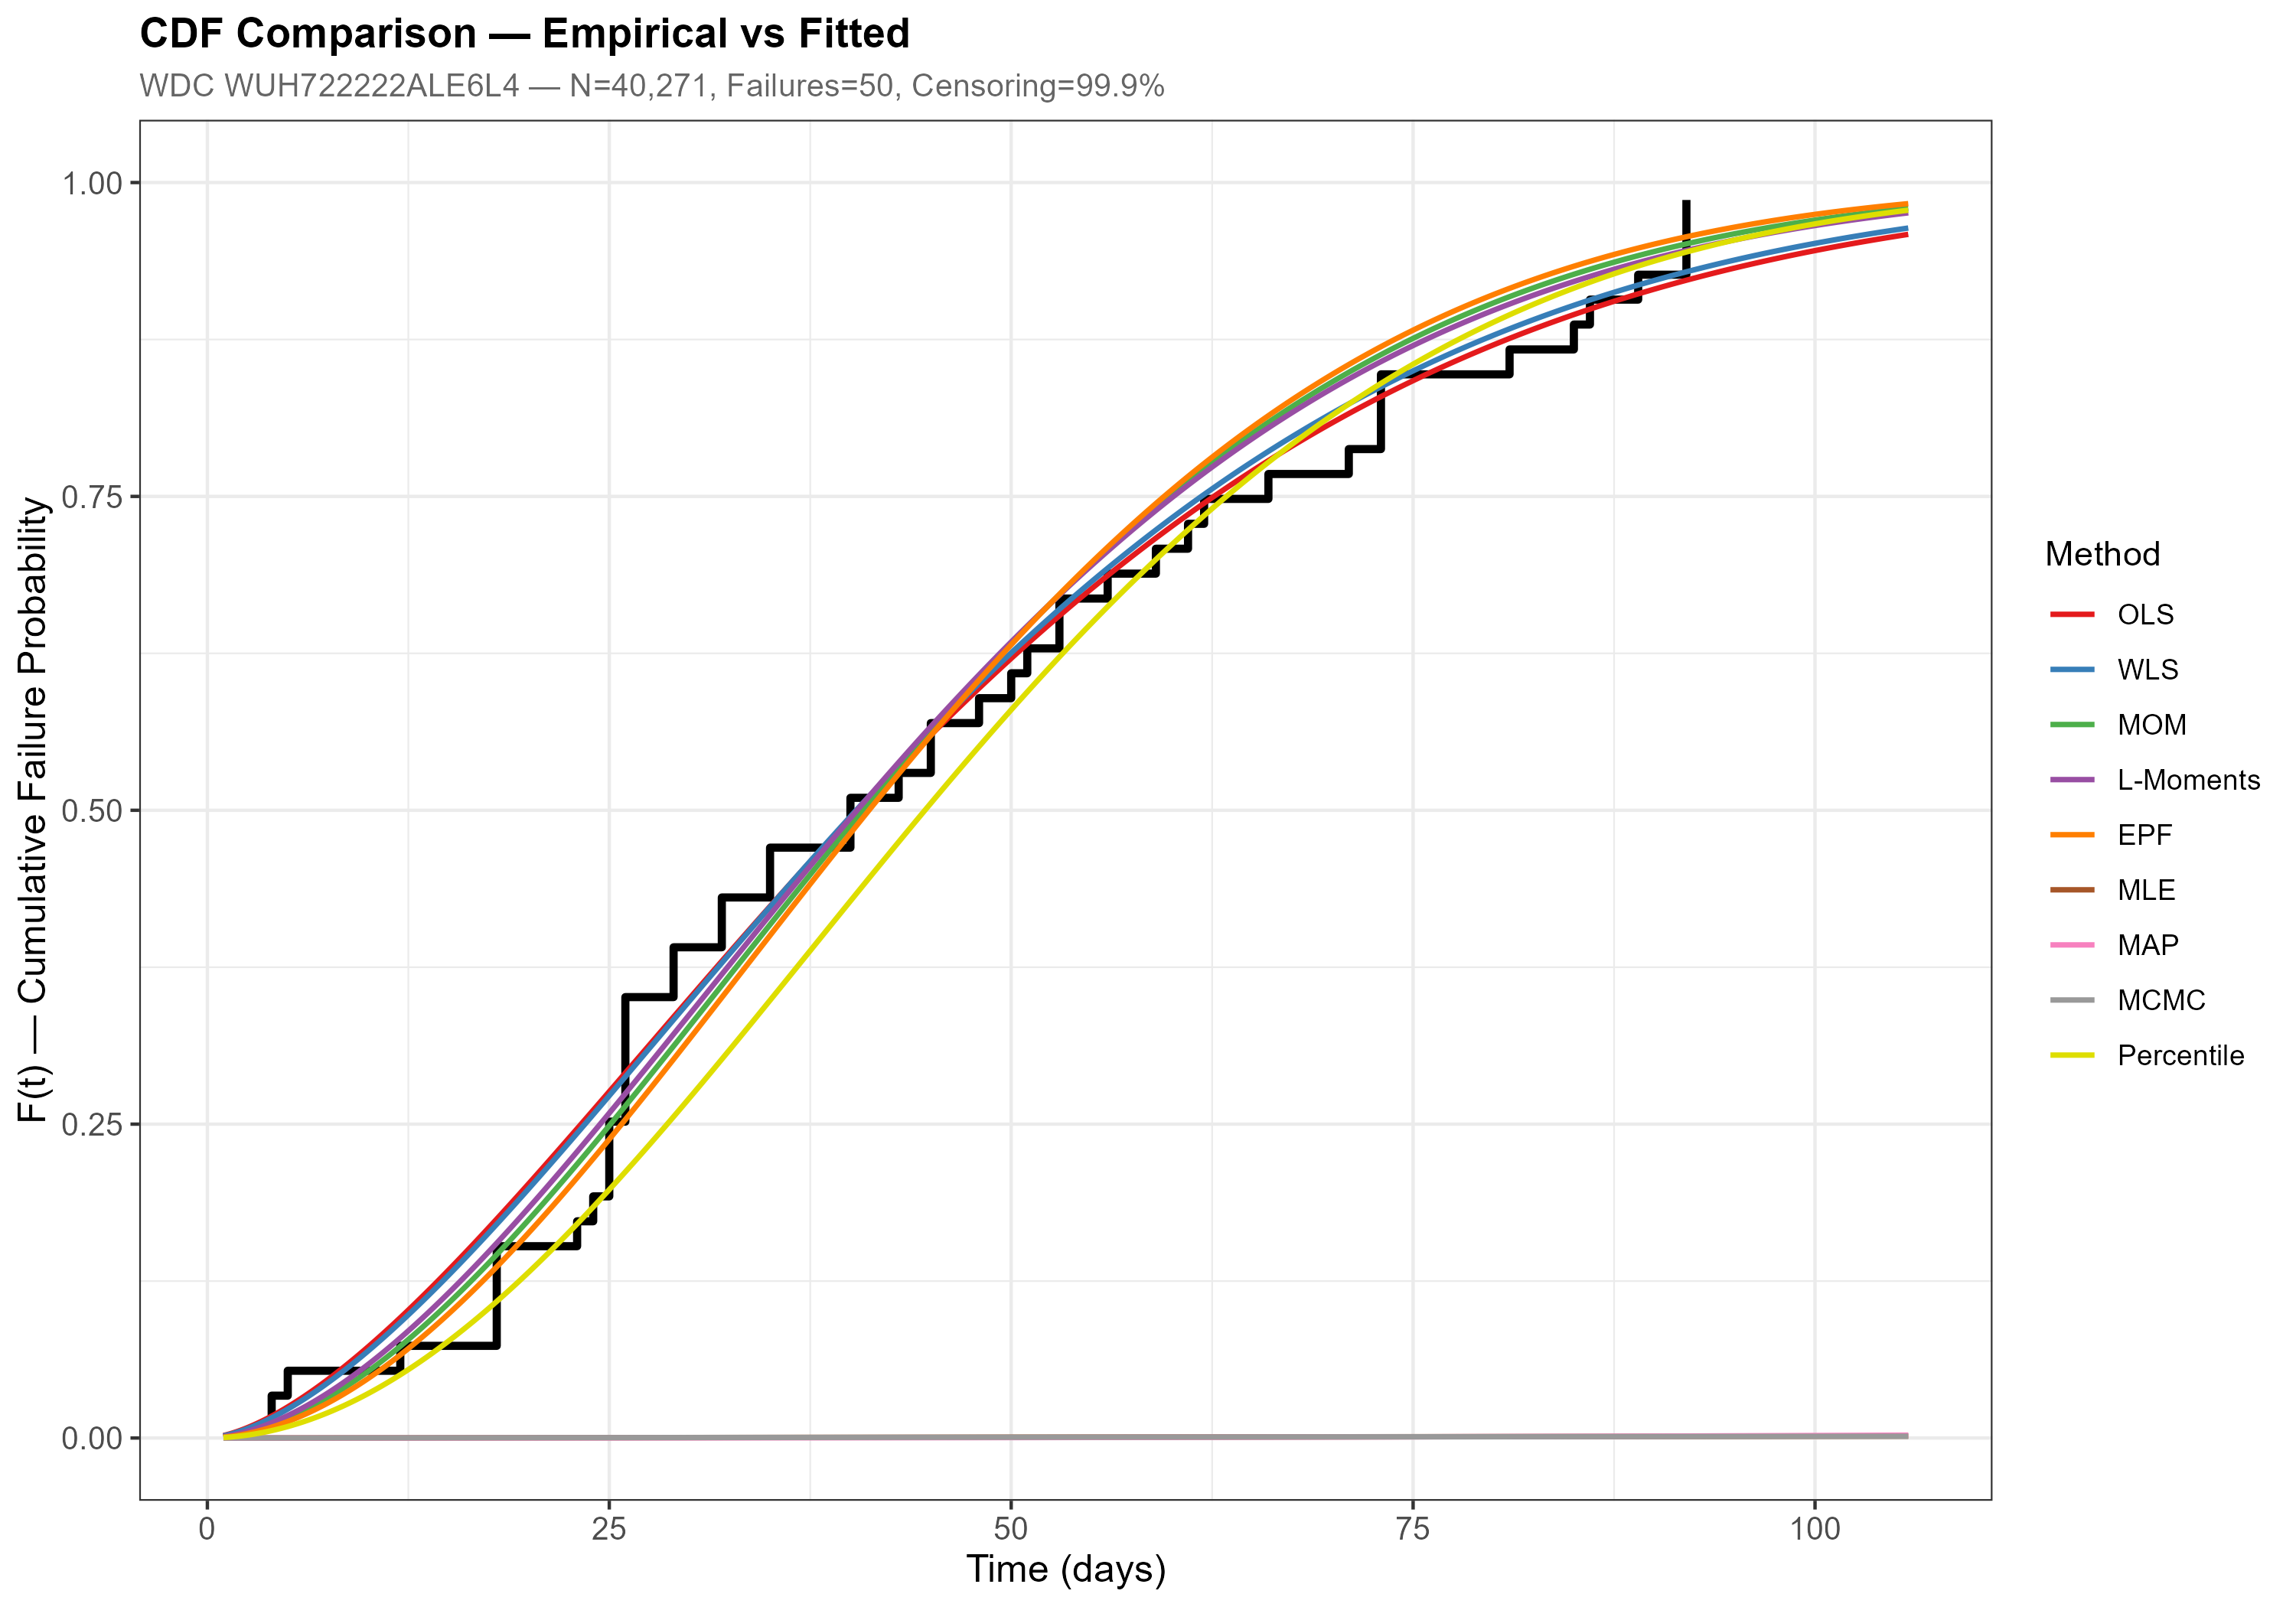
\includegraphics[width=0.95\linewidth]{results/plots/plot2_cdf_WDC_WUH722222ALE6L4.png}
\caption{plot2 cdf — WDC WUH722222ALE6L4}
\end{figure}

\begin{figure}[H]
\centering
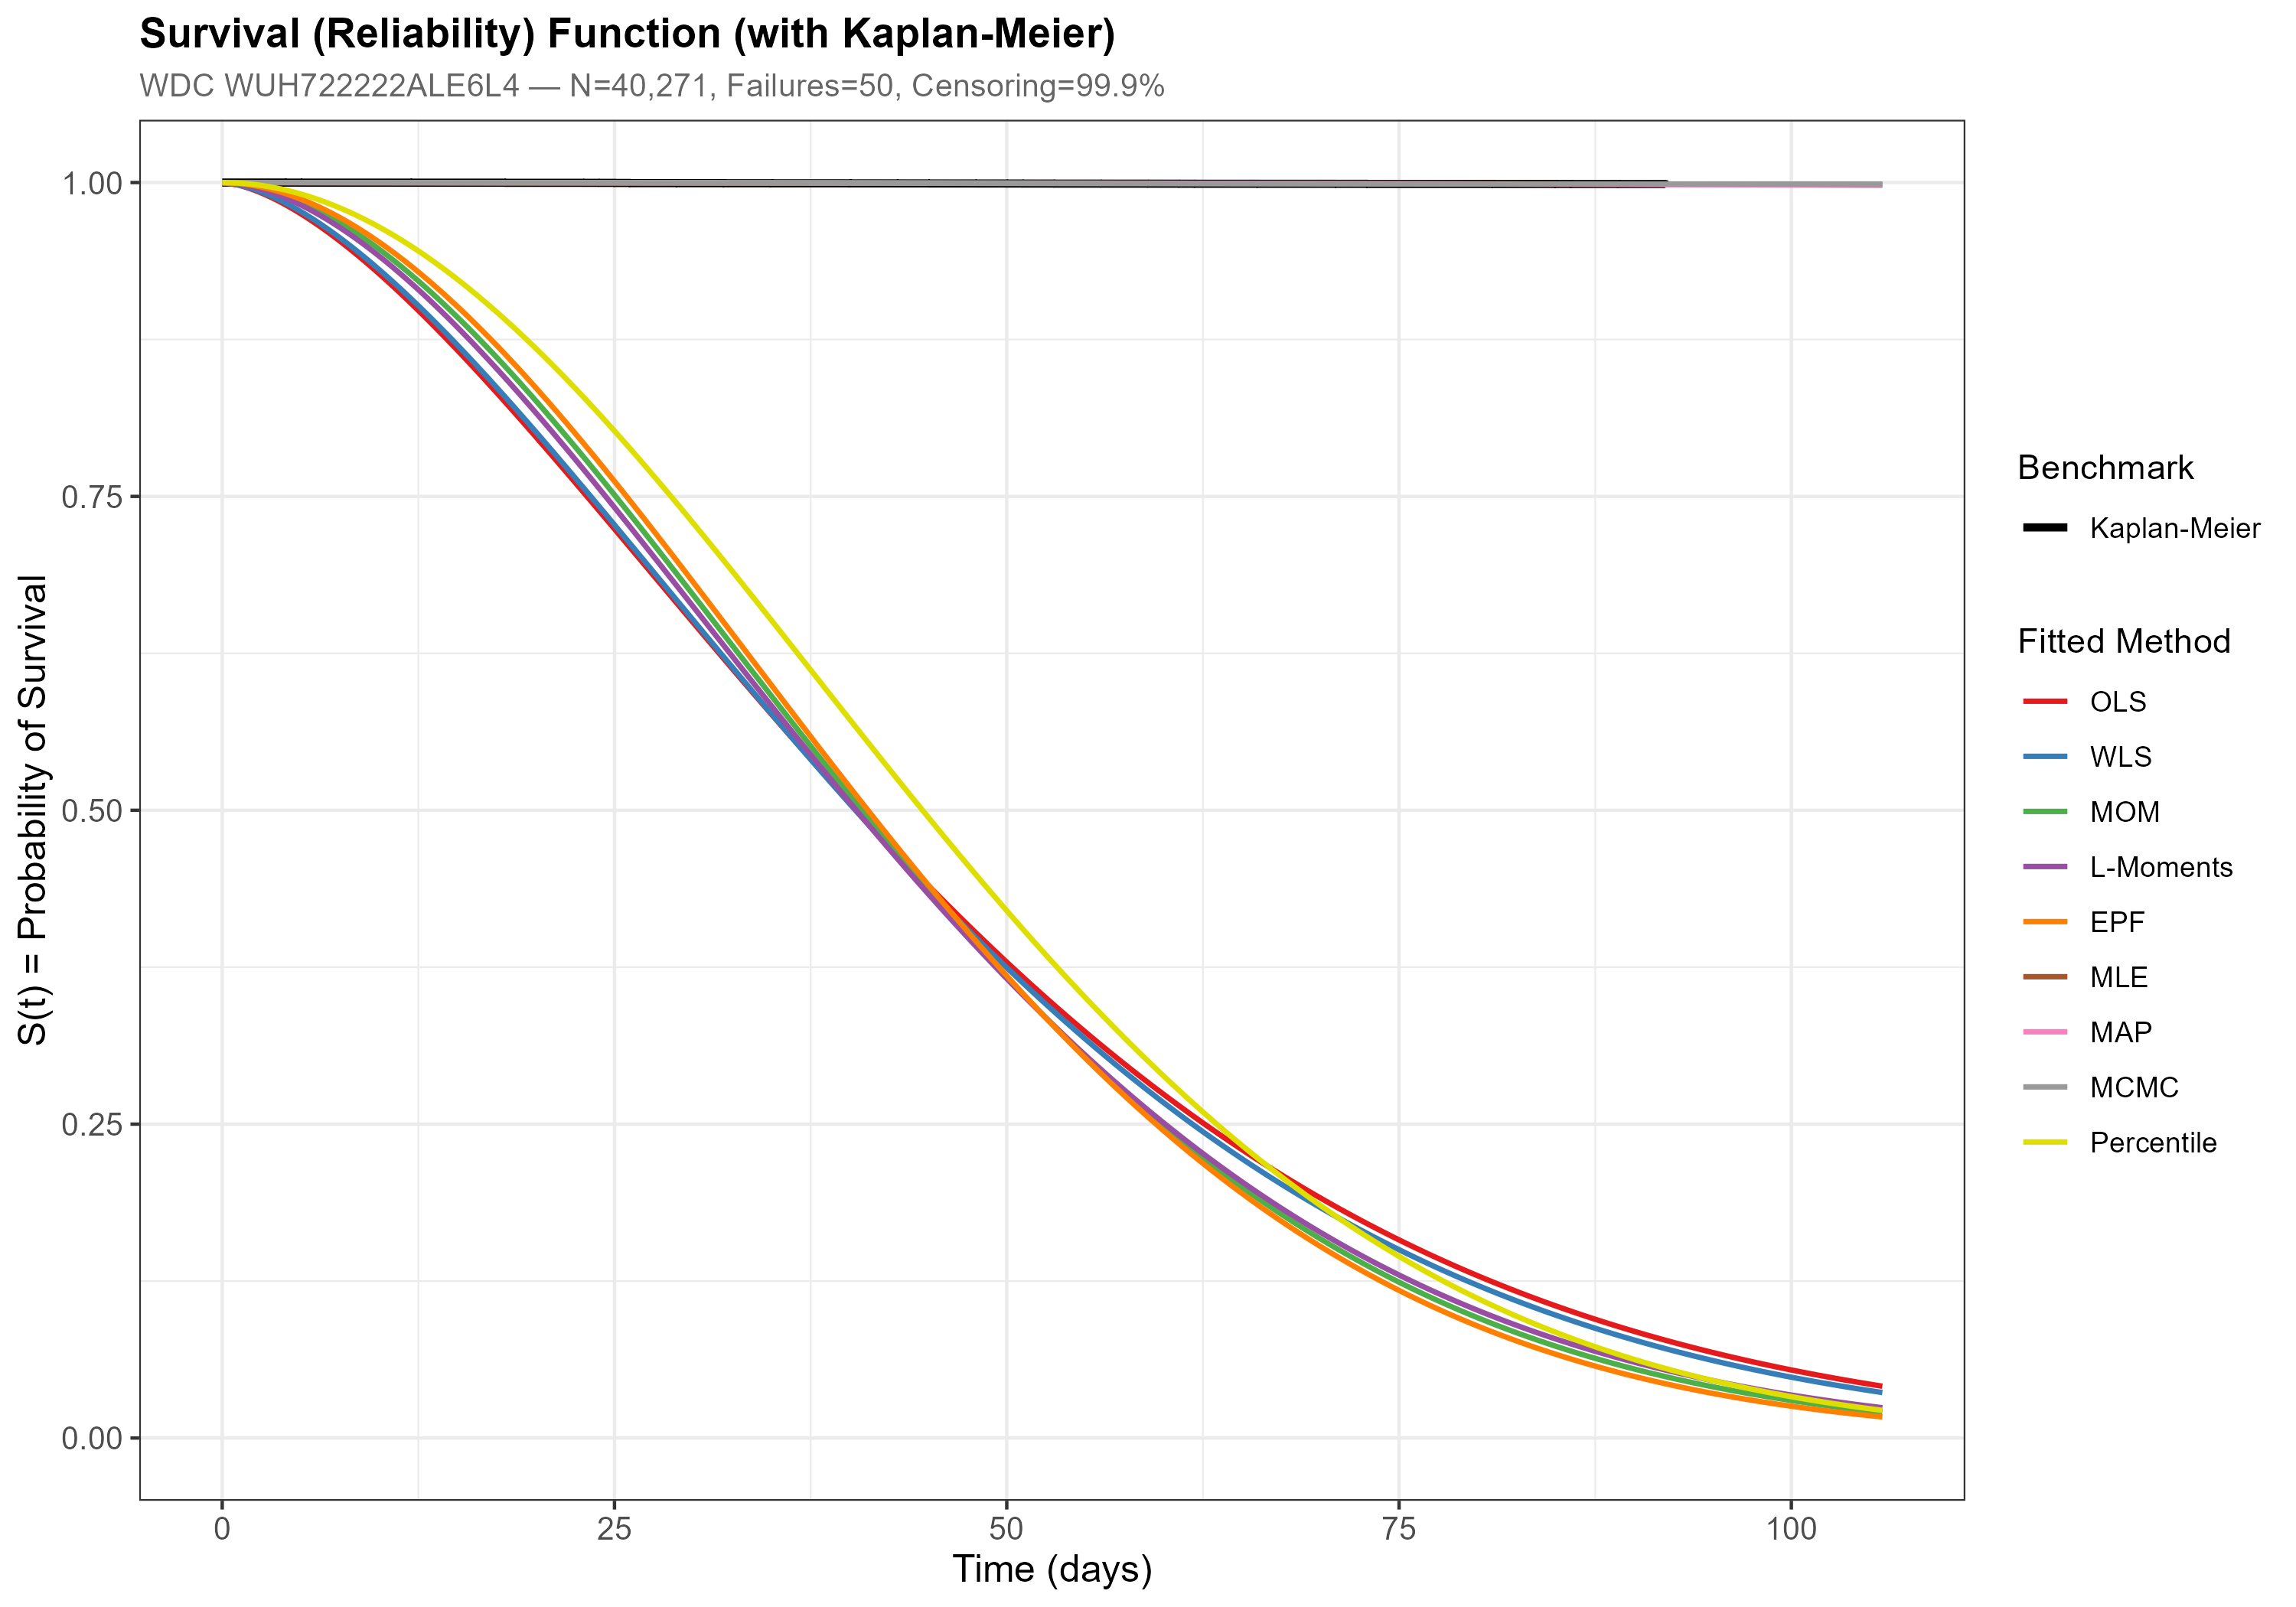
\includegraphics[width=0.95\linewidth]{results/plots/plot3_survival_WDC_WUH722222ALE6L4.png}
\caption{plot3 survival — WDC WUH722222ALE6L4}
\end{figure}

\begin{figure}[H]
\centering
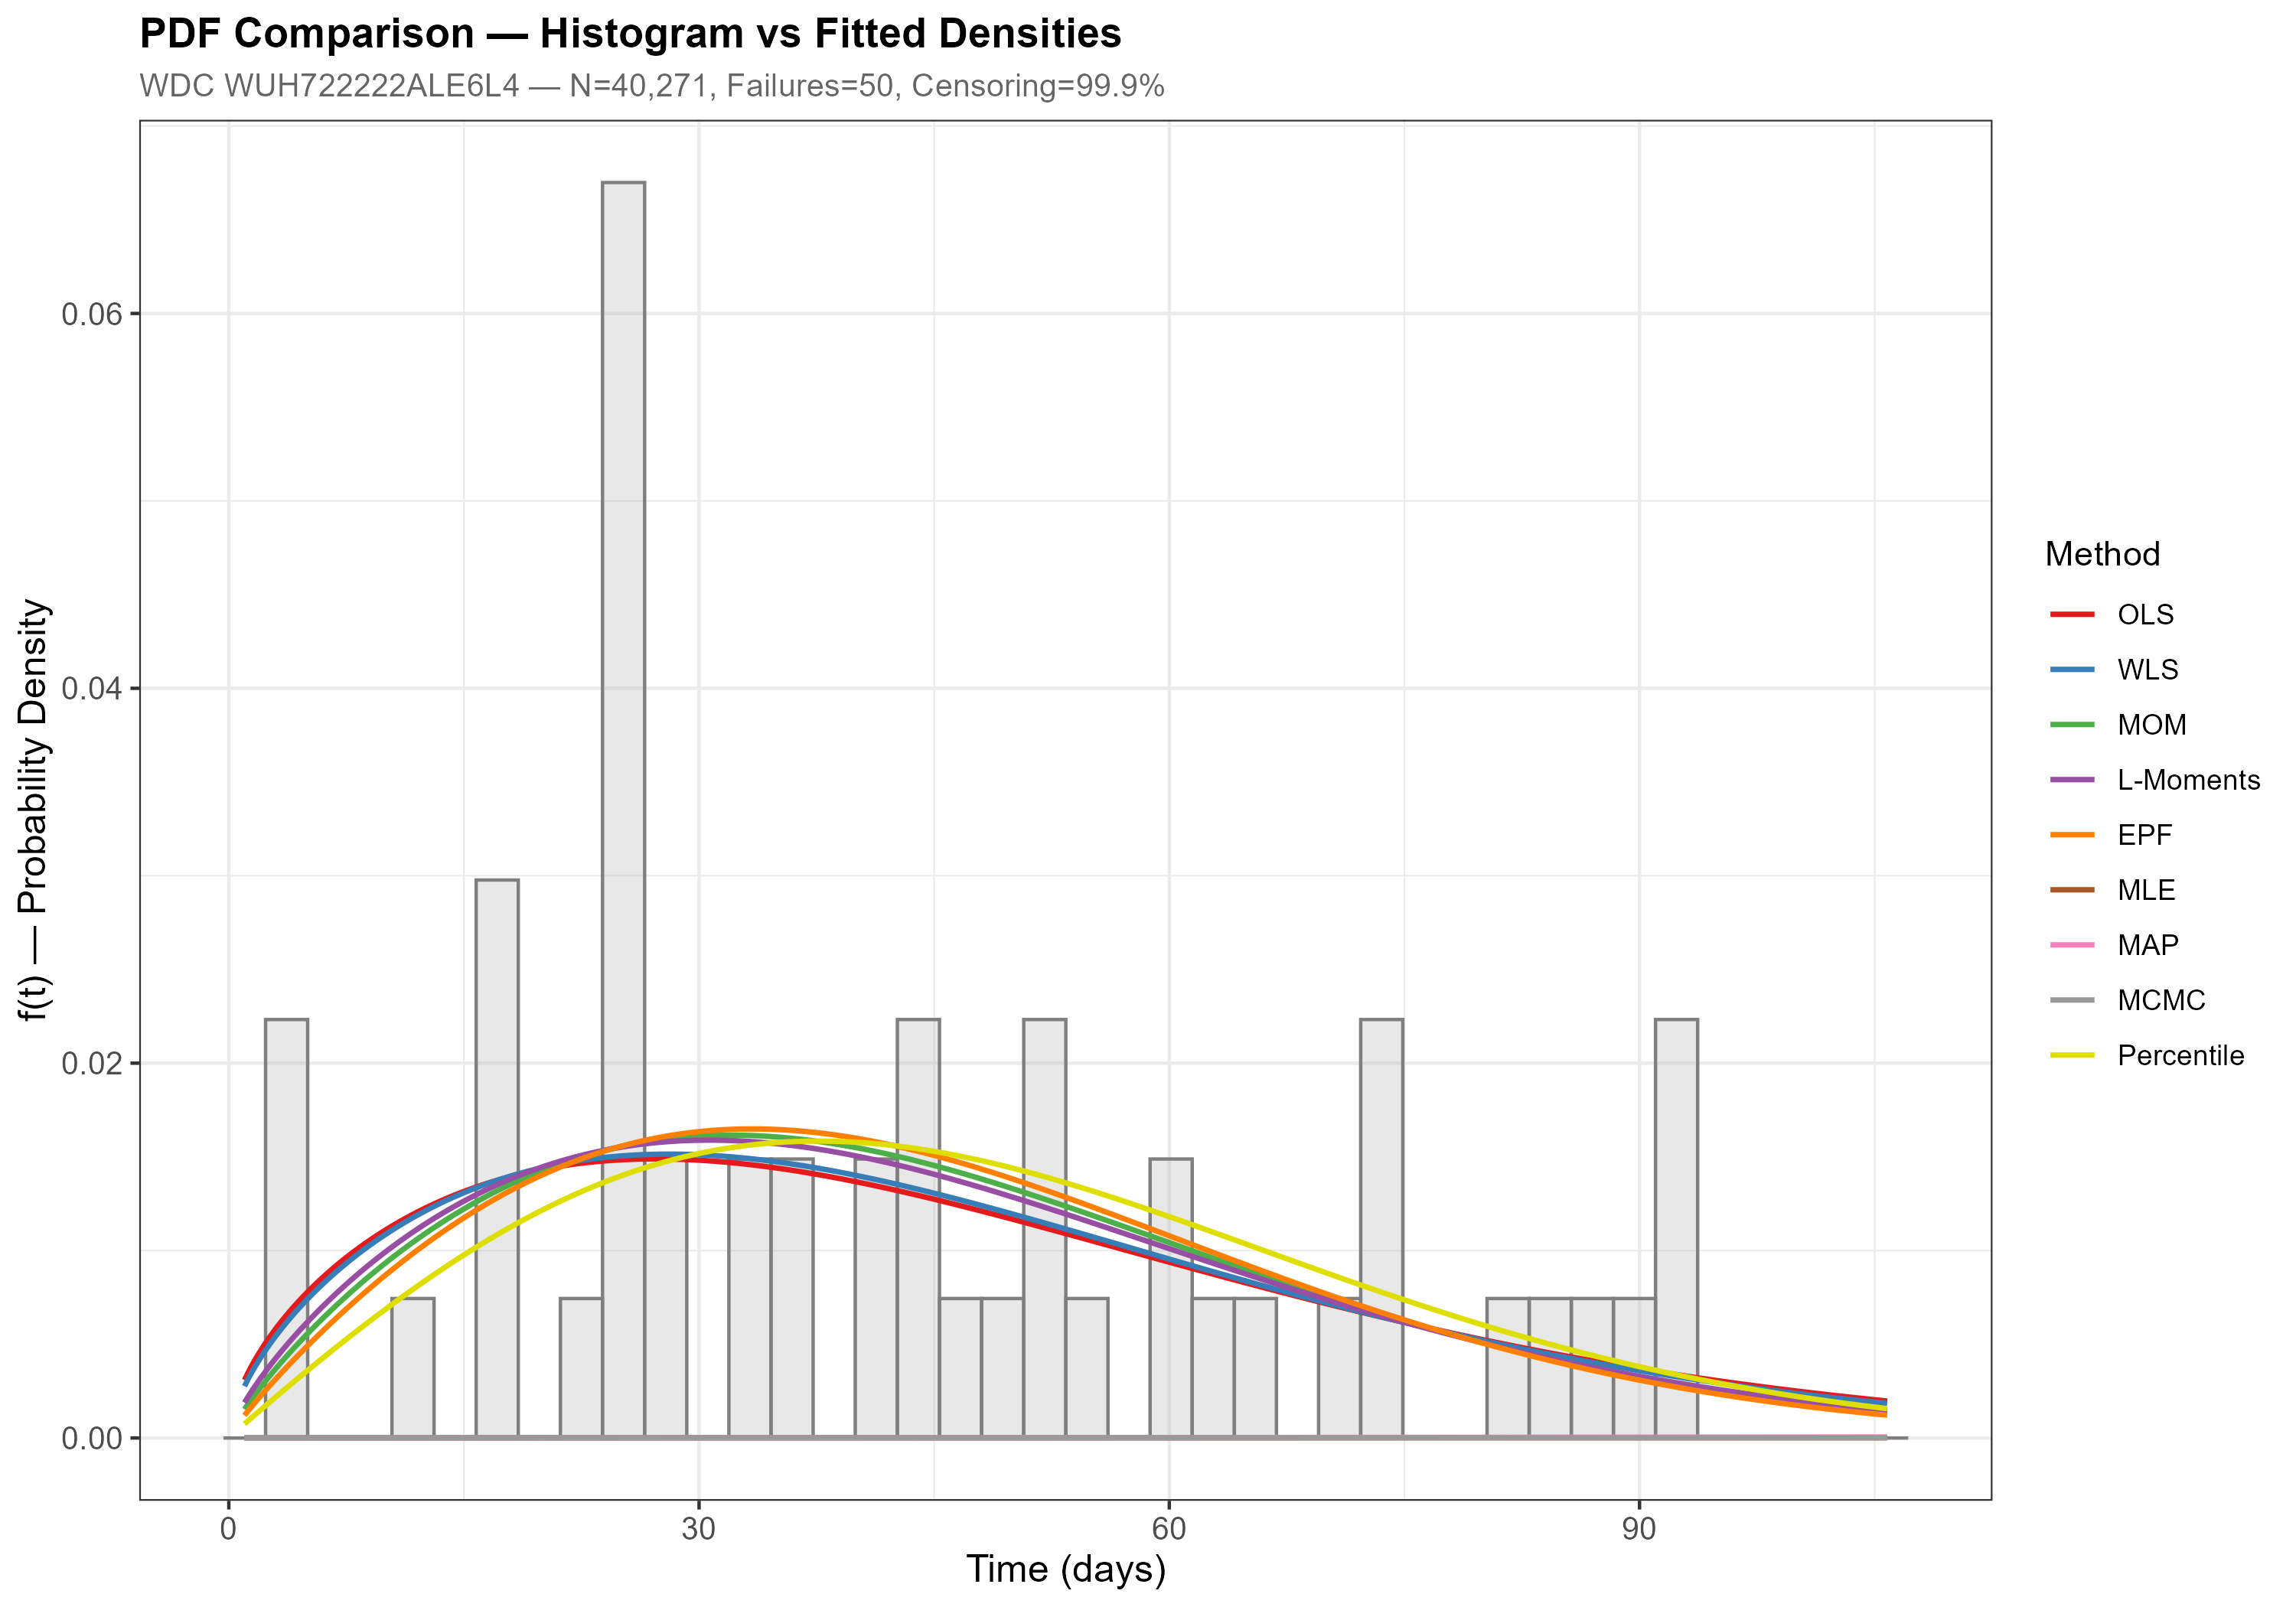
\includegraphics[width=0.95\linewidth]{results/plots/plot4_pdf_WDC_WUH722222ALE6L4.png}
\caption{plot4 pdf — WDC WUH722222ALE6L4}
\end{figure}

\begin{figure}[H]
\centering
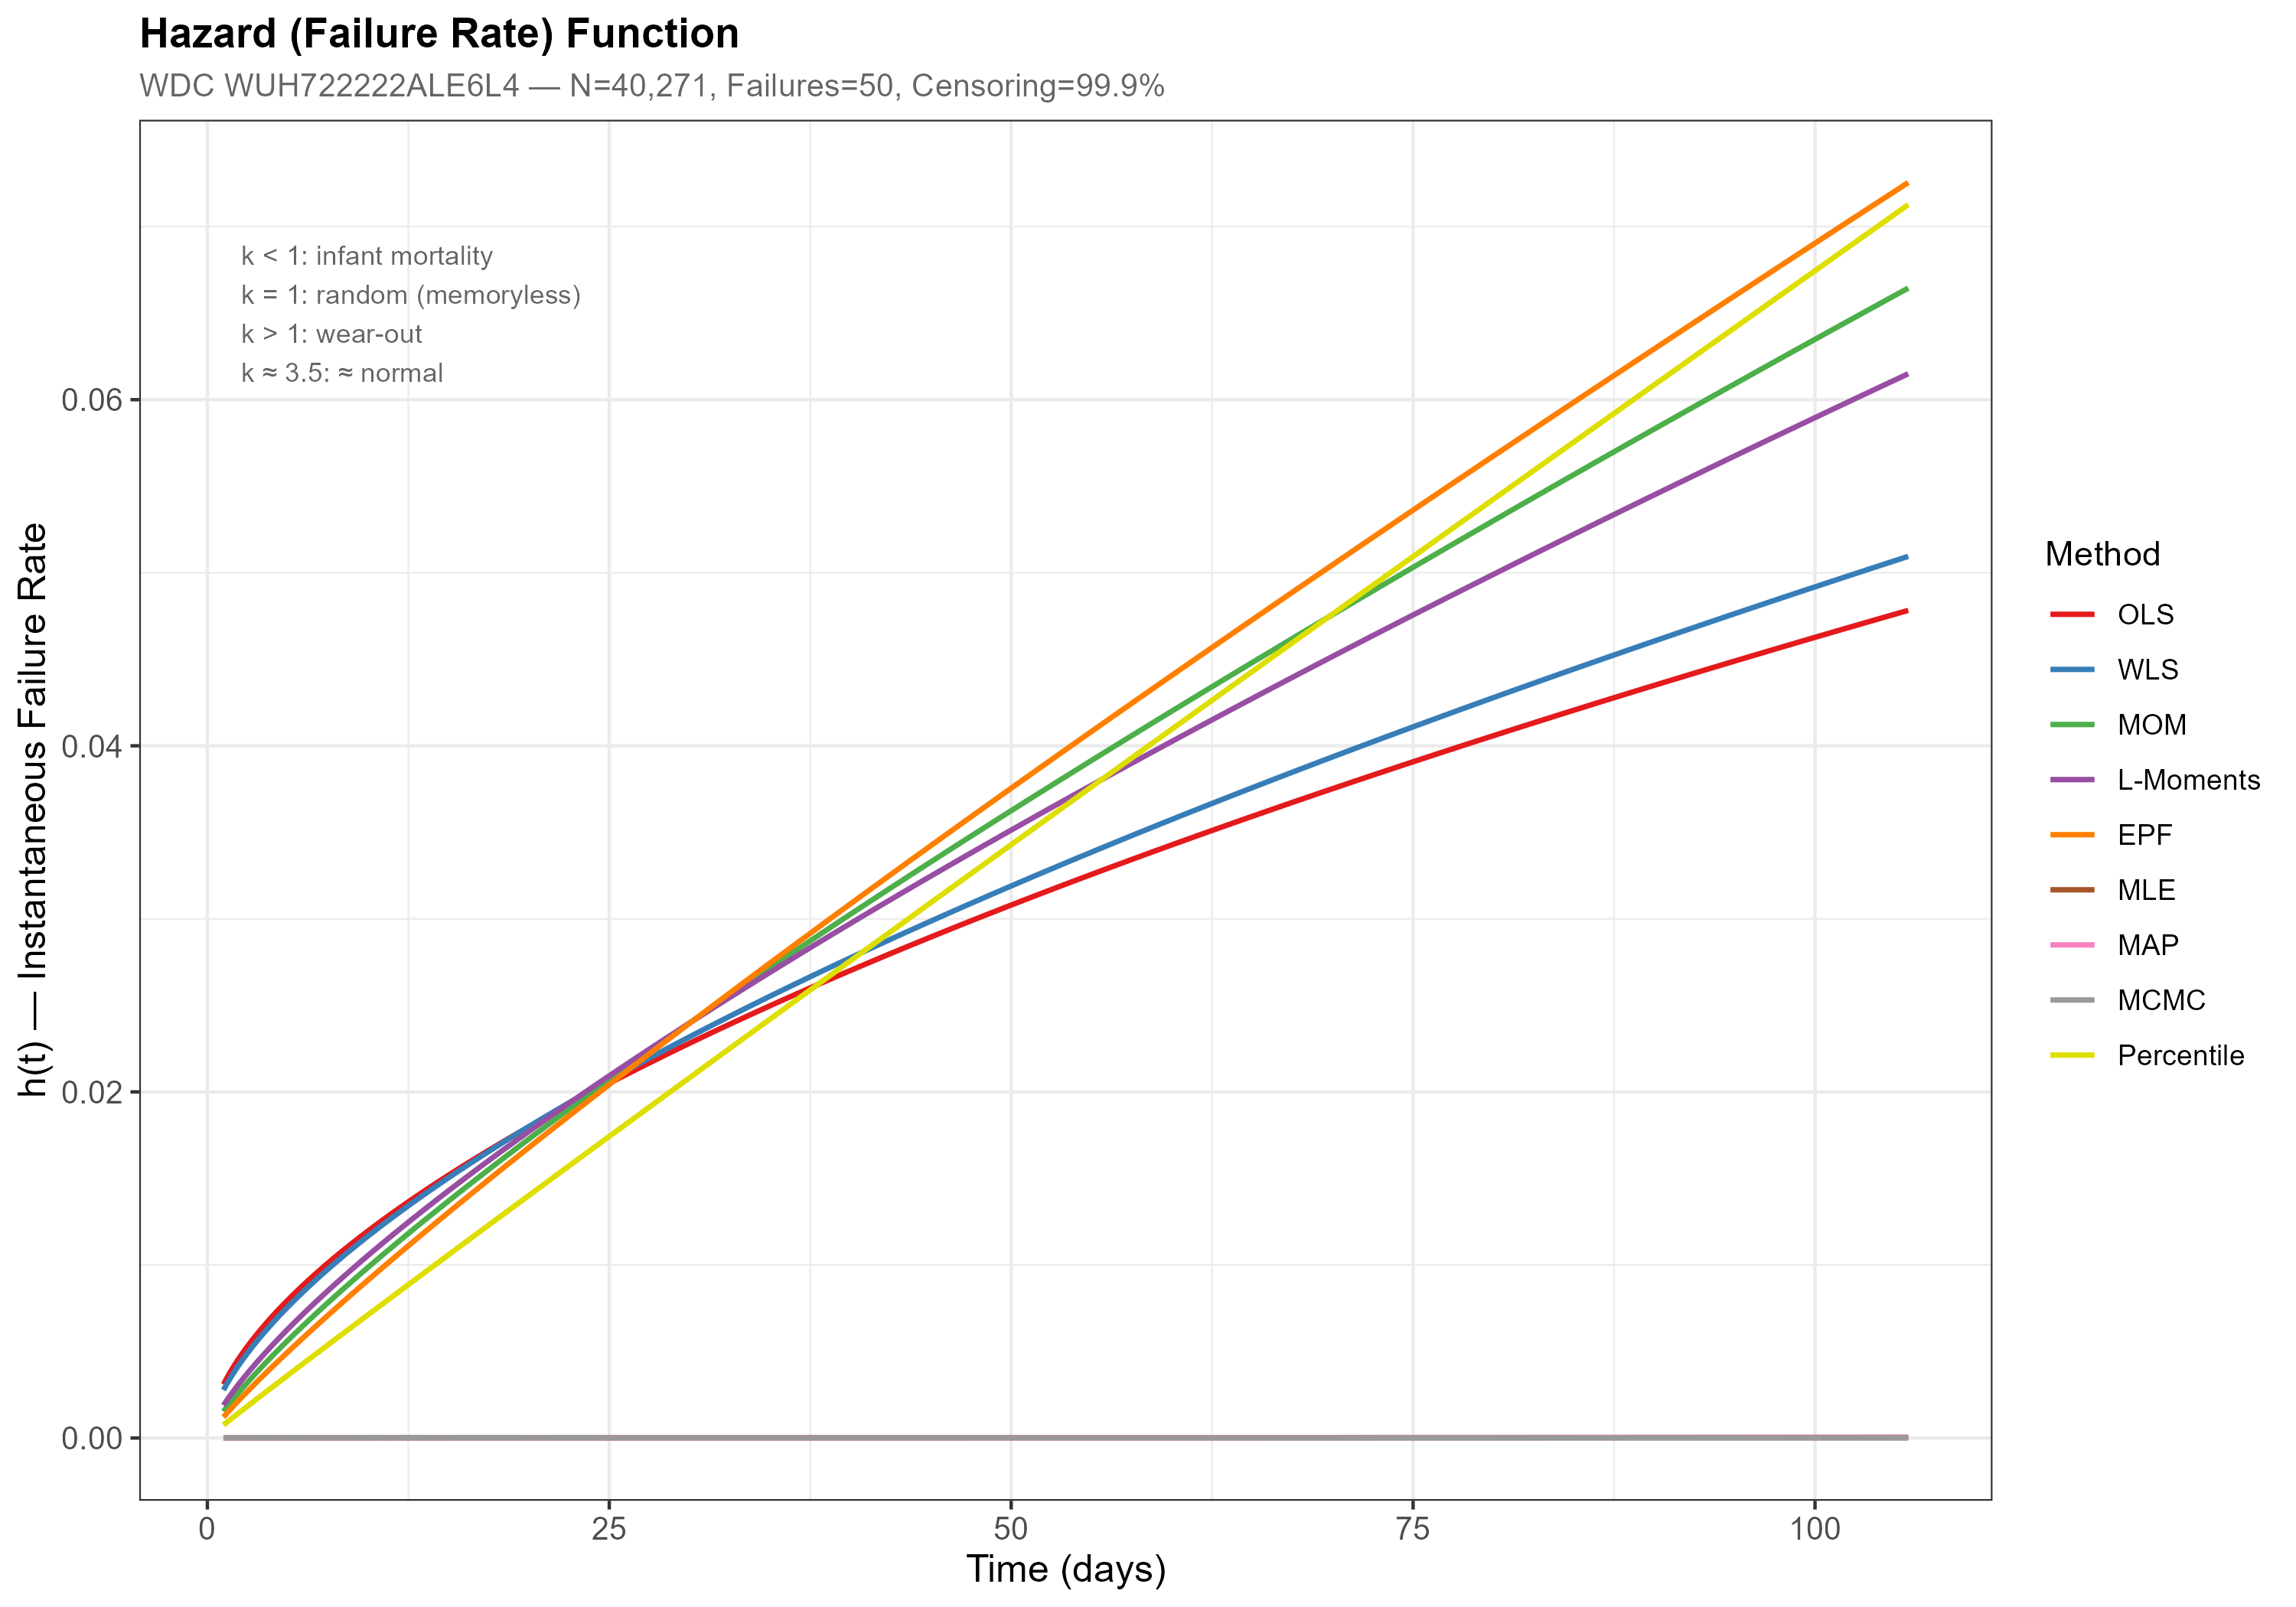
\includegraphics[width=0.95\linewidth]{results/plots/plot5_hazard_WDC_WUH722222ALE6L4.png}
\caption{plot5 hazard — WDC WUH722222ALE6L4}
\end{figure}

\begin{figure}[H]
\centering
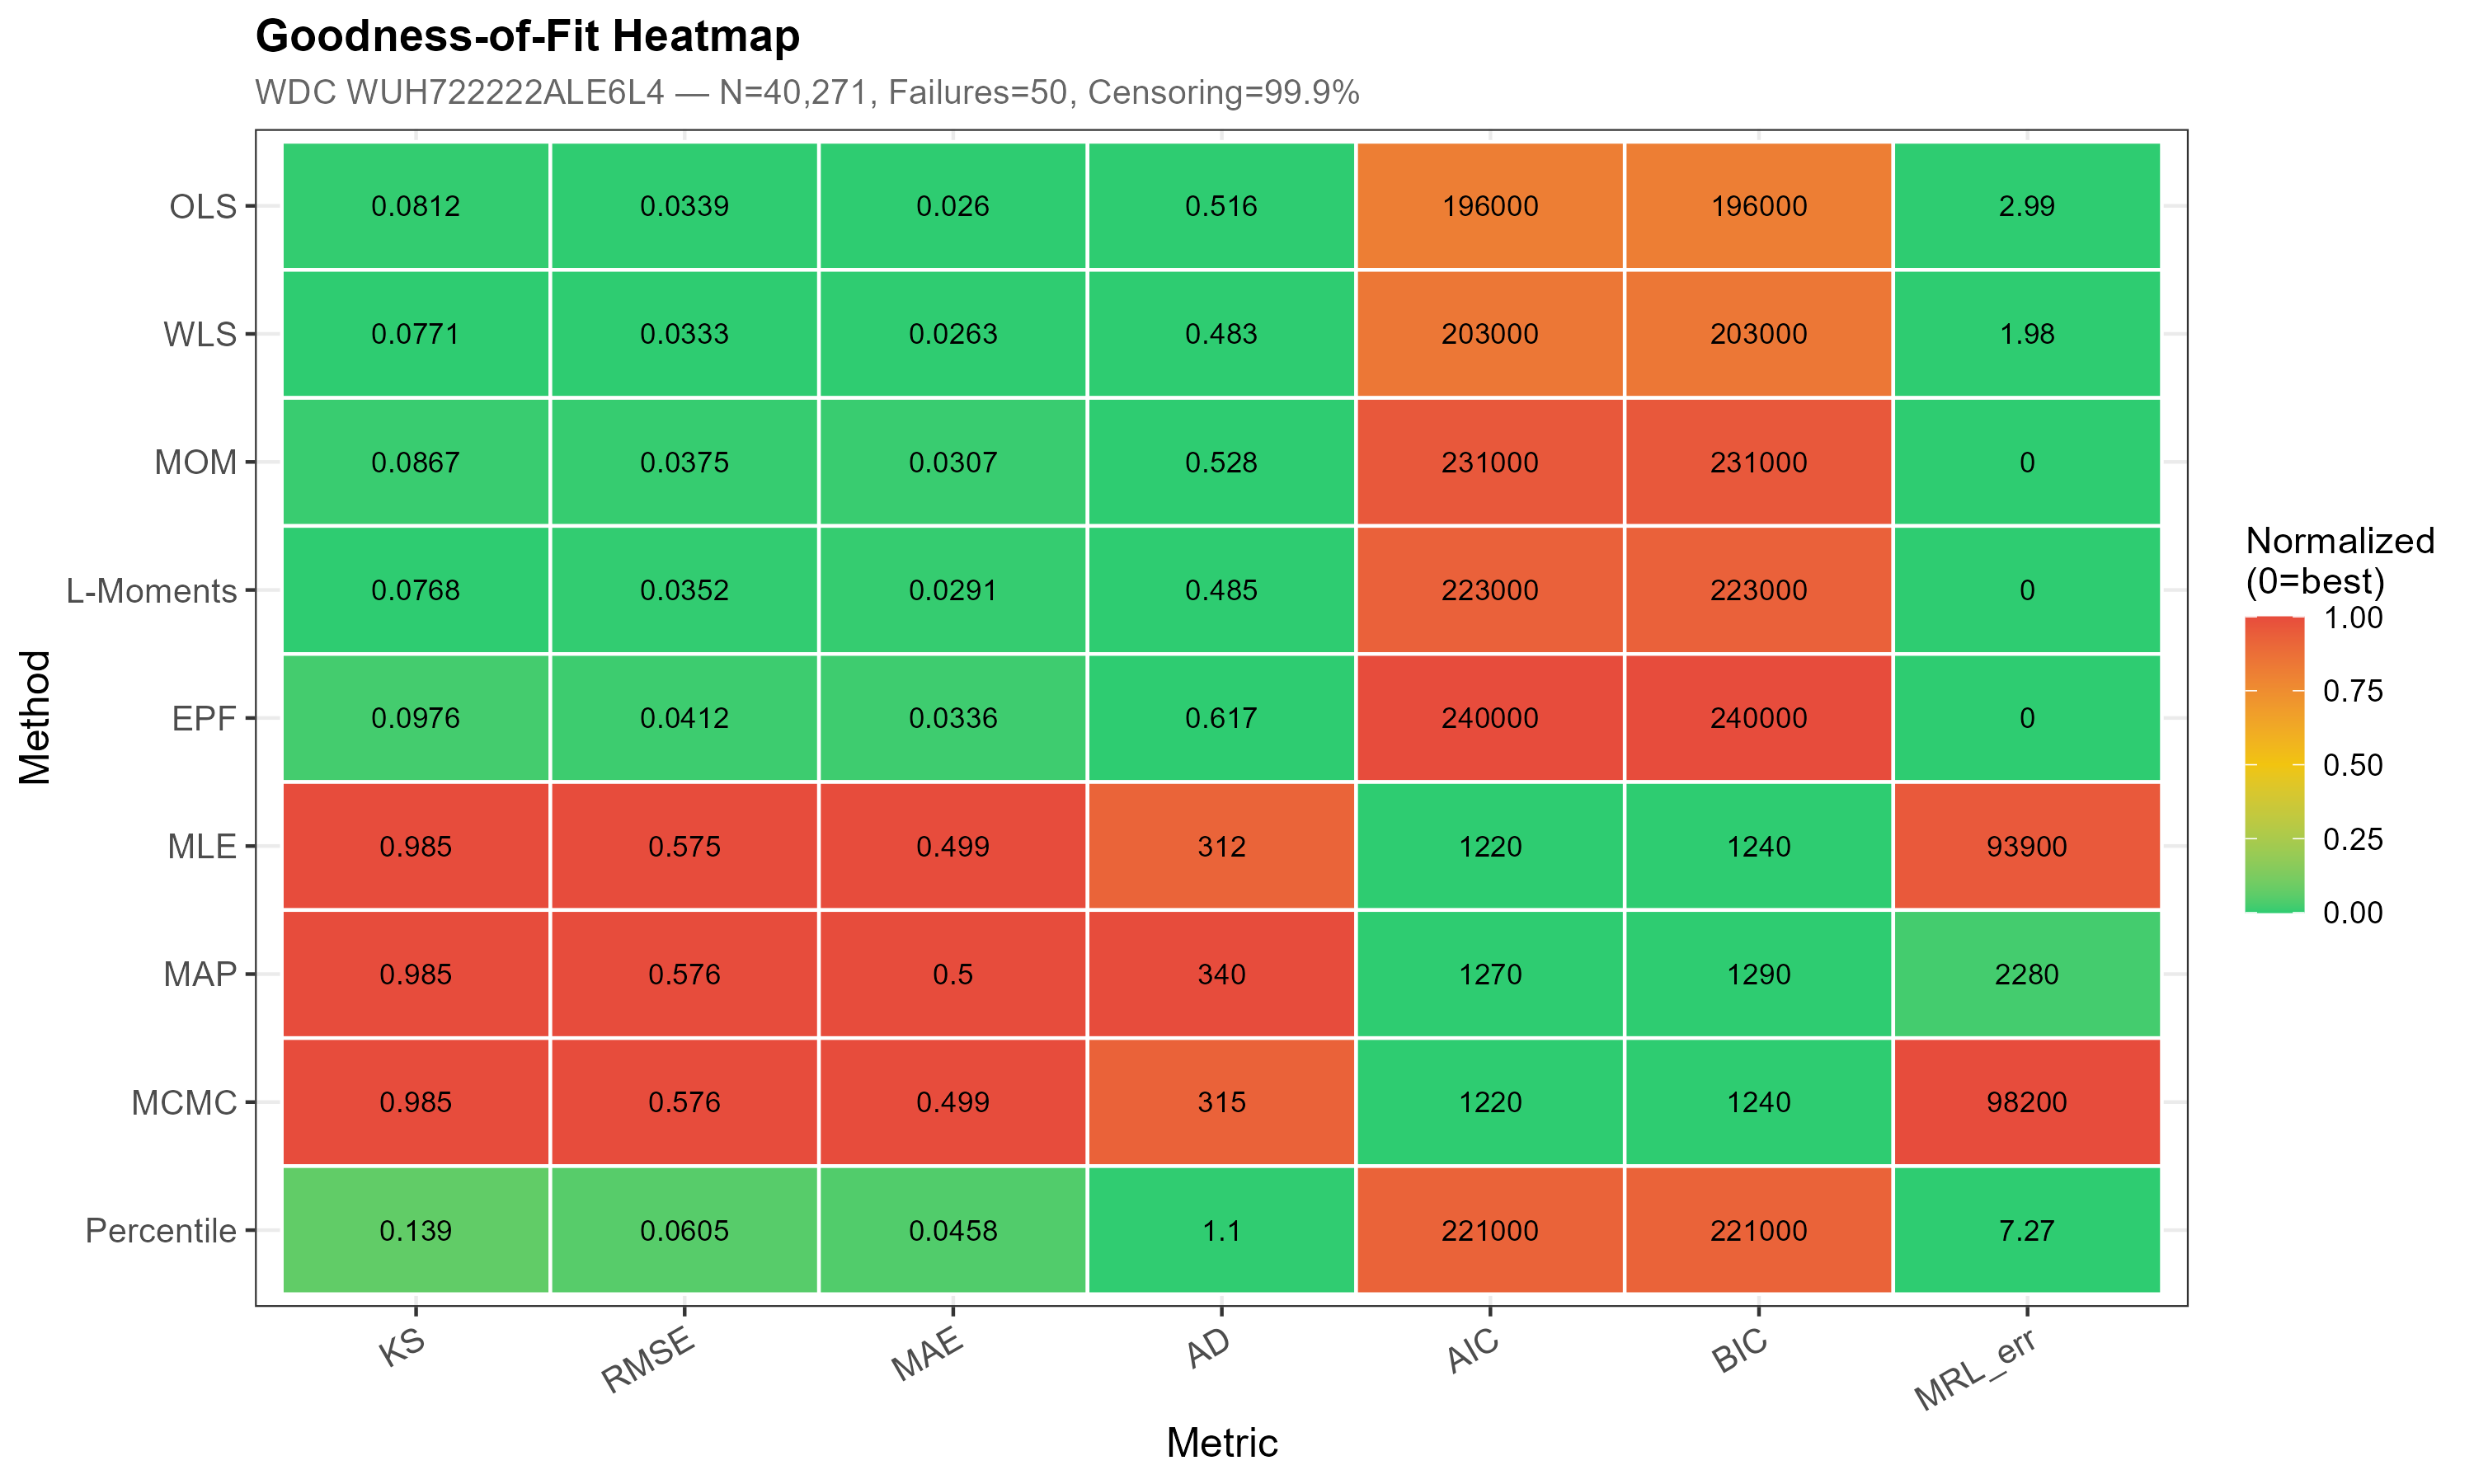
\includegraphics[width=0.95\linewidth]{results/plots/plot6_gof_heatmap_WDC_WUH722222ALE6L4.png}
\caption{plot6 gof heatmap — WDC WUH722222ALE6L4}
\end{figure}

\begin{figure}[H]
\centering
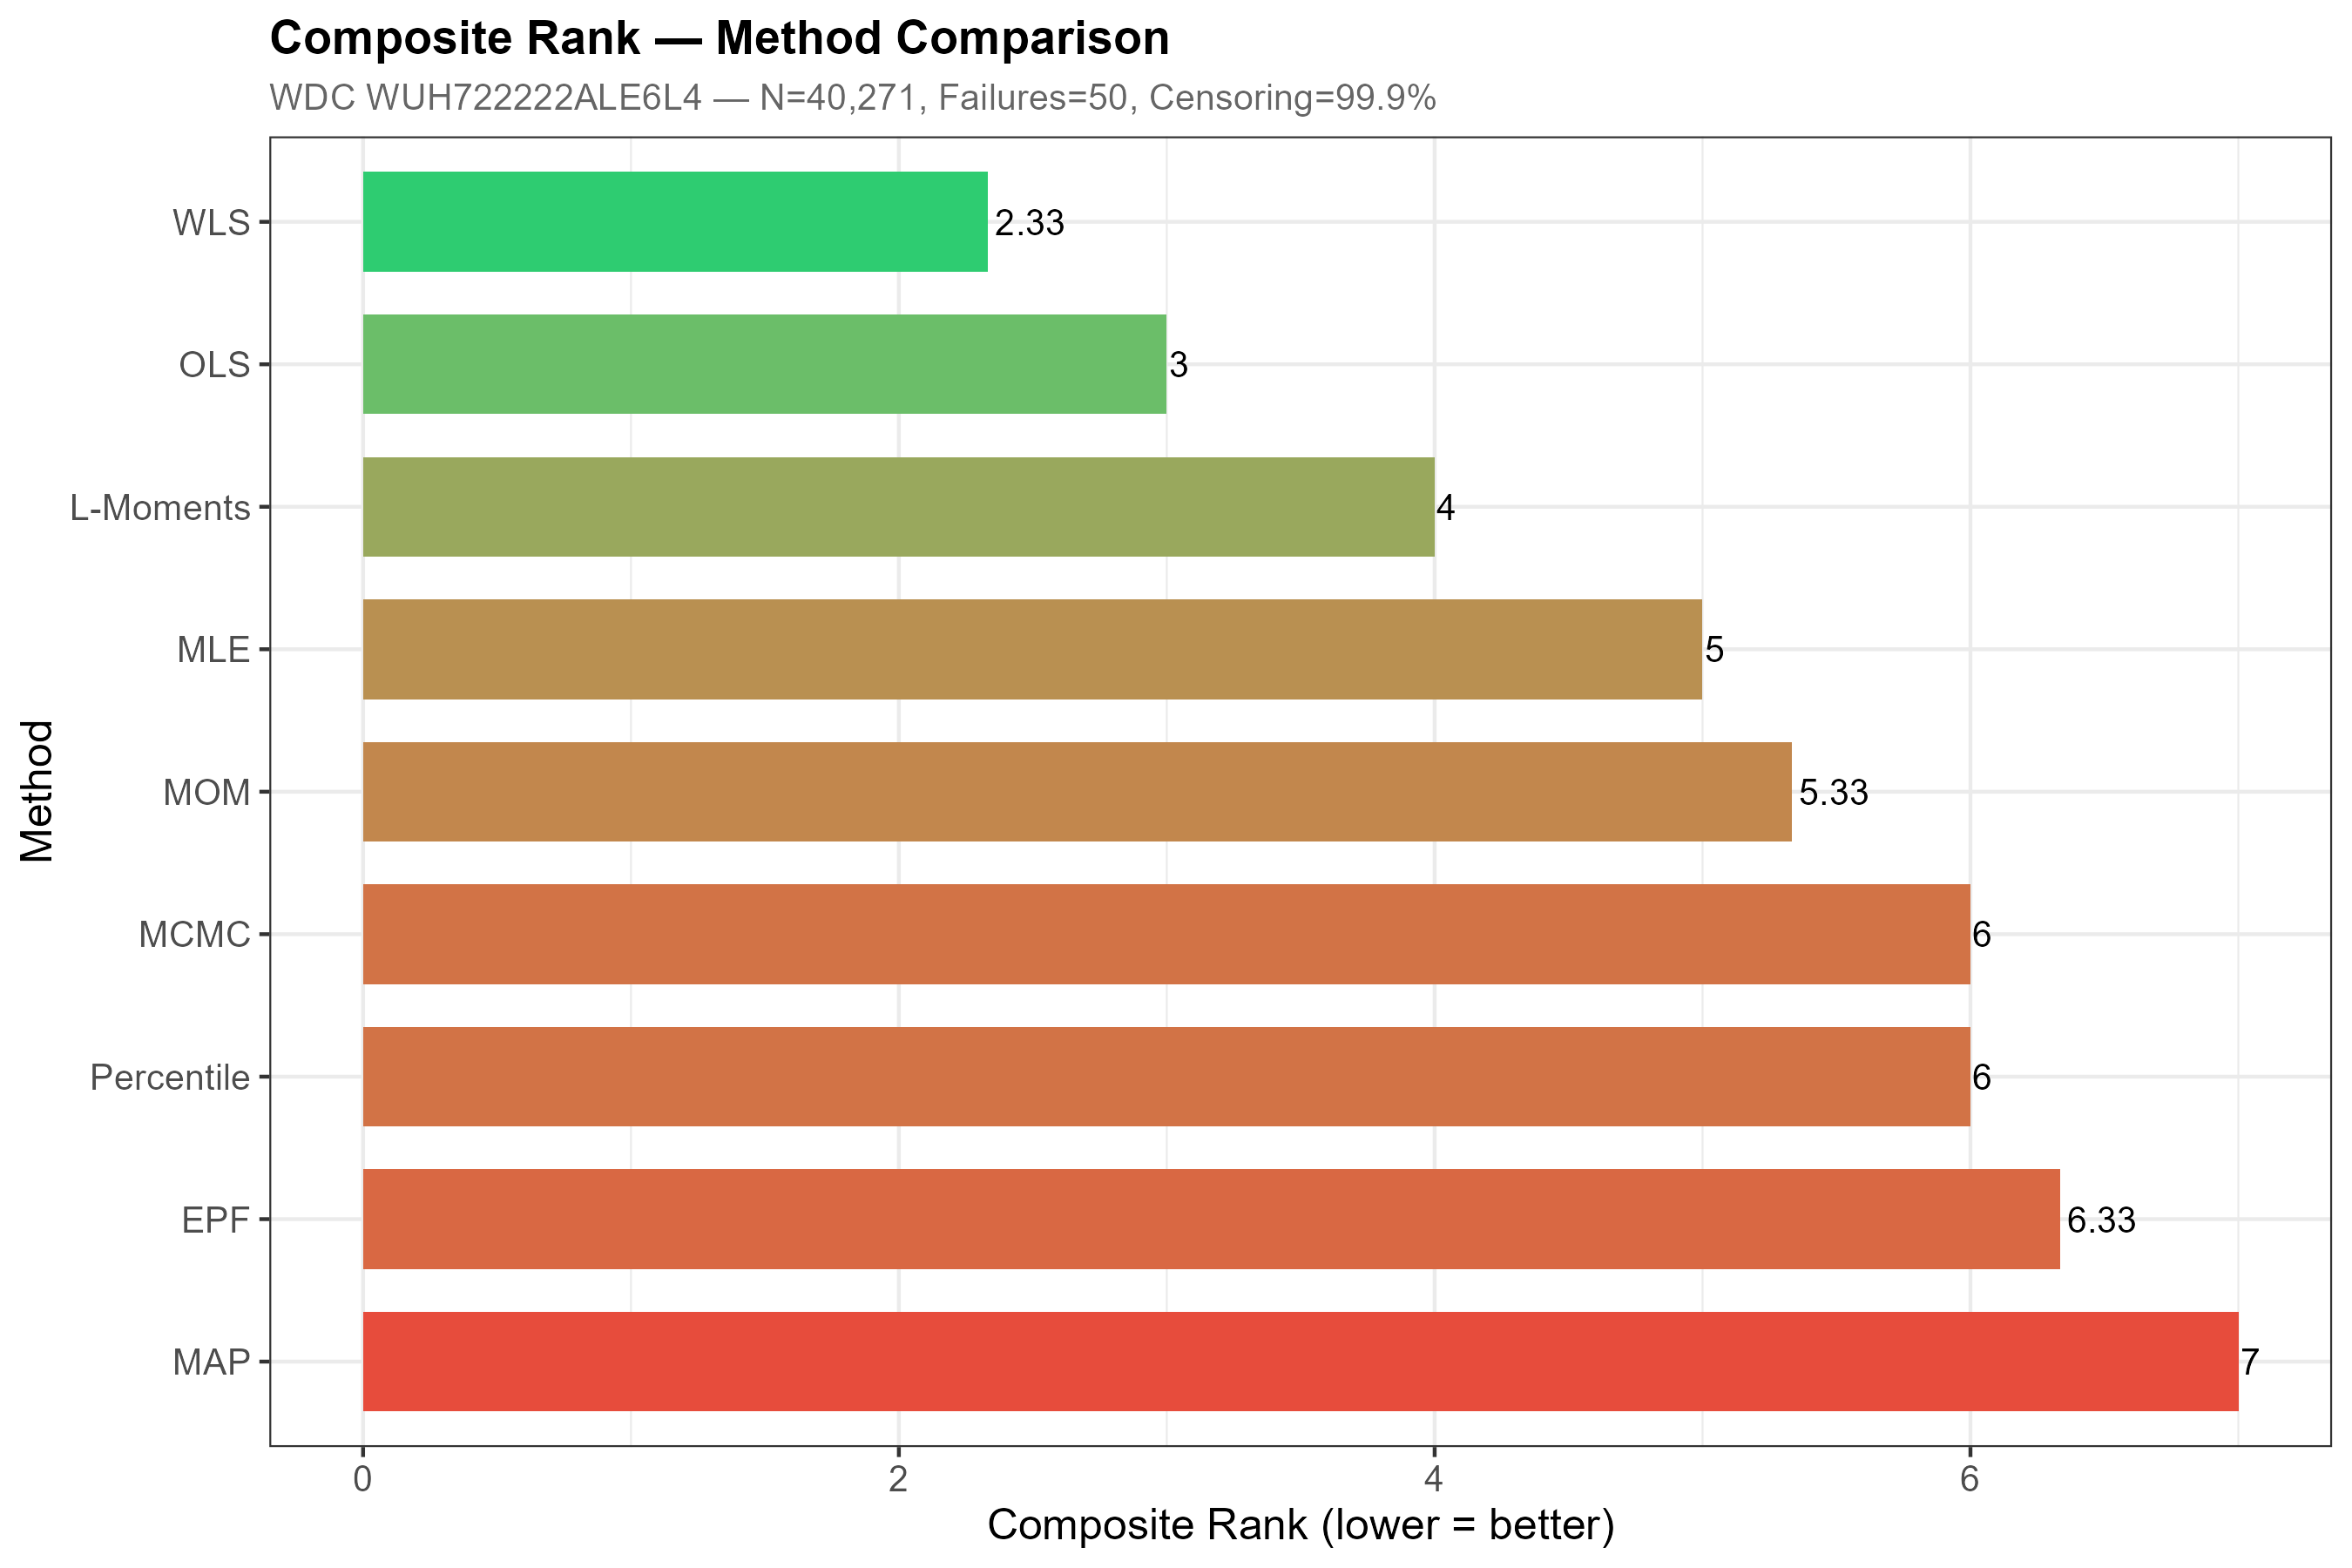
\includegraphics[width=0.95\linewidth]{results/plots/plot7_composite_rank_WDC_WUH722222ALE6L4.png}
\caption{plot7 composite rank — WDC WUH722222ALE6L4}
\end{figure}

\begin{figure}[H]
\centering
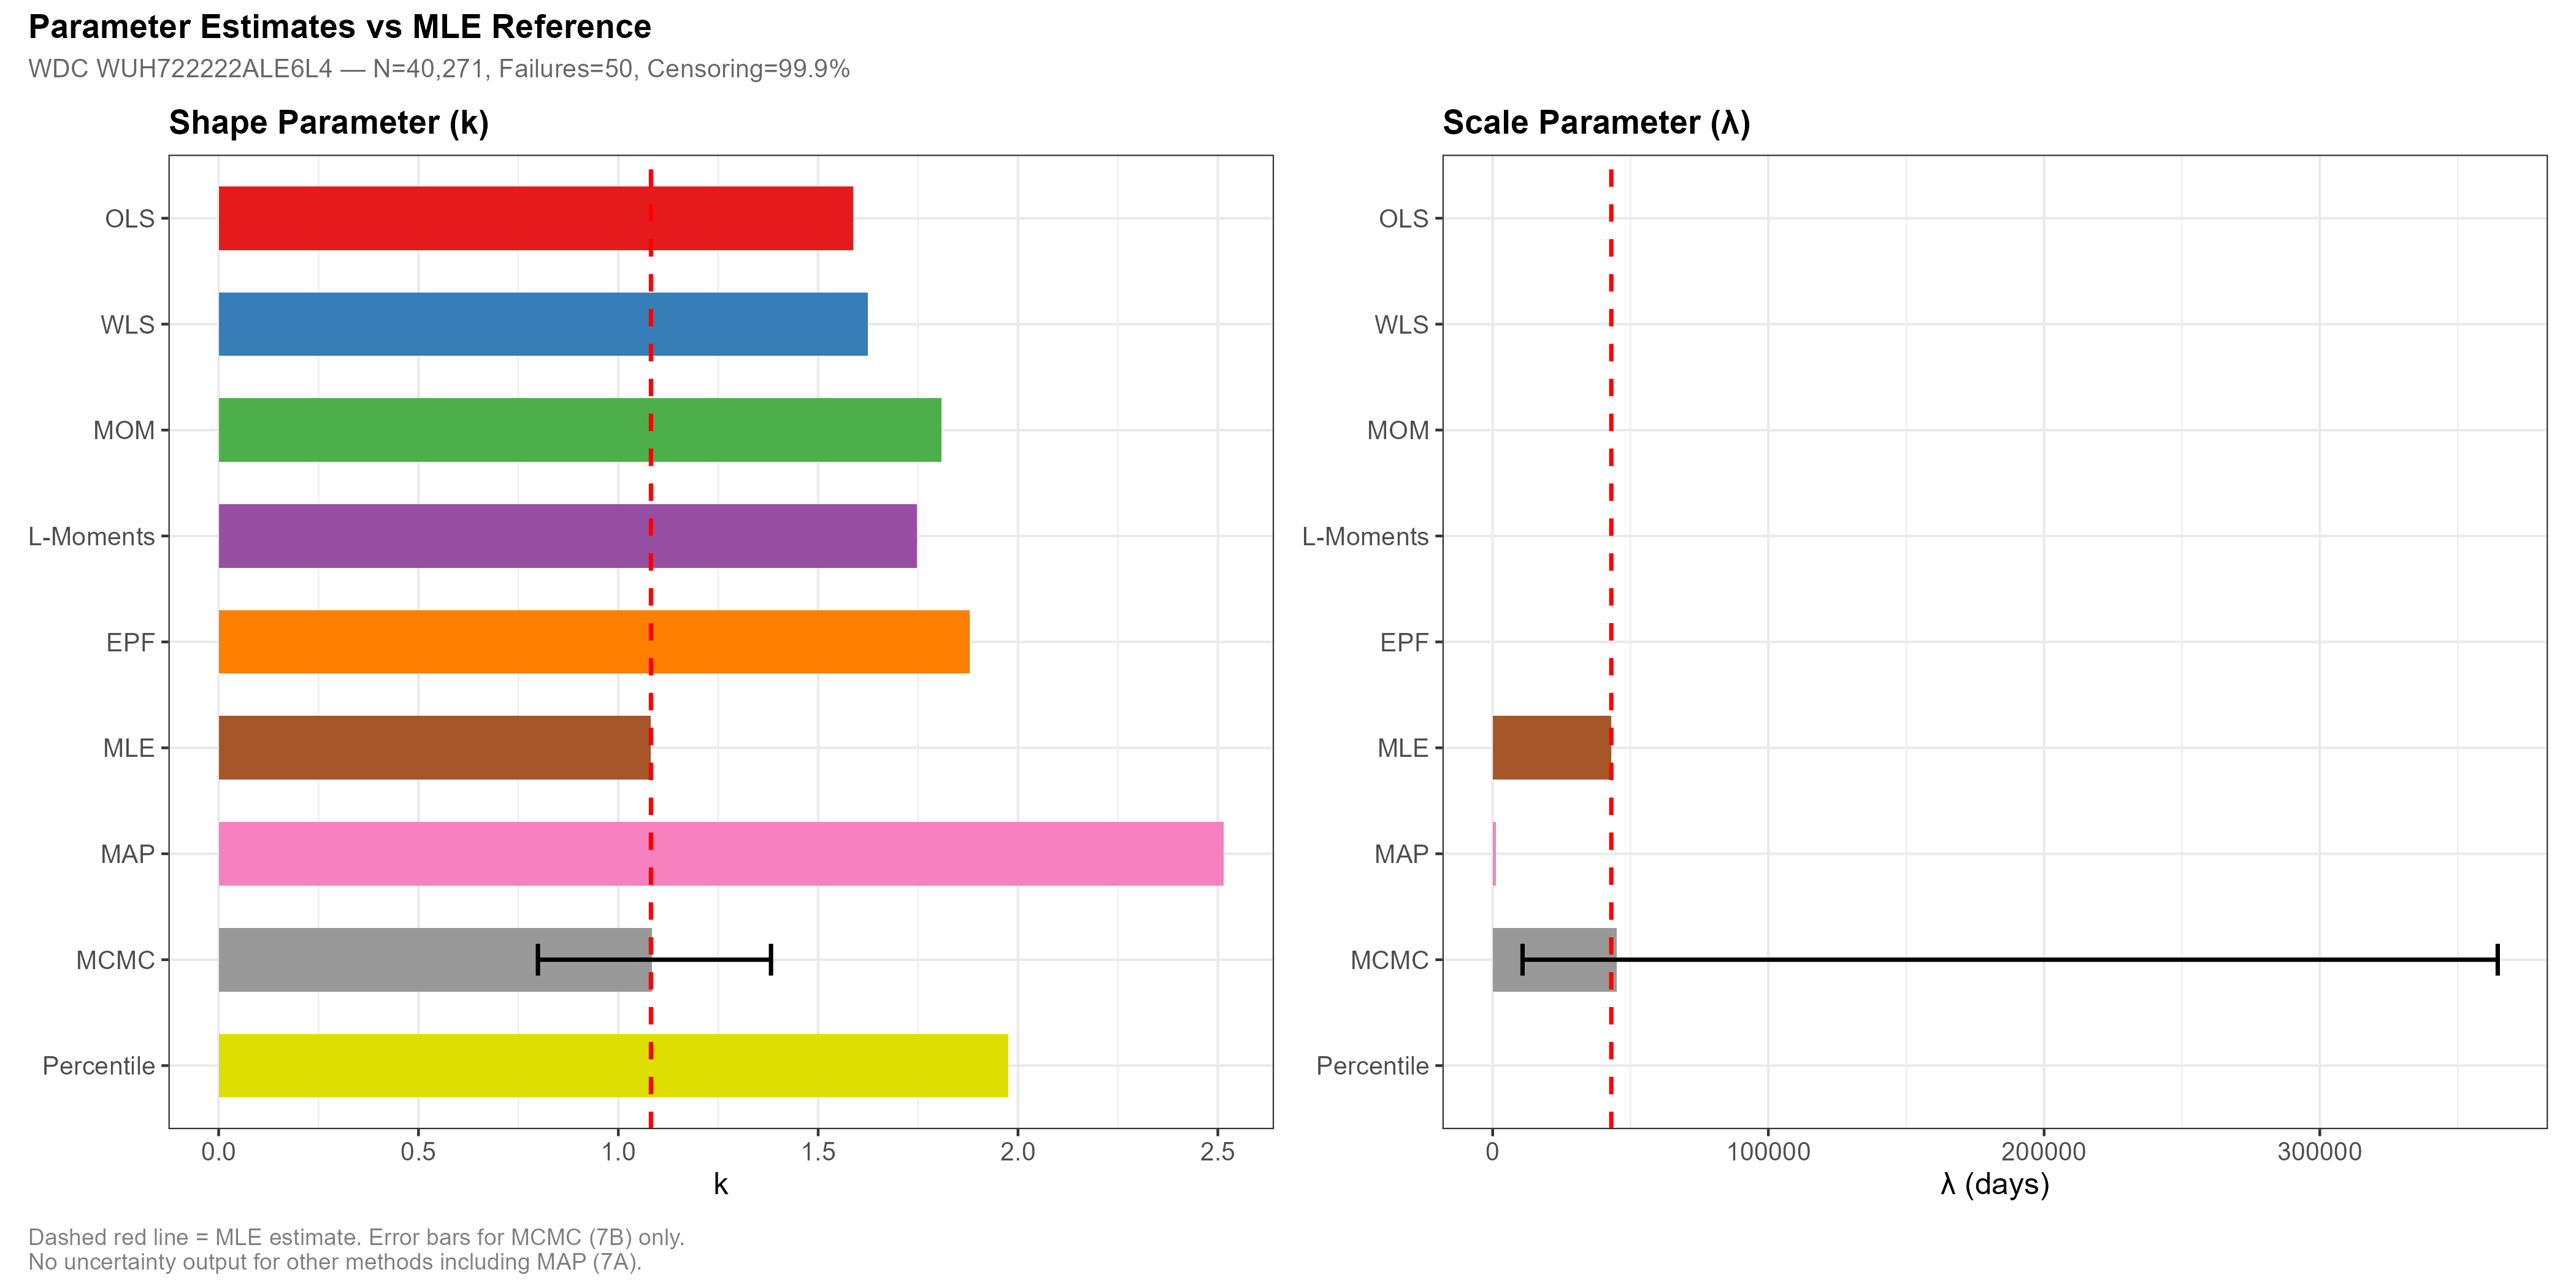
\includegraphics[width=0.95\linewidth]{results/plots/plot8_parameters_WDC_WUH722222ALE6L4.png}
\caption{plot8 parameters — WDC WUH722222ALE6L4}
\end{figure}

\section{Decision Logic}\label{decision-logic}

\begin{Shaded}
\begin{Highlighting}[]
\NormalTok{decision\_df }\OtherTok{\textless{}{-}} \FunctionTok{tibble}\NormalTok{(}
  \StringTok{\textasciigrave{}}\AttributeTok{Censoring Level}\StringTok{\textasciigrave{}} \OtherTok{=} \FunctionTok{c}\NormalTok{(}\StringTok{"\textgreater{} 0\%"}\NormalTok{, }\StringTok{"\textgreater{} 0\%"}\NormalTok{, }\StringTok{"\textgreater{} 0\%"}\NormalTok{, }\StringTok{"\textgreater{} \textasciitilde{}5\%"}\NormalTok{, }\StringTok{"\textgreater{} \textasciitilde{}20\%"}\NormalTok{, }\StringTok{"\textgreater{} \textasciitilde{}20\%"}\NormalTok{,}
                        \StringTok{"Any"}\NormalTok{, }\StringTok{"Any"}\NormalTok{, }\StringTok{"Any"}\NormalTok{),}
  \AttributeTok{Method =} \FunctionTok{c}\NormalTok{(}\StringTok{"Percentile"}\NormalTok{, }\StringTok{"MOM"}\NormalTok{, }\StringTok{"EPF"}\NormalTok{, }\StringTok{"L{-}Moments"}\NormalTok{, }\StringTok{"OLS"}\NormalTok{, }\StringTok{"WLS"}\NormalTok{,}
             \StringTok{"MLE"}\NormalTok{, }\StringTok{"MAP"}\NormalTok{, }\StringTok{"MCMC"}\NormalTok{),}
  \AttributeTok{Action =} \FunctionTok{c}\NormalTok{(}\StringTok{"Eliminate"}\NormalTok{, }\StringTok{"Eliminate"}\NormalTok{, }\StringTok{"Eliminate"}\NormalTok{, }\StringTok{"Eliminate"}\NormalTok{,}
             \StringTok{"Eliminate"}\NormalTok{, }\StringTok{"Eliminate"}\NormalTok{, }\StringTok{"Retain"}\NormalTok{, }\StringTok{"Retain"}\NormalTok{, }\StringTok{"Retain"}\NormalTok{),}
  \AttributeTok{Reason =} \FunctionTok{c}\NormalTok{(}\StringTok{"Cannot place censored units on CDF"}\NormalTok{,}
             \StringTok{"Sample mean biased downward"}\NormalTok{,}
             \StringTok{"Cannot include censored obs in E[v³]"}\NormalTok{,}
             \StringTok{"L{-}stats over failures only — biased \textgreater{}5\%"}\NormalTok{,}
             \StringTok{"Rank{-}based, no censoring mechanism"}\NormalTok{,}
             \StringTok{"Rank{-}based, no censoring mechanism"}\NormalTok{,}
             \StringTok{"Censored loglik handles natively"}\NormalTok{,}
             \StringTok{"Same loglik + prior regularization"}\NormalTok{,}
             \StringTok{"Full posterior with censoring (extension)"}\NormalTok{)}
\NormalTok{)}

\NormalTok{decision\_df }\SpecialCharTok{\%\textgreater{}\%}
  \FunctionTok{kable}\NormalTok{(}\AttributeTok{caption =} \StringTok{"Method Elimination Rules by Censoring Level"}\NormalTok{,}
        \AttributeTok{booktabs =} \ConstantTok{TRUE}\NormalTok{) }\SpecialCharTok{\%\textgreater{}\%}
  \FunctionTok{kable\_styling}\NormalTok{(}\AttributeTok{latex\_options =} \FunctionTok{c}\NormalTok{(}\StringTok{"striped"}\NormalTok{, }\StringTok{"hold\_position"}\NormalTok{))}
\end{Highlighting}
\end{Shaded}

\begin{longtable}[t]{llll}
\caption{\label{tab:decision-table}Method Elimination Rules by Censoring Level}\\
\toprule
Censoring Level & Method & Action & Reason\\
\midrule
\cellcolor{gray!10}{> 0\%} & \cellcolor{gray!10}{Percentile} & \cellcolor{gray!10}{Eliminate} & \cellcolor{gray!10}{Cannot place censored units on CDF}\\
> 0\% & MOM & Eliminate & Sample mean biased downward\\
\cellcolor{gray!10}{> 0\%} & \cellcolor{gray!10}{EPF} & \cellcolor{gray!10}{Eliminate} & \cellcolor{gray!10}{Cannot include censored obs in E[v³]}\\
> \textasciitilde{}5\% & L-Moments & Eliminate & L-stats over failures only — biased >5\%\\
\cellcolor{gray!10}{> \textasciitilde{}20\%} & \cellcolor{gray!10}{OLS} & \cellcolor{gray!10}{Eliminate} & \cellcolor{gray!10}{Rank-based, no censoring mechanism}\\
\addlinespace
> \textasciitilde{}20\% & WLS & Eliminate & Rank-based, no censoring mechanism\\
\cellcolor{gray!10}{Any} & \cellcolor{gray!10}{MLE} & \cellcolor{gray!10}{Retain} & \cellcolor{gray!10}{Censored loglik handles natively}\\
Any & MAP & Retain & Same loglik + prior regularization\\
\cellcolor{gray!10}{Any} & \cellcolor{gray!10}{MCMC} & \cellcolor{gray!10}{Retain} & \cellcolor{gray!10}{Full posterior with censoring (extension)}\\
\bottomrule
\end{longtable}

\section{Conclusion}\label{conclusion}

\begin{Shaded}
\begin{Highlighting}[]
\ControlFlowTok{for}\NormalTok{ (mdl }\ControlFlowTok{in}\NormalTok{ models) \{}
\NormalTok{  model\_gof }\OtherTok{\textless{}{-}}\NormalTok{ gof }\SpecialCharTok{\%\textgreater{}\%} \FunctionTok{filter}\NormalTok{(model }\SpecialCharTok{==}\NormalTok{ mdl, }\SpecialCharTok{!}\FunctionTok{is.na}\NormalTok{(Composite\_Rank))}
\NormalTok{  best }\OtherTok{\textless{}{-}}\NormalTok{ model\_gof }\SpecialCharTok{\%\textgreater{}\%} \FunctionTok{arrange}\NormalTok{(Composite\_Rank) }\SpecialCharTok{\%\textgreater{}\%} \FunctionTok{slice}\NormalTok{(}\DecValTok{1}\NormalTok{)}
  \FunctionTok{cat}\NormalTok{(}\StringTok{"**"}\NormalTok{, mdl, }\StringTok{"**: Best method ="}\NormalTok{, best}\SpecialCharTok{$}\NormalTok{method,}
      \StringTok{"(Composite Rank ="}\NormalTok{, }\FunctionTok{round}\NormalTok{(best}\SpecialCharTok{$}\NormalTok{Composite\_Rank, }\DecValTok{2}\NormalTok{), }\StringTok{")}\SpecialCharTok{\textbackslash{}n\textbackslash{}n}\StringTok{"}\NormalTok{)}
\NormalTok{\}}
\end{Highlighting}
\end{Shaded}

\begin{verbatim}
## ** TOSHIBA MG07ACA14TA **: Best method = WLS (Composite Rank = 2.67 )
## 
## ** TOSHIBA MG08ACA16TA **: Best method = WLS (Composite Rank = 2 )
## 
## ** WDC WUH722222ALE6L4 **: Best method = WLS (Composite Rank = 2.33 )
\end{verbatim}

\section{Sensitivity Analysis}\label{sensitivity-analysis}

\begin{Shaded}
\begin{Highlighting}[]
\NormalTok{sens }\OtherTok{\textless{}{-}} \FunctionTok{read\_csv}\NormalTok{(}\StringTok{"results/sensitivity\_analysis.csv"}\NormalTok{,}
                 \AttributeTok{show\_col\_types =} \ConstantTok{FALSE}\NormalTok{)}
\NormalTok{sens }\SpecialCharTok{\%\textgreater{}\%}
  \FunctionTok{mutate}\NormalTok{(}\FunctionTok{across}\NormalTok{(}\FunctionTok{where}\NormalTok{(is.numeric), }\SpecialCharTok{\textasciitilde{}}\FunctionTok{round}\NormalTok{(., }\DecValTok{3}\NormalTok{))) }\SpecialCharTok{\%\textgreater{}\%}
  \FunctionTok{kable}\NormalTok{(}\AttributeTok{caption =} \StringTok{"EPF Outlier Sensitivity — Largest Failure Time × 10"}\NormalTok{,}
        \AttributeTok{booktabs =} \ConstantTok{TRUE}\NormalTok{) }\SpecialCharTok{\%\textgreater{}\%}
  \FunctionTok{kable\_styling}\NormalTok{(}\AttributeTok{latex\_options =} \FunctionTok{c}\NormalTok{(}\StringTok{"striped"}\NormalTok{, }\StringTok{"hold\_position"}\NormalTok{))}
\end{Highlighting}
\end{Shaded}

\begin{longtable}[t]{lrrrl}
\caption{\label{tab:sensitivity}EPF Outlier Sensitivity — Largest Failure Time × 10}\\
\toprule
method & k\_clean & k\_contaminated & pct\_change & model\\
\midrule
\cellcolor{gray!10}{EPF} & \cellcolor{gray!10}{1.921} & \cellcolor{gray!10}{0.566} & \cellcolor{gray!10}{70.549} & \cellcolor{gray!10}{TOSHIBA MG07ACA14TA}\\
MOM & 1.799 & 0.644 & 64.200 & TOSHIBA MG07ACA14TA\\
\cellcolor{gray!10}{L-Moments} & \cellcolor{gray!10}{1.719} & \cellcolor{gray!10}{1.265} & \cellcolor{gray!10}{26.452} & \cellcolor{gray!10}{TOSHIBA MG07ACA14TA}\\
MLE & 1.646 & 1.055 & 35.914 & TOSHIBA MG07ACA14TA\\
\cellcolor{gray!10}{EPF} & \cellcolor{gray!10}{2.202} & \cellcolor{gray!10}{0.574} & \cellcolor{gray!10}{73.933} & \cellcolor{gray!10}{TOSHIBA MG08ACA16TA}\\
\addlinespace
MOM & 2.083 & 0.639 & 69.317 & TOSHIBA MG08ACA16TA\\
\cellcolor{gray!10}{L-Moments} & \cellcolor{gray!10}{2.013} & \cellcolor{gray!10}{1.329} & \cellcolor{gray!10}{33.986} & \cellcolor{gray!10}{TOSHIBA MG08ACA16TA}\\
MLE & 2.075 & 1.092 & 47.379 & TOSHIBA MG08ACA16TA\\
\cellcolor{gray!10}{EPF} & \cellcolor{gray!10}{1.879} & \cellcolor{gray!10}{0.524} & \cellcolor{gray!10}{72.114} & \cellcolor{gray!10}{WDC WUH722222ALE6L4}\\
MOM & 1.808 & 0.528 & 70.784 & WDC WUH722222ALE6L4\\
\addlinespace
\cellcolor{gray!10}{L-Moments} & \cellcolor{gray!10}{1.747} & \cellcolor{gray!10}{0.971} & \cellcolor{gray!10}{44.413} & \cellcolor{gray!10}{WDC WUH722222ALE6L4}\\
MLE & 1.804 & 0.938 & 48.026 & WDC WUH722222ALE6L4\\
\bottomrule
\end{longtable}

EPF shows the largest \% change in \(k\) under contamination, confirming
theoretical prediction. L-Moments shows the smallest change (linear
combinations). MLE is moderate (log-likelihood dampens extremes).

\newpage

\section{Session Info}\label{session-info}

\begin{Shaded}
\begin{Highlighting}[]
\FunctionTok{sessionInfo}\NormalTok{()}
\end{Highlighting}
\end{Shaded}

\begin{verbatim}
## R version 4.5.2 (2025-10-31 ucrt)
## Platform: x86_64-w64-mingw32/x64
## Running under: Windows 11 x64 (build 26200)
## 
## Matrix products: default
##   LAPACK version 3.12.1
## 
## locale:
## [1] LC_COLLATE=French_Tunisia.utf8  LC_CTYPE=French_Tunisia.utf8   
## [3] LC_MONETARY=French_Tunisia.utf8 LC_NUMERIC=C                   
## [5] LC_TIME=French_Tunisia.utf8    
## 
## time zone: Africa/Tunis
## tzcode source: internal
## 
## attached base packages:
## [1] stats     graphics  grDevices utils     datasets  methods   base     
## 
## other attached packages:
##  [1] kableExtra_1.4.0 knitr_1.51       here_1.0.2       lubridate_1.9.5 
##  [5] forcats_1.0.1    stringr_1.6.0    dplyr_1.2.1      purrr_1.2.2     
##  [9] readr_2.2.0      tidyr_1.3.2      tibble_3.3.1     ggplot2_4.0.2   
## [13] tidyverse_2.0.0 
## 
## loaded via a namespace (and not attached):
##  [1] generics_0.1.4     xml2_1.5.2         stringi_1.8.7      hms_1.1.4         
##  [5] digest_0.6.39      magrittr_2.0.5     evaluate_1.0.5     grid_4.5.2        
##  [9] timechange_0.4.0   RColorBrewer_1.1-3 fastmap_1.2.0      rprojroot_2.1.1   
## [13] viridisLite_0.4.3  scales_1.4.0       textshaping_1.0.5  cli_3.6.6         
## [17] rlang_1.2.0        crayon_1.5.3       bit64_4.6.0-1      withr_3.0.2       
## [21] yaml_2.3.12        parallel_4.5.2     tools_4.5.2        tzdb_0.5.0        
## [25] vctrs_0.7.3        R6_2.6.1           lifecycle_1.0.5    bit_4.6.0         
## [29] vroom_1.7.1        pkgconfig_2.0.3    pillar_1.11.1      gtable_0.3.6      
## [33] glue_1.8.1         systemfonts_1.3.2  xfun_0.57          tidyselect_1.2.1  
## [37] rstudioapi_0.18.0  farver_2.1.2       htmltools_0.5.9    rmarkdown_2.31    
## [41] svglite_2.2.2      compiler_4.5.2     S7_0.2.1
\end{verbatim}

\end{document}
